\documentclass[onecolumn, 12pt]{book}

\usepackage[latin1]{inputenc}   
\usepackage{amsmath}
\usepackage{algorithm}
\usepackage{algorithmic} 
%\usepackage[T1]{fontenc}

%\usepackage[francais]{babel}     
\usepackage{layout}    
\usepackage[top=2cm, bottom=2cm, left=2cm, right=2cm]{geometry} 
\usepackage{setspace}
\usepackage{soul}
\usepackage{color} 
\usepackage{verbatim}
\usepackage{moreverb}
\usepackage{listings}
\usepackage{url}
\usepackage{graphicx}
%\usepackage{epstopdf}
%\usepackage[outdir=/home/willy/Documents/latexDoc/redaction/fusion_fichiers/images_fusionChapitres/]{epstopdf}
%\usepackage[outdir=./../../fusion_fichiers/images_fusionChapitres/]{epstopdf}
\usepackage[outdir=./]{epstopdf}
\usepackage{caption}
\usepackage{setspace}
\usepackage{enumitem} 
\usepackage{amsthm} % ajouter pour environnement proof
\usepackage{placeins}
\usepackage{multirow}

 \newcounter{subsubsubsection}
\renewcommand\thesubsubsubsection{\thesubsubsection.\arabic{subsubsubsection}}
\renewcommand\theparagraph{\thesubsubsubsection.\arabic{paragraph}} % optional; useful if paragraphs are to be numbered
\setcounter{secnumdepth}{4}
\setcounter{tocdepth}{4}

\title{Chapitre6 : Exp\'erimentations sur des donn\'ees al\'eatoires}
\author{Wilfried Ehounou}
\date{\oldstylenums{\today}} 


%--- d\'efinition macro ------
\def\R{\mbox{I\hspace{-.15em}R}}
\def\N{\mbox{I\hspace{-.15em}N}}
\def\Z{\mbox{I\hspace{-.15em}Z}}
\def\Q{\mbox{I\hspace{-.15em}Q}}

\newtheorem{definition}{D\'efinition}
\newtheorem{theorem}{Th\'eor\`eme}
\newtheorem{property}{Propri\'et\'e}
\newtheorem{claim}[theorem]{Claim}
\newtheorem{proposition}[theorem]{Proposition}
\newtheorem{lemma}[theorem]{Lemma}
\newtheorem{corollary}[theorem]{Corollary}
\newtheorem{conjecture}[theorem]{Conjecture}
\newtheorem{observation}{Observation}
\newtheorem{example}{Exemple}
\newtheorem{remark}{Remarque}

%---- path figures ----
\graphicspath{
{/home/willy/Documents/latexDoc/redaction/fusion_fichiers/images_fusionChapitres/}
}
 
\begin{document}
\maketitle
\tableofcontents

\chapter{\'Evaluation des performances des algorithmes}
\label{chapitreEvaluation}

Dans ce chapitre, nous g\'en\'erons des topologies de r\'eseaux \'electriques qui sont des DAG sans circuits. \`A partir de ces topologies, nous construisons leurs line-graphes  que nous modifions selon  deux approches.
%nous disposons des line-graphes que nous modifions de deux mani\`eres. 
La premi\`ere approche consiste \`a changer les valeurs de $k$ cases choisies al\'eatoirement.
La seconde approche construit une matrice associ\'ee au line-graphe du DAG dont chaque case contient une valeur de probabilit\'e puis applique une valeur de seuil sur cette matrice pour en d\'eduire une matrice d'adjacence. De ce fait, cette matrice d'adjacence contient des cases modifi\'ees qui seront d\'esign\'ees par {\em erreurs}. 
\newline
Notre objectif est d'\'evaluer les performances de notre couple d'algorithmes sur ces line-graphes modifi\'es c'est-\`a-dire la capacit\'e de nos algorithmes \`a corriger les {\em erreurs}.
 Pour ce faire, nous divisons ce chapitre en quatre parties. 
 La premi\`ere partie d\'ecrit la g\'en\'eration de graphes \'electriques (les DAG) et la construction de leurs line-graphes associ\'es. 
 Ensuite, la seconde partie pr\'esente les diff\'erentes \'etapes de la modification des $k$ cases des line-graphes, le protocole d'exp\'erimentation et l'analyse des r\'esultats.
 La troisi\`eme partie  analyse les performances des algorithmes sur des
 line-graphes modifi\'es par la deuxi\`eme approche.
 Enfin, dans la derni\`ere partie, nous analysons ces performances sur des graphes dit {\em grilles boucl\'ees}. Dans ces graphes, chaque sommet n'est couvert par aucune clique.

\section{G\'en\'eration de graphes \'electriques}
	\label{generationGraphesElectriques}
	La topologie du r\'eseau \'electrique est repr\'esent\'ee par un graphe orient\'e sans circuit $G$.
Les c\^ables \'electriques sont unidirectionnels et les \'equipements sont toujours aliment\'es par une source. Ce qui implique que le courant se propage dans une direction et cette direction  indique l'orientation des arcs d'un {\em DAG} ({\em Directed Acyclic Graph}).
Nous allons d\'ecrire comment nous g\'en\'erons le graphe $G$.
\newline
Consid\'erons un graphe non orient\'e $G=(V, E)$ dans lequel  $V$ est l'ensemble de $n$ sommets, $E$ l'ensemble des $m$ ar\^etes et $\alpha$ son degr\'e moyen choisi. 
La probabilit\'e d'existence d'une ar\^ete entre deux sommets est de $\frac{\alpha}{n}$. 
Afin de g\'en\'erer un tel graphe apr\`es avoir choisi $n$ et $\alpha$, nous s\'electionnons  deux sommets $x$ et $y$ de $V$ et nous g\'en\'erons une valeur $p_{xy}$ qui suit  une loi de probabilit\'e uniforme.
Si $p_{xy}$ est sup\'erieure \`a la probabilit\'e d'existence d'une ar\^ete alors nous ajoutons l'ar\^ete $[x,y]$ \`a $E$.
\newline
Si $G$ n'est pas connexe, nous choisissons al\'eatoirement un sommet dans chaque composante connexe et nous ajoutons une ar\^ete entre ces sommets.  Nous obtenons alors  $m$ ar\^etes.
\newline
Afin d'orienter $G$ comme un $DAG$, nous s\'electionnons de fa\c con al\'eatoire quatre sommets  de degr\'e minimum pour les d\'efinir comme les sources de notre tri topologique.
Nous effectuons ce tri avec un parcours en largeur {\em Breast First Search (BFS)} dans le graphe $G$. 
Chaque sommet $x$ obtient un ordre topologique $D_x$ et l'ar\^ete $e_{xy}$ devient 
soit l'arc $a_{xy}$ si $D_x < D_y$ 
soit l'arc $a_{yx}$ si $D_x > D_y$. 
Les arcs $a_{xy}$ forment l'ensemble $A$ des arcs de $G$. 
Nous en d\'eduisons que $G=(V, A)$ est orient\'e et son line-graphe $LG$ est construit \`a partir de la d\'efinition \ref{definitionLineGraphe}.
\newline
Nous notons $M_{G}$  la matrice d'adjacence de $G$ et $M_{LG}$ la matrice d'adjacence du line-graphe $LG$.


%-----------------------------------------------------------------------
%------- 		experimentation 1     ---------------------
%--------------------------------------------------------------------
\section{Exp\'erimentation 1 : modification de $k$ cases  de la matrice du line-graphe}
	\label{experimentation1}
	\subsection{S\'election de $k$ cases et g\'en\'eration de la matrice $M_{k,p}$ }
		Nous modifions $k$ cases de la matrice d'adjacence $M_{LG}$. Ces cases sont choisies de mani\`ere al\'eatoire. Afin de contr\^oler la proportion des cases \`a modifier dont la valeur initiale est $0$ ou $1$,  nous introduisons la probabilit\'e $p$.
\newline
Soit donc $p  \in [0,1]$ la variable qui d\'esigne la proportion de cases \`a $0$ s\'electionn\'ees. La proportion de cases \`a $1$ est donc $1-p$.
Par exemple, $p = 0.5$ signifie que $50\%$ des cases s\'electionn\'ees sont des cases \`a $0$ et $50\%$ des autres cases s\'electionn\'ees sont des cases \`a $1$. 
De m\^eme, les $k$ cases sont des cases \`a $1$ si $p = 0$ et elles sont des cases \`a $0$ si $p = 1$. 
 Avec la repartition $p$, nous calculons les nombres $n_0$ de cases \`a $0$ et $n_1$ de cases \`a $1$. Ces cases sont \`a modifier dans $M_{LG}$. 
Ensuite nous s\'electionnons uniformement $n_0$ cases \`a $0$ et $n_1$ cases \`a $1$ dans la matrice $M_{LG}$.
Les cases \`a $0$ sont chang\'ees en $1$ et les cases \`a $1$ sont chang\'ees en $0$.
La nouvelle matrice d'adjacence $M_{k,p}$ contient quatre types de cases :
\begin{itemize}
	\item Si $M_{k,p} [i,j] = M_{LG} [i,j] = 0$ alors $M_{k,p} [i,j]$ est dit {\em vrai n\'egatif}. 
	\item Si $M_{k,p} [i,j] = M_{LG} [i,j] = 1$ alors $M_{k,p} [i,j]$ est dit {\em vrai positif}. 
	\item Si $M_{k,p} [i,j] = 0$ et $M_{LG} [i,j] = 1$ alors $M_{k,p} [i,j]$ est dit {\em faux n\'egatif}.
	\item Si $M_{k,p} [i,j] = 1$ et $M_{LG} [i,j] = 0$ alors $M_{k,p} [i,j]$ est dit {\em faux positif}.
\end{itemize}
La matrice $M_{k,p}$ est la matrice d'adjacence du graphe $G_{k,p}$ et ce graphe a le m\^eme ensemble de sommets que $LG$ mais leur ensemble d'ar\^etes diff\`ere de $k$ ar\^etes.
G\'en\'eralement, $G_{k,p}$ n'est pas un line-graphe. Toutefois, s'il est un line-graphe alors il est  impossible que $G_{k,p}$ soit le line-graphe de $G$. 
	\subsection{Protocole d'exp\'erimentation sur les graphes $G_{k,p}$}
		L'application de nos algorithmes de d\'ecouverte et de correction d\'ebute par la g\'en\'eration de $500$ topologies \'electriques $G$ de $30$ sommets, chacune ayant un degr\'e maximal moyen de  $\Delta(G) = 5$.
Nous construisons $500$ line-graphes $LG$ de $150$ sommets et $470$ ar\^etes, en moyenne. \newline
Nous avons donc introduit trois param\`etres $k, p,  \alpha_{max}$:
\begin{enumerate}
\item Le param\`etre $k$ d\'esigne le nombre de cases modifi\'ees dans la matrice $M_{LG}$. Dans notre \'etude, $k \in \{1,\cdots,9\}$.
\item Le param\`etre $p$ d\'esigne la proportion de cases \`a $0$ s\'electionn\'ees parmi les $k$ cases. Dans notre \'etude, $p \in \{0.1,\cdots,0.9\}$.
\item Le param\`etre $\alpha_{max}$ d\'esigne le nombre de graphes g\'en\'er\'es pour un couple  $(k, p)$ de valeurs donn\'ees.
%\item Le param\`etre $\alpha = \{1,\cdots, \alpha_{max} \}$ d\'esigne le nombre de fois qu'on modifie $k$ cases dans la  matrice $M_{LG}$ pour une valeur de $p$ donn\'ee. Il est utilis\'e pour faire varier les $k$ cases choisies dans un graphe. 
\end{enumerate}
 
Nous  choisissons $\alpha_{max} = 5$ pour des temps de calculs r\'ealistes. 
Chaque graphe g\'en\'er\'e est identifi\'e par une valeur de  $\alpha \in \{1,\cdots, \alpha_{max} \}$, est not\'e $G_{k,p,\alpha}$ et sa matrice d'adjacence est  $M_{k,p,\alpha}$. 
La valeur $\alpha$ d\'esigne l'indice de modification de $k$ cases dans la  matrice $M_{LG}$ pour une valeur de $p$ donn\'ee. Elle est utilis\'ee pour faire varier les $k$ cases choisies dans un graphe. 
Nous appliquons notre couple d'algorithmes sur une matrice $M_{k,p,\alpha}$ et nous obtenons la matrice $M'_{k,p,\alpha}$ qui est la matrice d'adjacence du line-graphe $LG_{k, p, \alpha}$. 

% a ajouter des distance line et hamming
Pour comparer les ar\^etes entre les graphes $LG_{k,p, \alpha}$ et $G_{k,p, \alpha}$, nous calculons la distance de correction (section \ref{algorithmeCorrection}) not\'ee $DC_{k,p, \alpha}$.
De m\^eme, le nombre d'ar\^etes diff\'erentes entre les graphes $LG_{k,p, \alpha}$ et $LG$ d\'efinit la distance de Hamming $DH_{k,p, \alpha}$.
Nous d\'efinissons par les variables $moy\_DH_{k,p}$ et $moy\_DC_{k,p}$, les moyennes respectives des distances de Hamming (not\'ee $DH_{k,p,\alpha}$) et des distances de correction (not\'ee $DC_{k,p,\alpha}$) pour une valeur donn\'ee de $k$ et pour tout $\alpha \in \{1, \cdots, \alpha_{max}\}$.
\begin{equation}
moy\_DH_{k, p} = \sum_{\alpha = 1}^{ \alpha_{max} } DH_{k, p, \alpha} \hspace{1 em}; 
moy\_DC_{k, p} = \sum_{\alpha = 1}^{ \alpha_{max} } DC_{k, p, \alpha}
\end{equation}

Les diff\'erentes \'etapes de l'exp\'erimentation sont r\'esum\'ees dans la figure \ref{recapProtocoleEtude}. Les \'etapes sont repr\'esent\'ees par des graphes et les phases de modification de ces graphes sont d\'esign\'ees par les fl\`eches unidirectionnelles. Quant aux fl\`eches bidirectionnelles (en rouge), elles indiquent le calcul de distances (de Hamming et de correction). 
% ------------  figure recap Protocole Etude  ----------------------
\begin{figure}[htb!] 
\centering
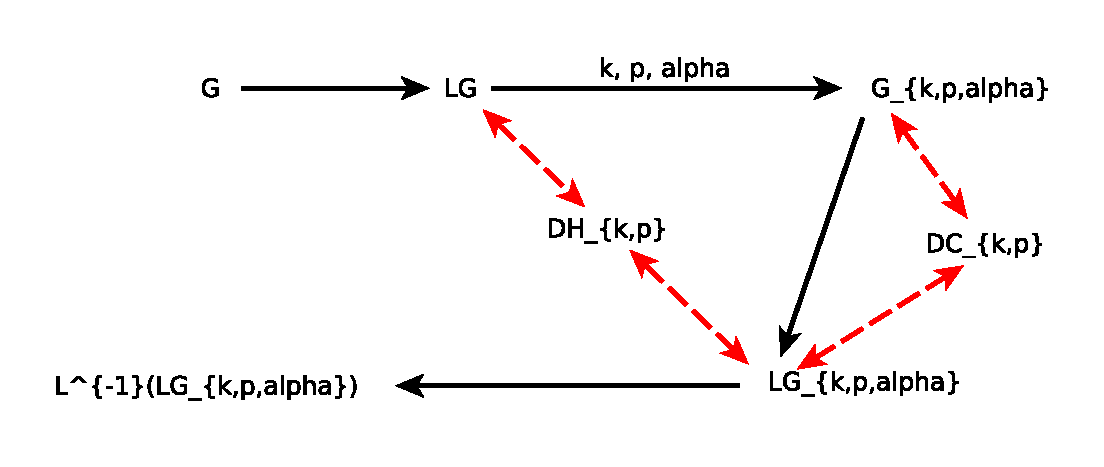
\includegraphics[scale=0.750]{recapProtocoleEtude.eps}
\caption{\'Etapes de l'exp\'erimentation :  \\
1) On g\'en\`ere le graphe $G$ et son line-graphe $LG$;\\ 
2) On modifie $k$ cases la $\alpha^{ieme}$ fois selon la repartition $p$ pour obtenir le graphe $G_{k,p,\alpha}$;\\ 
3) On applique les algorithmes de couverture et de correction pour avoir un line-graphe $LG_{k,p,\alpha}$. $LG_{k,p,\alpha}$ et  $G_{k,p,\alpha}$ diff\`erent de $DC_{k,p,\alpha}$ ar\^etes. $LG_{k,p,\alpha}$ a $DH_{k,p,\alpha}$ cases modifi\'ees par rapport \`a $LG$; 
\\ 4) $L^{-1}(LG_{k,p,\alpha})$ est le graphe racine de $LG_{k,p,\alpha}$. }
\label{recapProtocoleEtude} 
\end{figure}
% ------------  figure recap Protocole Etude  ----------------------
%\FloatBarrier
\newline


% correction du graphe
% 1) comment je selectionne (choisis) les sommets -1
%		- remise: on selectionne un sommet de sommets -1 selon une methode puis on la corrige. Ensuite, on applique notre couple d'algorithme  sur le graphe corrig\'e. On reprend l'operation tant que graphe corrige n'est pas un line-graphe    
%		- sans remise: On choisit une permutation des sommets de sommets-1 puis on les corrige les uns a la suite des autres.Les sommets dans la permutation sont ordonnee selon  la methode suivante:
% 		* degre min : les sommets sont ranges par ordre croissant de leur degre.
%		* cout min : les sommets sont ranges par ordre croissant de leur cout. Le cout est la somme du poids de chaque case modifi\'e.
%		* aleatoire :  les sommets sont ranges sans condition prealable.
%			* aleatoire * cout min * degre min
%correction
Soit ${\cal C}$ l'ensemble des sommets n'\'etant couverts par aucune clique apr\`es l'algorithme de couverture.
La correction de la matrice $M_{k,p,\alpha}$ est n\'ecessaire s'il existe des sommets appartenant \`a ${\cal C}$. 
\newline
Nous distinguons deux modes d'ex\'ecution de notre algorithme de correction:
\begin{enumerate}
	\item Mode avec remise :
				\newline
				\noindent 1. Ex\'ecution algorithme de couverture, {\bf return} ${\cal C}$ \\
				~2. \indent {\bf Tant que} ${\cal C}$ n'est pas vide\\ 
				~3.	       	\indent~~~~~~~~Correction d'un sommet de ${\cal C}$  \\
				~4.	       	\indent~~~~~~~~Ex\'ecution algorithme de couverture, {\bf return} ${\cal C}$ \\
	\item Mode sans remise :
				\newline
				\noindent 1. Ex\'ecution algorithme de couverture, {\bf return} ${\cal C}$ \\
				~2. \indent {\bf Tant que} ${\cal C}$ n'est pas vide\\ 
				~3.	       	\indent~~~~~~~~Correction d'un sommet de ${\cal C}$  \\
				~4.	       	\indent~~~~~~~~Mise \`a jour du sommet  de ${\cal C}$  \\
\end{enumerate}
\`A chaque \'etape $3$ dans les deux modes, un sommet de $\cal C$ est choisi selon :
\begin{enumerate} [label = (\alph*)]
\item {\em Degr\'e minimum} : le sommet de degr\'e minimum est s\'electionn\'e. 
\item {\em Co\^ut minimum} : le sommet de  co\^ut de compression minimum est s\'electionn\'e. Le co\^ut de compression est la somme des co\^uts de chaque case modifi\'ee. 
\item {\em Al\'eatoire} : le sommet est s\'electionn\'e al\'eatoirement parmi les sommets de $\cal C$.
\end{enumerate}
La correction de chaque sommet de ${\cal C}$ implique l'ajout et la suppression des ar\^etes du graphe. Nous souhaitons orienter les d\'ecisions de l'algorithme de correction de telle sorte qu'il ajoute  ou supprime uniquement des ar\^etes ou 
qu'il r\'ealise les deux op\'erations.
 Nous  priorisons une op\'eration en attribuant des co\^uts diff\'erents \`a  la modification d'ar\^etes.
Nous distinguons trois types d'op\'erations que nous appelons {\em fonctions de co\^ut} :
\begin{enumerate}[label=(\roman*)]
\item {\em Unitaire} : l'ajout et la suppression d'une ar\^ete ont un m\^eme co\^ut c'est-\`a-dire $1$.
\item {\em Ajout} : l'ajout d'une ar\^ete a un co\^ut de $1$ et la suppression a un co\^ut de $2$.
\item {\em Suppression} : l'ajout d'une ar\^ete a un co\^ut de $2$ et la suppression a un co\^ut de $1$.
\end{enumerate}
Nous rappelons que la distance de correction n'est pas la somme de toutes les  modifications d'ar\^etes r\'ealis\'ees. En effet, une ar\^ete  supprim\'ee et ajout\'ee plusieurs fois (pour diff\'erents sommets de ${\cal C}$) n'est comptabilis\'ee qu'une fois et son co\^ut est appliqu\'e selon la fonction de co\^ut.
\newline


\'Etant donn\'ee que nous avons $3$ fonctions de co\^ut, $2$ modes de correction et $3$  s\'elections possibles des sommets, nous nous retrouvons avec $18$ approches de correction de sommets et il est fastidieux de les interpr\'eter sur une m\^eme figure.
Ainsi nous nous limitons \`a la fonction de co\^ut {\em unitaire} dans un premier temps et nous consid\'erons les approches de correction suivantes : $1a$, $1b$, $2a$, $2b$, $2c$.  
La lecture de l'approche de correction $(1a)$ est le suivant : $1)$ avec remise et $a)$ le degr\'e minimum.
L'approche $(1c)$ n'est d'aucune utilit\'e car l'algorithme de correction ne parvient pas \`a fournir un line-graphe. En effet, l'ensemble $\cal C$ croit lin\'eairement \`a chaque \'etape de correction et la correction devient une boucle infinie.
Le tableau \ref{tab:recapApprocheCorrection} r\'esume les approches de correction retenues dans l'analyse des performances de l'algorithme de correction.
% ------------ tableau recapitulatif -----------------------
\begin{table}[h]
   \centering
   \caption{\label{tab:recapApprocheCorrection} Tableau r\'ecapitulatif des approches de corrections }
   \begin{tabular}{|l|c|c|r|}
   	\hline
  	Mode & choix sommets & fonction de co\^ut  \\
  	\hline
%  	Sans Remise & Degre Min & unitaire & 1  \\
%  	\cline{1-9}     & \cline{1-3} & ajout       & 1  \\
	 & 
								\multirow{3}{*}{degr\'e minimum} & unitaire \\
															  & & ajout \\
									
												& & suppression \\
											
								\cline{2-3}
	Sans remise						& 
								\multirow{3}{*}{co\^ut minimum} & unitaire \\
															  & & ajout \\
															  & & suppression \\
															  \cline{2-3}								  
							& 
								\multirow{3}{*}{al\'eatoire} & unitaire \\
															  & & ajout \\
															  & & suppression \\
															  \hline
															  \hline									 
	 & 
								\multirow{3}{*}{degr\'e minimum} & unitaire \\
															  & & ajout \\
															  & & suppression \\
															 \cline{2-3}
	Avec remise						& 
								\multirow{3}{*}{co\^ut minimum} & unitaire \\
															  & & ajout \\
															  & & suppression \\
															  \hline															  
   \end{tabular}
\end{table}
% ------------ tableau recapitulatif -----------------------
\newline

Nous recherchons l'approche qui traite le probl\`eme {\em Proxi-Line} c'est-\`a-dire le mode qui majore la distance line de $G_{k,p}$ par la distance de correction entre $LG_{k,p}$ et $G_{k,p}$.
Une fois le meilleur mode trouv\'e, nous comparons les fonctions de co\^ut $i$, $2i$ et $3i$ avec ce mode pour trouver l'influence de la fonction de co\^ut sur les distances de correction.

%---- decription protocole d'etude --> fin
	\subsection{Analyses des r\'esultats }
%	Nous d\'ebutons par l'interpr\'etation des distributions des distances line et de Hamming pour une m\'ethode de correction et une valeur de $p\_correl$ sp\'ecifiques.
%	Ensuite, nous expliquons le choix de la m\'ethode al\'eatoire pour la correction des sommets et nous montrons qu'avec cette m\'ethode, notre couple d'algorithmes resout le probl\`eme {\em proxi-line} pour $k \le 5$ ar\^etes peu importe l'ordre du line-graphe $LG$.
%	Nous pr\'esentons \'egalement le meilleur compromis de la repartition des $k$ cases modifi\'ees et la relation existante entre les distances line et de Hamming.
%	Enfin, nous montrons que la r\'esolution du probl\`eme proxi-line n'a aucun impact sur nos distributions quelques soient la repartition et la priorit\'e  choisies.
	
	Nous d\'ebutons l'interpr\'etation de nos r\'esultats par l'analyse des distributions des distances de Hamming avec l'approche de correction {\em al\'eatoire sans remise} $(2c)$ et  la fonction de co\^ut {\em unitaire} $(3i)$.
	Ensuite, nous expliquons le choix de l'approche $(2c)$  pour la correction des sommets. 
	Nous pr\'esentons \'egalement le meilleur compromis dans la repartition des $k$ cases modifi\'ees et la relation existante entre les distances de correction et de Hamming.
	Enfin,  nous montrons que l'approche $(2c)$ fournit des distributions de distances de correction et de Hamming identiques, quelles que soient la fonction de co\^ut $(i), (2i), (3i)$ et la repartition $k$ choisies.
		\subsubsection{Interpr\'etation du mode de correction {\em al\'eatoire sans remise}}
			\label{experimentation1InterpretationModeAleatoireSansRemise}
			

% debut explication aprroche aleatoire sans remise avec cout unitaire 
Nous supposons que $p=0.5$ c'est-\`a-dire qu'il y'a autant de cases {\em fausses n\'egatives} que de cases {\em fausses positives} dans la matrice $M_{k,p}$.
\newline
Nous repr\'esentons les distributions des distances de correction et de Hamming, la fonction de repartition de la corr\'elation entre ces distances  et la fonction cumulative de la distance de Hamming. 
La distribution des distances de correction indique la proportion de graphes $LG_{k,p,\alpha}$ qui ont le m\^eme ensemble d'ar\^etes que les graphes $G_{k,p,\alpha}$. En ce qui concerne la distribution des distances de Hamming, elle indique  la proportion de graphes $LG_{k,p,\alpha}$ qui ont le m\^eme ensemble d'ar\^etes que les graphes $LG$.
La corr\'elation entre les distances de correction et de Hamming, not\'ee {\em correlation\_DC\_DH}, est calcul\'ee avec la formule \ref{correlation_correction_hamming}. Sa fonction de repartition $F_k(x)$ indique le nombre de corr\'elations inf\'erieures \`a une valeur de corr\'elation $x$ donn\'ee.
Quant \`a la fonction cumulative de la distance de Hamming, elle montre l'\'evolution du nombre de cases modifi\'ees de la matrice $M'_{k,p}$ en fonction du nombre de line-graphes  construits $LG$.
\newline
%\vspace{-0.5cm}
% -------------------- figure simulation_distanceMoyenDLDH_k_0_aleatoire_p_05 ------------------------
\begin{figure}[htb!] 
\centering
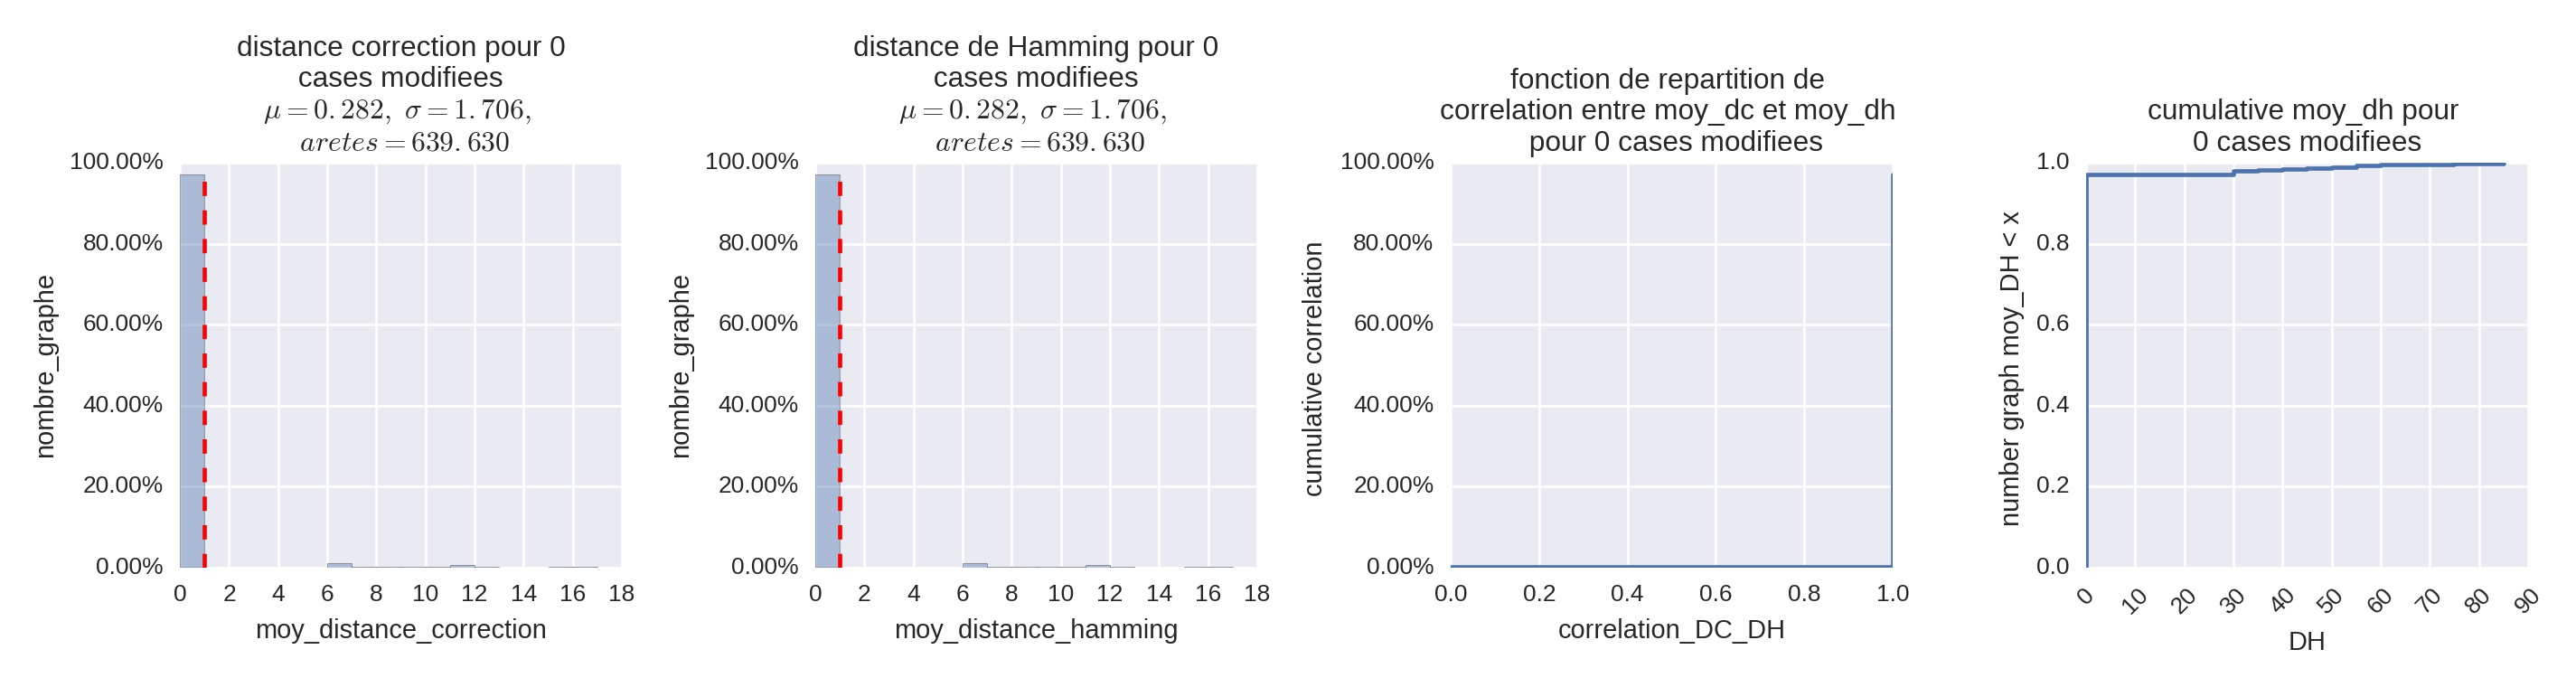
\includegraphics[width=500pt,height=160pt]{simulation_distanceMoyenDLDH_k_0_aleatoire_p_05.jpeg}
\caption{ Approche de correction al\'eatoire sans remise \`a co\^ut unitaire pour $k =0 $ case modifi\'ee. La premi\`ere colonne repr\'esente la distribution des distances de correction $moy\_DC_{0,0.5}$. La seconde colonne est la distribution des distances de Hamming $moy\_DH_{0,0.5}$. La troisi\`eme colonne  est la fonction de repartition de la corr\'elation entre les distances de correction et de Hamming avec en abscisse la corr\'elation entre ces distances (correlation\_DC\_DH).  La quatri\`eme colonne est la fonction cumulative des distances de Hamming.}
\label{sansremise_unitaire_distanceMoyenDCDH_k_0_aleatoire_p_05} 
\end{figure}
\FloatBarrier
% -------------------- figure simulation_distanceMoyenDLDH_k_0_aleatoire_p_05 -----------------------

Les figures \ref{sansremise_unitaire_distanceMoyenDCDH_k_0_aleatoire_p_05} et \ref{sansremise_unitaire_distanceMoyenDCDH_k_1_2_5_9_aleatoire_p_05} pr\'esentent les courbes respectives pour $k=0$ et $k \in \{1,2,5,9\}$ cases modifi\'ees. 
La colonne $1$ indique la distribution des distances de correction, la colonne $2$ est la colonne de la distribution des distances de Hamming, la colonne $3$ est associ\'ee \`a la fonction de repartition de la corr\'elation entre les distances de correction et de Hamming avec en abscisse la corr\'elation entre ces distances ({\em correlation\_DC\_DH)}. 
Et la colonne $4$ est celle de la fonction cumulative des distances de Hamming.
Dans les colonnes $1$ et $2$, les distributions se divisent en deux zones: 
\begin{itemize}
\item Zone {\em gauche} ou {\em am\'eliorante} : elle correspond aux batonnets de l'intervalle $[0,k]$. Cet intervalle  am\'eliore l'ensemble $E'_{k,p,\alpha}$ des ar\^etes du graphe $LG_{k,p,\alpha}$ pour que $E'_{k,p,\alpha}$ soit identique \`a l'ensemble $E_{LG}$ des ar\^etes du graphe $LG$. Si $moy\_DH_{k,p} \rightarrow 0$ alors $LG_{k,p,\alpha}$ est tr\`es proche de $LG$. Si $moy\_DH_{k,p} \rightarrow k$ alors les matrices des graphes $LG_{k,p,\alpha}$ et $LG$ diff\`erent de $k$ cases et ces cases sont les $k$ cases modifi\'ees dans $LG$.
\item Zone {\em droite} ou {\em d\'egradante} : elle correspond aux batonnets de l'intervalle $]k, +\infty[$. Cet intervalle d\'et\'eriore  l'ensemble $E'_{k,p,\alpha}$ des ar\^etes du graphe $LG_{k,p,\alpha}$. Ainsi, le line-graphe $LG_{k,p,\alpha}$ s'\'eloigne de $LG$ quand $moy\_DH_{k,p} \rightarrow +\infty$.
\end{itemize}
Ces deux zones sont s\'epar\'ees par une droite en pointill\'ee d'\'equation $y = k$.  Cette droite d\'esigne le nombre de cases modifi\'ees dans le line-graphe $LG$.
\newline

Pour $k=0$ case modifi\'ee, nous v\'erifions que nos algorithmes sont coh\'erents c'est-\`a-dire que la phase de correction est inutile. En effet, nous avons $100\%$ de graphes $G_{k,p,\alpha}, LG_{k,p,\alpha}, LG$ qui ont les m\^emes ensembles d'ar\^etes et cela implique que $moy\_DH_{0,0.5} = moy\_DC_{0,0.5} = 0$. D'o\`u le seul batonnet dans les colonnes $1$ et $2$. Par ailleurs, la fonction de repartition de la corr\'elation et la fonction cumulative des distances de Hamming sont d\'efinies par les \'equations \ref{eqCorrelMoyDCDH} (a) et (b)  respectivement.
\begin{equation}
\label{eqCorrelMoyDCDH}
F_k(x_1) = \left\{
	\begin{aligned}
	0 \hspace{1 em} si \hspace{1 em} x_1 < 1 \\
	100  \hspace{1 em}  si  \hspace{1 em}  x_1 = 1
	\end{aligned}
	\right.(a)
	\\~~~~~~~
	y_{cumulDH}^{0}(x) = 1  \hspace{1 em}  si  \hspace{1 em}   x \in \N (b)
\end{equation}
%\begin{equation}
%\label{eqCumulMoyDH}
%y_{cumulDH}^{0}(x) = 1  \hspace{1 em}  si  \hspace{1 em}   x \in \N
%\end{equation}
avec $x_1$ la corr\'elation entre les distances et $x$ le nombre d'ar\^etes modifi\'ees.
Les valeurs des distances de Hamming sont \'egales \`a $0$ donc sa fonction cumulative $y_{cumulDH}^{k}$ vaut $1$. 
L'\'equation  \ref{eqCorrelMoyDCDH}(a) s'interpr\`ete comme suit : $F_k(x) = 100\%$ des line-graphes ont leurs distances de correction et de Hamming corr\'el\'ees ($x = 1$).
\newline

% k = {1,2}
Pour $k \in \{1,2\}$, le pic des histogrammes se localise dans la zone {\em am\'eliorante} des colonnes $1$ et $2$ de la figure \ref{sansremise_unitaire_distanceMoyenDCDH_k_1_2_5_9_aleatoire_p_05} et son pourcentage est sup\'erieur \`a $50\%$. 
Les autres batonnets sont dans la zone {\em d\'egradante} et leur pic a un pourcentage inf\'erieur \`a $10\%$ en moyenne. 
Dans la colonne $1$ de la figure \ref{sansremise_unitaire_distanceMoyenDCDH_k_1_2_5_9_aleatoire_p_05}, le pic correspond aux $k$ cases modifi\'ees du graphe $G_{k,p,\alpha}$ et son pourcentage est identique \`a celui du pic de la colonne $2$. 
Le pic de la colonne $2$, correspondant \`a $moy\_DH_{k,0.5} = 0$, signifie que  $LG$ et $LG_{k,p,\alpha}$ ont le m\^eme ensemble d'ar\^etes. Ainsi, les $k \le 2$ cases modifi\'ees sont supprim\'ees de la matrice $M'_{k,p,\alpha}$ lorsque $moy\_DC_{k,0.5} \le k$.
Cependant, les distances de correction et de Hamming ont approximativement les m\^emes valeurs lorsque $moy\_DC_{k,0.5} > k$ ($moy\_DC_{k,0.5}$ est dans la partie {\em d\'egradante} de la figure \ref{sansremise_unitaire_distanceMoyenDCDH_k_1_2_5_9_aleatoire_p_05}). 
Cela s'explique par le fait que les distances $moy\_DC_{k,0.5}$ et $moy\_DH_{k,0.5}$ sont corr\'el\'ees. Nous d\'etaillons la notion de corr\'elation de distances dans la section \ref{relationMoyDHmoyDC}.
% ---- a ajouter dans la partie correlation
%En effet, la colonne $3$ de la figure \ref{sansremise_unitaire_distanceMoyenDLDH_k_1_2_5_9_aleatoire_p_05} d\'esigne les corr\'elations entre ces distances. Pour une corr\'elation $x > 0.3$, $F_k(x) > 60\%$ et  pour $x \le 0.3$, $F_k(x) < 5\%$. Or $F_k(x)\rightarrow 0\%$ signifie que $moy\_DL$ est \'egale \`a $k$ ($moy\_DL = k$) et $moy\_DH$ tend vers $k$ ($moy\_DH \rightarrow k$). Donc $F_k(x) < 5\%$ implique que $moy\_DL = k$ et $moy\_DH \approx k$.
Ainsi, les distances de correction et de Hamming sont corr\'el\'ees dans $\eta_k = 5\%$ des line-graphes $LG_{k,p,\alpha}$ et le line-graphe $LG_{k,p,\alpha}$ devient le line-graphe initial $LG$ si nous corrigons les $DC$ cases modifi\'ees du graphe $LG_{k,p,\alpha}$. 
La variable $\eta_k$ est la proportion de line-graphes dont les distances de correction et de Hamming sont fortement corr\'el\'ees.
\newline

% ------------------- figure permut_distanceMoyenDLDH_k_1_2_5_9_aleatoire_p_05 ------------------
\begin{figure}[htb!] 
%\centering
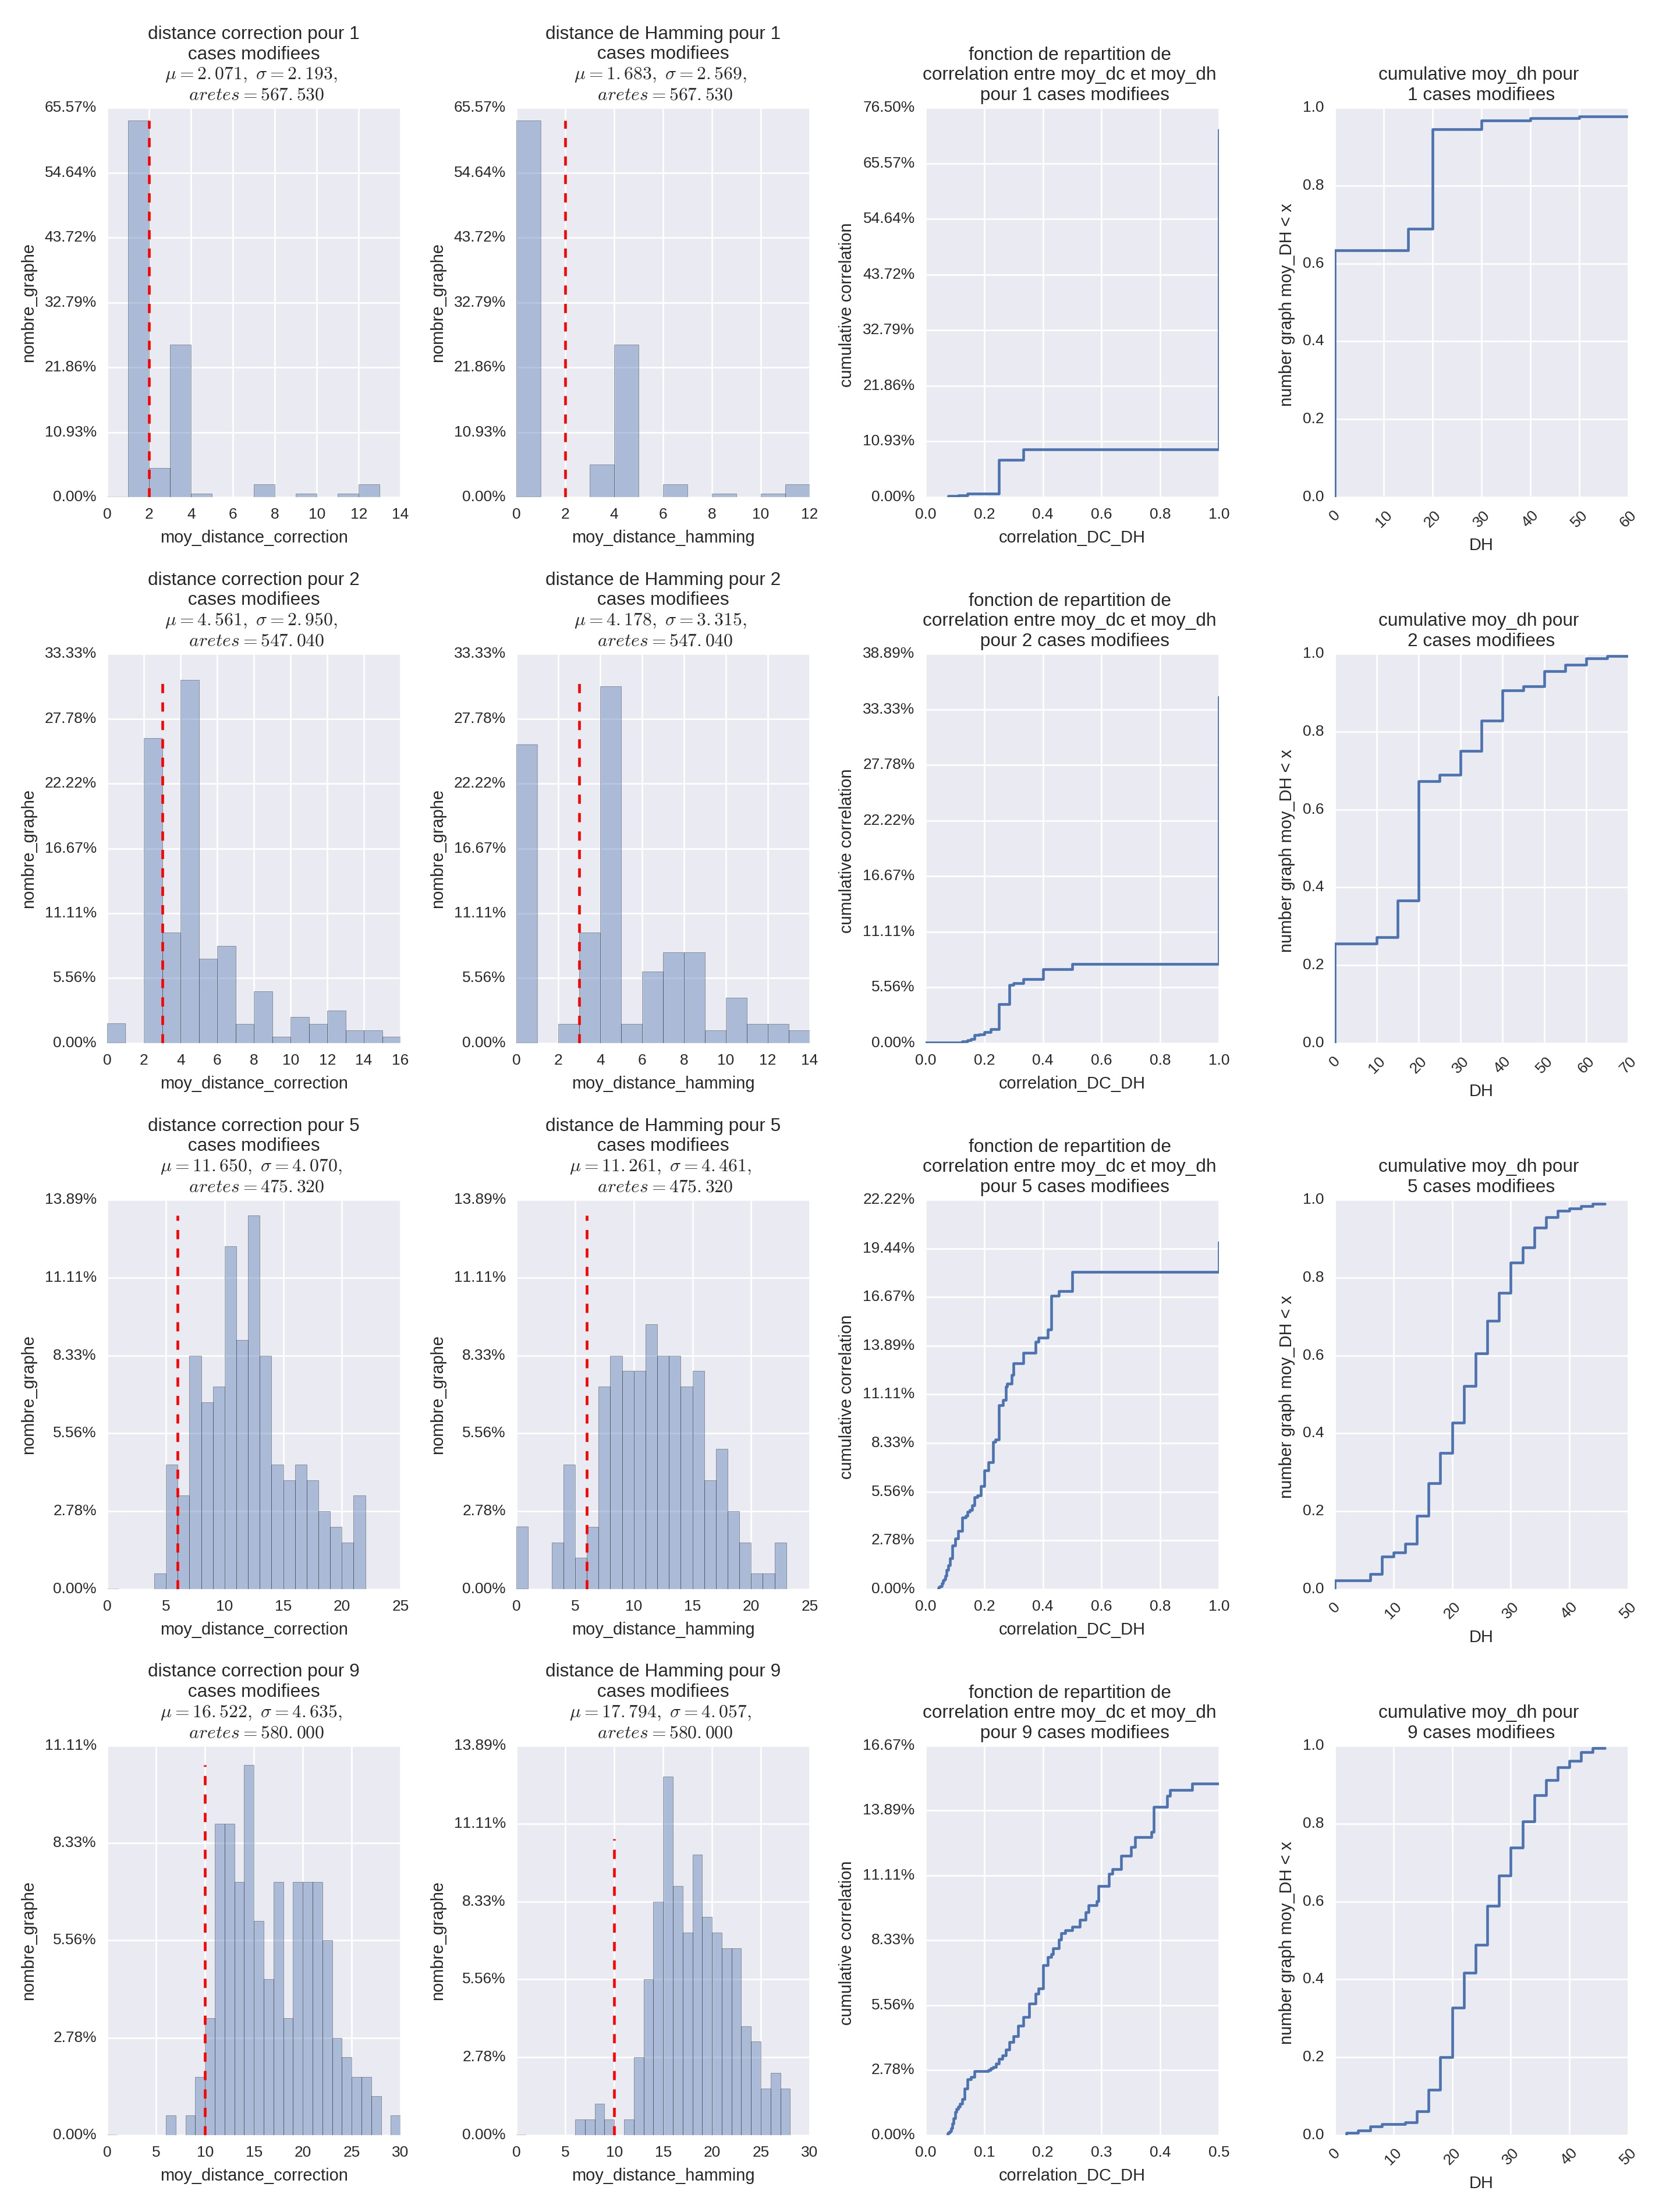
\includegraphics[width=550pt,height=570pt]{permut_distanceMoyenDLDH_k_1_2_5_9_aleatoire_p_05.jpeg}
\caption{ Approche de correction al\'eatoire sans remise \`a co\^ut unitaire pour $k =\{1,2,5,9\} $ cases modifi\'ees :
 La premi\`ere colonne repr\'esente la distribution des distances de correction $moy\_DC_{k,0.5}$. La seconde colonne est la distribution des distances de Hamming $moy\_DH_{k,0.5}$. 
 La troisi\`eme colonne  est la fonction de repartition de la corr\'elation entre les distances de correction et de Hamming avec en abscisse la corr\'elation entre ces distances (correlation\_DC\_DH).  
 La quatri\`eme colonne est la fonction cumulative des distances de Hamming. 
 La premi\`ere ligne est associ\'ee \`a $k=1$ case modifi\'ee, 
 la seconde ligne \`a $k=2$ cases modifi\'ees, 
 la troisi\`eme ligne \`a $5$ cases modifi\'ees et enfin 
 la derni\`ere \`a $9$ cases modifi\'ees.
 }
\label{sansremise_unitaire_distanceMoyenDCDH_k_1_2_5_9_aleatoire_p_05} 
\end{figure}
\FloatBarrier
% ----------------- figure permut_distanceMoyenDLDH_k_1_2_5_9_aleatoire_p_05 ---------------------

% k = 5
Pour $k = 5$, le pic se trouve toujours dans la zone {\em am\'eliorante} des colonnes $1$ et $2$ de la figure \ref{sansremise_unitaire_distanceMoyenDCDH_k_1_2_5_9_aleatoire_p_05} mais son pourcentage baisse significativement \`a $15.69\%$ (voir la ligne $3$). 
Le nombre de  line-graphes dans la zone {\em d\'egradante} dans les colonnes $1$ et $2$ augmente tout comme les distances de correction et de Hamming qui atteignent  jusqu'\`a $45$ ar\^etes.
La variable $\eta_k$ est \'egale \`a  $18.38\%$ de line-graphes $LG_{k,p,\alpha}$ (voir ligne $3$ de la colonne $3$ de la figure \ref{sansremise_unitaire_distanceMoyenDCDH_k_1_2_5_9_aleatoire_p_05}).
Cette augmentation provient de la baisse du pourcentage du pic de la zone {\em am\'eliorante} au profit de la zone {\em d\'egradante} et la plupart des graphes appartenant \`a cette zone ont leurs distances de correction et de Hamming corr\'el\'ees.
Les $15.69\%$  de line-graphes $LG_{k,p,\alpha}$ identiques \`a $LG$ s'expliquent par le type de cases modifi\'ees et l'emplacement des ar\^etes dans le graphe $LG$.  En effet, ces cases modifi\'ees sont des {\em fausses n\'egatives} et ces ar\^etes supprim\'ees n'appartiennent pas \`a des cliques voisines. Toutefois, quelque soit le type de cases modifi\'ees, notre couple d'algorithmes ajoutent beaucoup d'ar\^etes pour obtenir le line-graphe $LG_{k,p,\alpha}$ lorsque les cases sont reparties avec $p = 0.5$. Par exemple, nous avons constat\'e, en moyenne, $10$ \`a $20$ ar\^etes diff\'erentes pour $k=5$ cases modifi\'ees dans nos exp\'erimentations. 
Par ailleurs, nous remarquons qu'il existe des graphes dans lesquels la distance de correction est inf\'erieure \`a $k$. Tel est le cas pour $k = 5$ ou nous avons $moy\_DC_{k,0.5} = 3$ et $nombre\_graphe = 0.14\%$ dans la colonne $1$  de la figure \ref{sansremise_unitaire_distanceMoyenDCDH_k_1_2_5_9_aleatoire_p_05}.
En effet, les cases modifi\'ees sont des cases {\em fausses n\'egatives}. Ces ar\^etes supprim\'ees de $LG$ appartiennent \`a la m\^eme clique et certaines ar\^etes sont ajout\'ees de telle sorte que la clique se partitionne en deux cliques.   
%les aretes appartiennent a une meme cliques  de tel sorte qu'il ajoute certains aretes qui sindent la clique en deux cliques
%1) lalgo ajoute des aretes
%2) ces aretes  appartiennent a la meme clique et elles sont ajoutes de tel sorte que il forme deux cliques
\newline 

% k = 9
Enfin, pour $k=9$, la distribution des valeurs de distances est dans la zone {\em d\'egradante} et le pic est \`a $moy\_DC_{k,0.5} = 23$ cases modifi\'ees avec un pourcentage de $6\%$ line-graphes.  
En comparant les pourcentages des distances $moy\_DC_{k,0.5}$ et $moy\_DH_{k,0.5}$, nous constatons qu'ils ne sont pas identiques comme pour $k \le 5$. En effet, certaines cases modifi\'ees ne sont pas corrig\'ees car l'algorithme de correction modifie \'enorm\'ement de cases qui sont diff\'erentes des $k$ cases et ce taux croit quand  $moy\_DC_{k,0.5}$ est \'elev\'e. 
Le taux de cases corrig\'ees est de $53.38\%$ en moyenne.
La variable $\eta_k$ passe \`a $22\%$ de line-graphes $LG_{k,p,\alpha}$ parce que la correction a modifi\'ee des cases diff\'erentes des $k$ cases. Cependant les distances de correction et de Hamming restent toujours corr\'el\'ees et $3\%$ line-graphes $LG_{k,p,\alpha}$ ont le m\^eme ensemble d'ar\^etes que $LG$ (voir ligne $4$ de la colonne $3$ de la figure \ref{sansremise_unitaire_distanceMoyenDCDH_k_1_2_5_9_aleatoire_p_05}).
C'est pourquoi, les courbes de  $F_k(x)$ et $y_{cumulDH}^{k}$ ont cette forme enrob\'ee proche de la fonction  sigmoide de param\`etre $\lambda \le -15$. Pour rappel, nous pr\'ecisons que ces courbes  tendent vers la fonction suivante $f_{\lambda}(x) = \frac{1}{1+e^{\lambda * (x-0.5)}}$.
\newline
Les  cases modifi\'ees $k \in \{1,\cdots,9\}$ sont pr\'esent\'ees dans les figures 
 \ref{sansremise_unitaire_distanceMoyenDCDH_k_1_5_aleatoire_p_05} et  
\ref{sansremise_unitaire_distanceMoyenDCDH_k_6_9_aleatoire_p_05} de l'annexe \ref{annexe_distribution_0_9}.
\newline
% fin explication mode aleatoire sans remise avec cout unitaire 

L'approche de correction $(2c)$ nous montre que les distances de correction et de Hamming se d\'egradent quand le nombre $k$ de cases modifi\'ees augmentent. En fait, pour $k \le 5$, le nombre de line-graphes $LG_{k,p,\alpha}$ identiques \`a $LG$ est sup\'erieur \`a $nombre\_graphe = 25\%$ avec des distances de correction $moy\_DC_{k,0.5} = k$. Pour des distances $moy\_DC_{k,0.5} = 2 \times k$, les  $k$ cases modifi\'ees sont corrig\'ees. 
Des cases erron\'ees sont ajout\'ees pendant l'ex\'ecution de l'algorithme de correction mais elles sont peu nombreuses. Nous pouvons consid\'erer ces cases comme la pr\'ecision de notre algorithme  car ces cases indiquent le nombre de cases \`a modifier pour obtenir $LG$. Ainsi la distance de correction est major\'ee par le nombre de cases $k$ modifi\'ees.
Cependant, au d\'el\`a de $k > 5$,  la distance de correction $moy\_DC_{k,0.5}$ double et moins de $50\%$ des $k$ cases sont corrig\'ees. Les cases erron\'ees proviennent de l'ajout et la suppression d'ar\^etes dans le line-graphe $LG'_{k,p,\alpha}$ \'etant donn\'ee que la fonction de co\^ut est {\em unitaire}. La distance de correction est major\'ee par $2 \times k$ en moyenne.
\newline

{\bf Conclusion} : l'approche de correction {\em al\'eatoire sans remise} $(2c)$ propose des line-graphes $LG_{k,p}$  identiques \`a $LG$ quand $k \le 5$. Dans ce cas, le probl\`eme {\em Proxi-Line} est trait\'e car la distance line est major\'ee par $k$. 
Toutefois, le nombre de cases \`a corriger apr\`es l'ex\'ecution de notre couple d'algorithmes est faible lorsque la distance de correction est inf\'erieure au double de $k$ ($moy\_DC_{k,0.5} = 2 \times k$) avec $k>5$. Cela conduit \`a majorer la distance line par le double des cases erron\'ees.
En outre, pour $k>5$, le pourcentage  $\eta_k$ de corr\'elation entre $moy\_DC_{k,0.5}$ et $moy\_DH_{k,0.5}$ croit. Nous allons \'etudier l'\'evolution de $\eta_k$  dans le paragraphe \ref{relationMoyDHmoyDC} mais nous commencons par la comparaison des diff\'erentes approches de correction pour en d\'eduire celle qui minimise les distances de correction ou de Hamming.


		\subsubsection{Comparaison des modes de correction}
			
Nous recherchons la meilleure approche de correction parmi les cinq  \'enum\'er\'ees dans le tableau \ref{tab:recapApprocheCorrection}.
Pour ce faire, nous disposons des distributions des distances de correction et de Hamming, des fonctions de repartition de ces distributions et aussi des moyennes de distances de correction et de Hamming associ\'ees aux $k$ cases modifi\'ees. Les distributions des distances de correction et de Hamming sont obtenues avec  $p=0.5$ et la fonction de co\^ut est {\em unitaire}.
Les distributions de distances de chaque approche sont regroup\'ees dans les colonnes $1$ et $2$ dans les figures en annexes \ref{annexe_distribution_0_9}.
%Nous avons montr\'e dans le paragraphe \ref{relationMoyDHmoyDL} que la distance line peut \^etre utilis\'ee comme m\'etrique de comparaison entre deux graphes. Cependant, 
Nous d\'ecidons d'utiliser la moyenne des distances de Hamming pour la comparaison de approches de correction parce qu'il est facile de d\'eterminer le nombre de cases modifi\'ees \'etant donn\'ee que nous connaissons les line-graphes $LG$ et $LG_{k,p}$. 
\newline

%ARRETER ICI
%
%Soit $G_{k,p,\alpha}^{i}$  le $i^{ieme}$  graphe g\'en\'er\'e contenant $k$ cases modifi\'ees la $\alpha^{ieme}$ fois avec la repartition $p=0.5$ des $k$ cases. Nous le notons $G_{k,\alpha}^{i}$ avec $ 0 \le i \le 500$ et $\alpha \le \alpha_{max}$. \\
%Soit $DC_k^i$ le nombre de cases corrig\'ees par l'algorithme de correction pour le graphe $G_{k,\alpha}^{i}$.\\
%$\bar{DC_k^i}$ est la moyenne de $DC_k^i$ pour les $\alpha_{max}$ graphes $G_{k,\alpha}^{i}$.\\ 
%$\bar{DC_k}$ est la moyenne de $\bar{DC_k^i}$ pour $500$ graphes contenant $k$ cases modifi\'ees.\\
%Nous choisissons $\bar{DC_k}$ comme crit\`ere de comparaison des approches de corrections. %parce que A TROUVER 
%\newline
Soit $G_{k,p,\alpha}^{i}$  le $i^{ieme}$  graphe g\'en\'er\'e contenant $k$ cases modifi\'ees la $\alpha^{ieme}$ fois avec la repartition $p=0.5$ des $k$ cases. Nous le notons $G_{k,\alpha}^{i}$ avec $ 0 \le i \le 500$ et $\alpha \le \alpha_{max}$. Le line-graphe de  $G_{k,\alpha}^{i}$ obtenu apr\`es l'algorithme de correction est not\'e $L(G_{k,\alpha}^{i})$. \\
Soit $DH_k^i$ la distance de Hamming entre $LG$ et $L(G_{k,\alpha}^{i})$.  \\
La variable $moy\_DH_{k}^{i}$ est la moyenne de $DH_k^i$ pour les $\alpha_{max}$ graphes $G_{k,\alpha}^{i}$ et la variable $moy\_DH_{k}$ est la moyenne de $moy\_DH_{k}^{i}$ pour $500$ graphes contenant $k$ cases modifi\'ees.
La figure \ref{compareDifferentesMethodesCorrectionSommets_fct_cout_normal_p05} affiche les courbes  des diff\'erents approches de correction pour des distances de Hamming moyenn\'ees $moy\_DH_{k}$ en fonction des $k$ cases modifi\'ees. En ordonn\'e, nous avons le nombre de cases diff\'erentes entre deux line-graphes. 
\newline

% ----------- figure compareDifferentesMethodesCorrectionSommets _fct_cout_normal_p05 ----
%\vspace{-2.0cm}
\begin{figure}[htb!] 
\centering
% a changer par des chemins relatifs
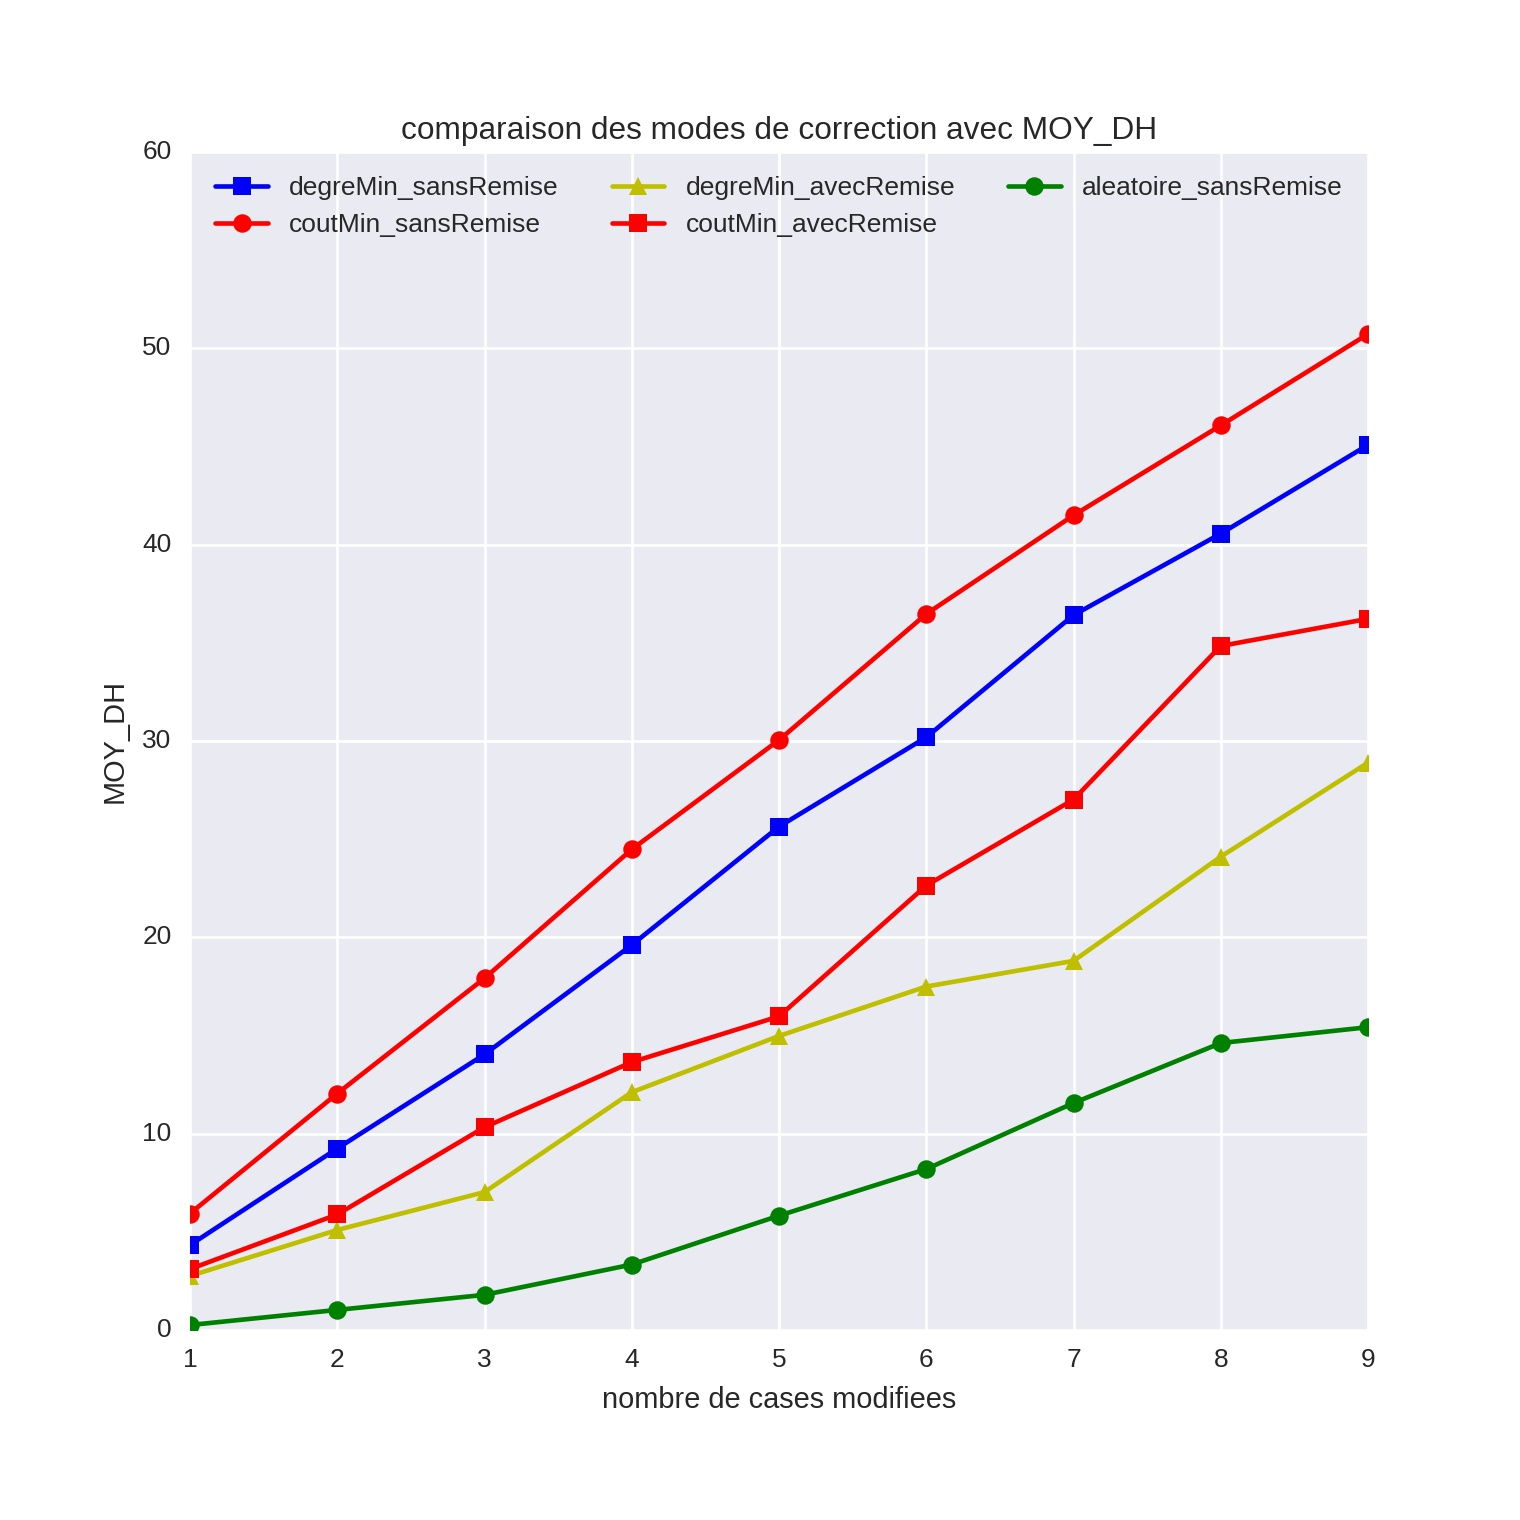
\includegraphics[scale=0.25]{simulation_comparaisonDifferentesMethodes_by_FonctDeCout_unitaire_500G_p_correl_05.jpeg}
\caption{ Comparaison des diff\'erentes approches de correction de sommets pour $k \in \{1,\cdots,9\}$ cases modifi\'ees. 
Les courbes en bleu carr\'e : approche degr\'e minimum sans remise (2a), 
			rouge carr\'ee : approche co\^ut minimum avec remise (1b), 
			rouge rond : approche co\^ut minimum sans remise (2b), 
			vert rond : approche al\'eatoire sans remise (2c) et 
			jaune triangle : approche degr\'e minimum avec remise (1a) 
}
\label{compareDifferentesMethodesCorrectionSommets_fct_cout_normal_p05} 
\end{figure}
\FloatBarrier
% ----------- figure compareDifferentesMethodesCorrectionSommets _fct_cout_normal_p05 ----


Consid\'erons des courbes associ\'ees aux approches $(2b)$, $(2c)$ et $(1b)$. 
En choisissant les nombres de cases modifi\'ees $k \in \{4, 8\}$, nous avons $moy\_DH_{k,p} \in \{4,15\}$ cases pour l'approche $(2c)$, $moy\_DH_{k,p} \in \{13, 36\}$ cases  pour l'approche $(1b)$ et $moy\_DH_{k,p} \in \{25, 46\}$ cases  pour l'approche $(2b)$.
Pour $k=4$ cases modifi\'ees, l'approche $(1b)$  modifie, en moyenne, $9$ cases de plus que l'approche $(2c)$. En revanche, ce nombre moyen de cases modifi\'ees augmente \`a $21$ cases quand $k=8$. 
De m\^eme, l'approche $(2b)$ modifie $12$ cases de plus que l'approche $(1b)$ pour $k=4$ cases modifi\'ees et $10$ cases pour $k=8$ cases.
L'approche  $(2c)$ donne de meilleures r\'esultats par rapport aux approches $(1b)$ et $(2b)$.
\newline


% conclusion
{\bf Conclusion} : l'approche {\em al\'eatoire sans remise} propose de meilleurs r\'esultats que les approches $(2a)$, $(2b)$, $(1a)$ et $(1b)$ parce que les distances de correction sont minimales pour toute valeur de $k$ comme le montre la figure \ref{compareDifferentesMethodesCorrectionSommets_fct_cout_normal_p05}.
Nous retenons, pour la suite,  l'approche {\em al\'eatoire sans remise}  comme l'approche de correction des sommets de $\cal C$, sommets n'appartenant \`a aucune couverture.
%D'autre part, ce r\'esultat a \'et\'e obtenu avec la fonction de co\^ut {\em unitaire}.




		\subsubsection{Influence des cases modifi\'ees et de la fonction de co\^ut}
			\label{influenceFonctionCoutDistributionHamming1}
			% ------------- comparaison_p_correl_s_aleatoire_aucune ----------
\begin{figure}[htb!] 
\centering
% aleatoire aucune = aleatoire unitaire
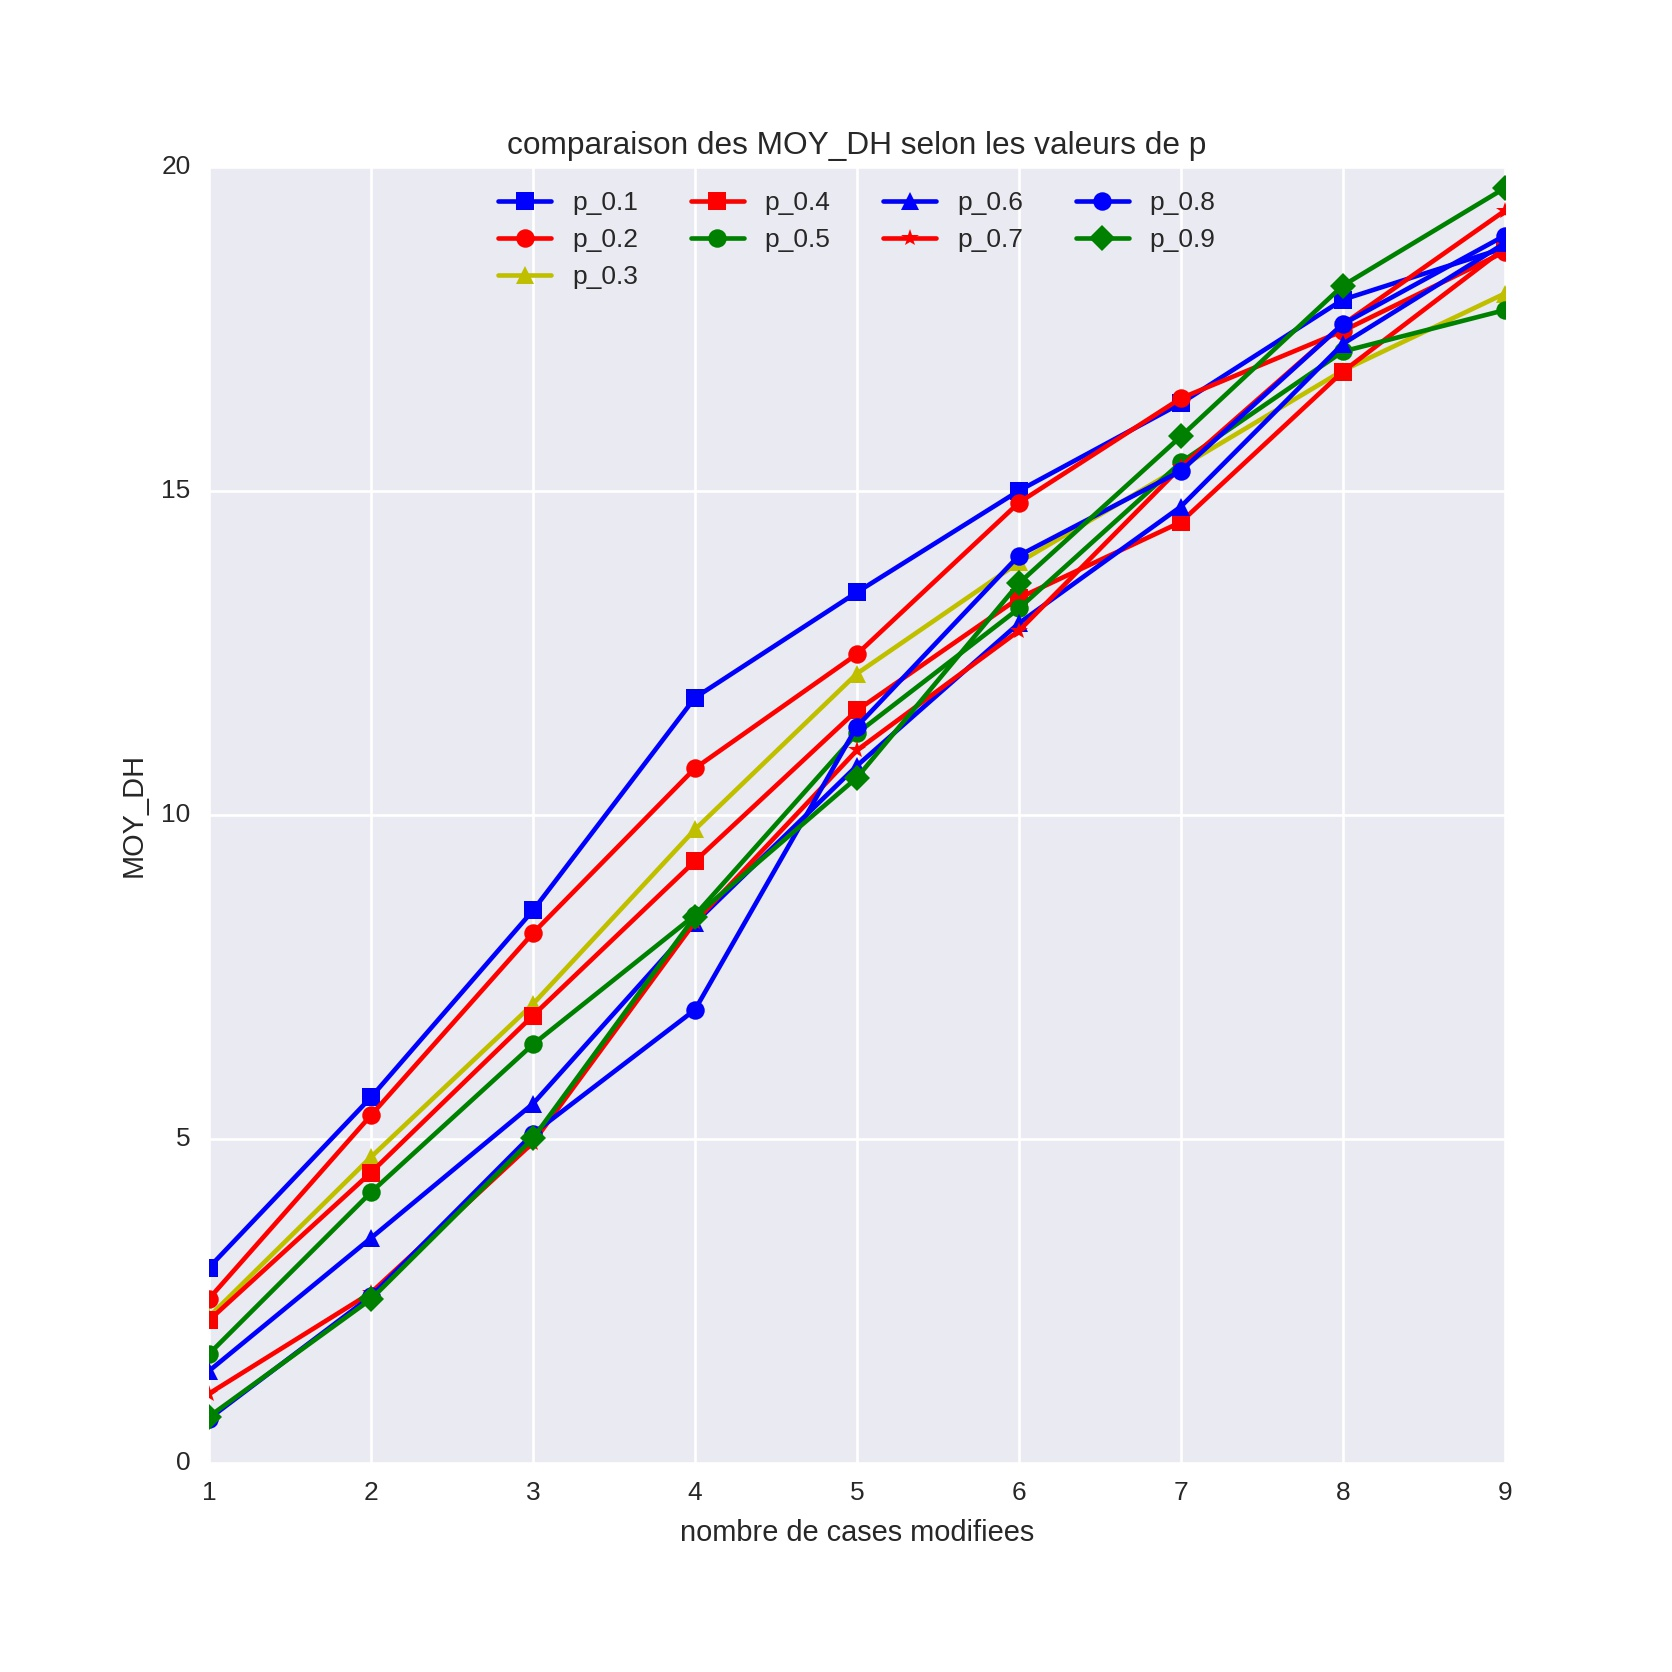
\includegraphics[scale=0.25]{comparaison_p_correl_s_aleatoire_aucune.jpeg}
\caption{ Comparaison des diff\'erentes repartitions des $k \in \{1,\cdots,9\}$ cases fausses positives et fausses n\'egatives avec l'approche {\em al\'eatoire sans remise} et la fonction de co\^ut {\em unitaire}. }
\label{comparaison_p_correl_s_aleatoire_aucune} 
\end{figure}
%\FloatBarrier
% ------------- comparaison_p_correl_s_aleatoire_aucune ----------


Nous mesurons l'influence des fonctions de co\^ut sur nos distances de Hamming.
Pour ce faire, nous appliquons les fonctions de co\^ut {\em unitaire}, {\em ajout} et {\em suppression} (voir tableau \ref{tab:recapApprocheCorrection}) pour en d\'eduire les valeurs de $p$ qui sont favorables \`a l'algorithme de correction c'est-\`a-dire qui minimisent les distances de Hamming.
\newline

Nous consid\'erons d'abord la fonction {\em unitaire}.
La figure \ref{comparaison_p_correl_s_aleatoire_aucune} repr\'esente l'\'evolution des distances de Hamming selon les diff\'erentes valeurs de $p$.  Les courbes de $p$ sont \'eloign\'ees pour $k \le 5$ et au d\'el\`a de  $k > 5$, les courbes se rapprochent. 
En effet, 
pour $k \le 5$, $43.4\%$ des cases {\em fausses n\'egatives} en moyenne sont corrig\'ees pour $p\in \{0.7, 0.9\}$ et pour $p=0.8$, cette moyenne est de $45.5\%$. Quant aux cases {\em fausses positives}, seulement $10\%$ des cases sont corrig\'ees. 
Ces moyennes sont plus \'elev\'ees que celles obtenues avec $p<0.7$.  
En effet, seulement $19.32\%$ des cases {\em fausses positives} et $38\%$ des cases  {\em fausses n\'egatives} sont corrig\'ees avec  $p<0.7$. 
 L'algorithme de correction ajoute beaucoup d'ar\^etes pour $p \ge 0.7$ par rapport \`a $p<0.7$ parce que le nombre de cases {\em fausses n\'egatives} dans la matrice du graphe de corr\'elation est \'elev\'e pour $p<0.7$ sachant que le co\^ut d'ajout  d'une ar\^etes est de $1$.
\newline
De m\^eme, pour $k > 0.5$, $80\%$ des cases erron\'ees sont des cases {\em fausses n\'egatives} apr\`es l'algorithme de correction.  L'algorithme privil\'egie l'ajout  \`a la suppression d'ar\^etes. 
\newline
La fonction {\em unitaire} a peu d'influence sur les variations des distances de Hamming quelque soit les valeurs de $p$.  

% ------------- comparaison_p_correl_s_aleatoire_ajout -----------
\begin{figure}[htb!] 
\centering
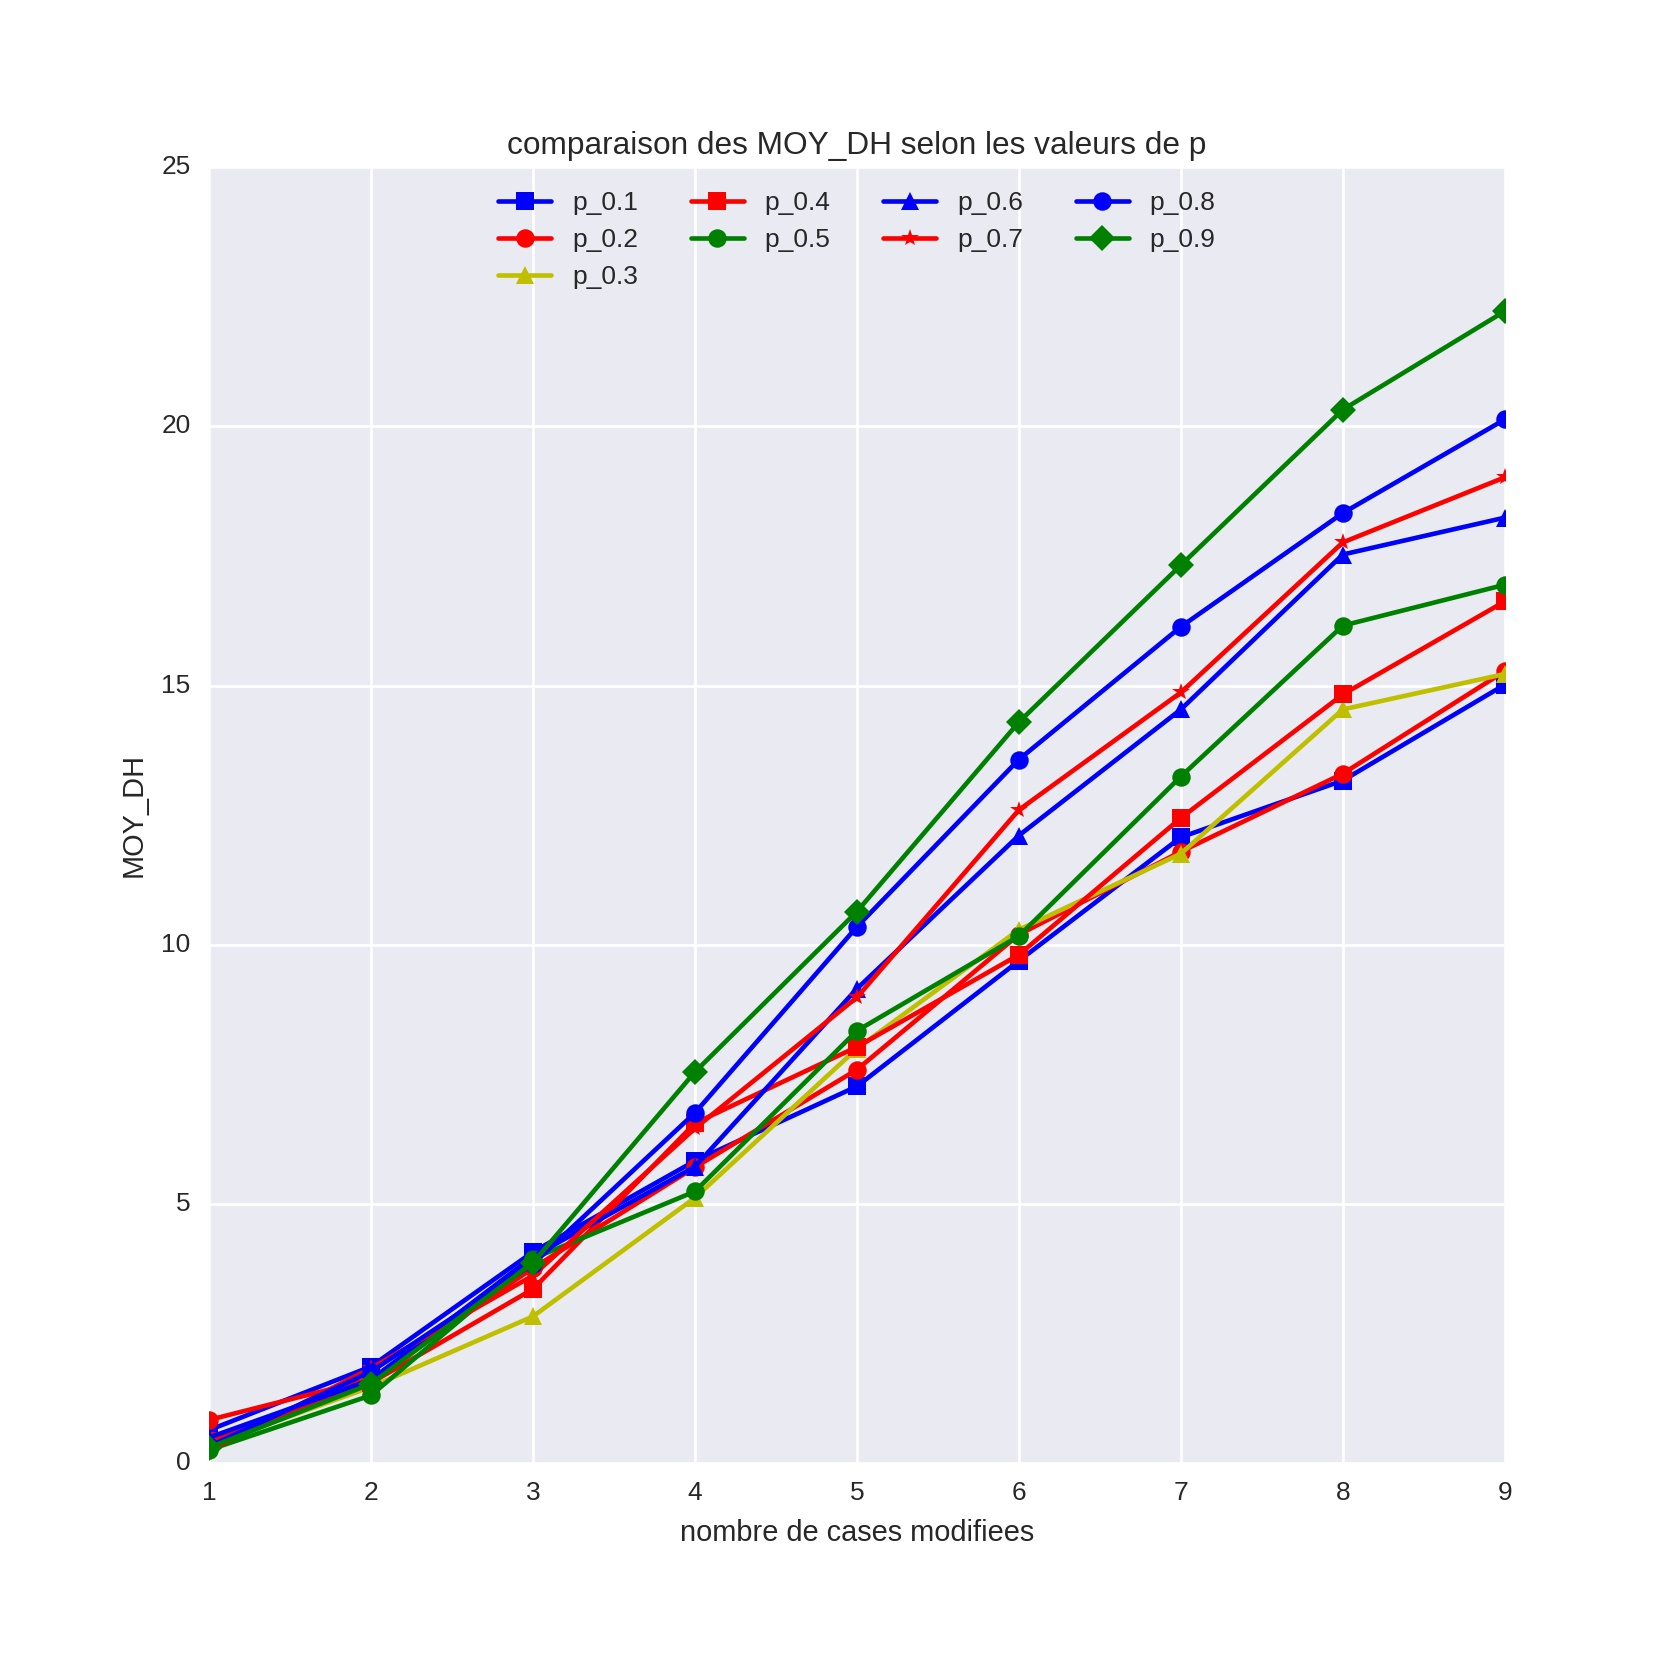
\includegraphics[scale=0.25]{comparaison_p_correl_s_aleatoire_ajout.jpeg}
\caption{ Comparaison des diff\'erentes repartitions des $k \in \{1,\cdots,9\}$ cases fausses positives et fausses n\'egatives avec l'approche {\em al\'eatoire sans remise} et la fonction de co\^ut {\em ajout}.  }
\label{comparaison_p_correl_s_aleatoire_ajout} 
\end{figure}
%\FloatBarrier
% ------------- comparaison_p_correl_s_aleatoire_ajout -----------

La figure \ref{comparaison_p_correl_s_aleatoire_supp} correspond \`a la fonction {\em suppression} et elle a le m\^eme comportement que la fonction {\em unitaire} parce que toutes les courbes divergent quand $k \le 5$ et convergent quand  $k > 5$. Ici nous remarquons aussi que nous avons en moyenne beaucoup de cases {\em fausses n\'egatives} en moyenne \`a la fin de l'algorithme de correction. 
Avec la fonction {\em suppression}, nous constatons que le nombre moyen de cases {\em fausses n\'egatives} \`a la fin de l'algorithme de correction est largement sup\'erieur au nombre de cases {\em fausses n\'egatives} modifi\'ees dans la matrice $M_{k,p,\alpha}$.
Cependant, le nombre de ces cases {\em fausses n\'egatives}  ($39.4\%$ en moyenne) \`a la fin de l'algorithme de correction est inf\'erieur au nombre de cases corrig\'es {\em fausses n\'egatives}  ($47.7\%$ en moyenne) avec la fonction {\em unitaire}. 
Cette baisse provient majoritairement de la position des sommets \`a corriger dans ${\cal C}$. 
En effet, il existe des chaines simples de longueur $2$ entre certains sommets de  ${\cal C}$.  Une ar\^ete de chacune des chaines est supprim\'ee afin que la compression de deux cliques fournisse une nouvelle clique de ${\cal CC}$. Cela fait que les ar\^etes incidentes ont leurs sommets de ${\cal CC}$ et ces ar\^etes sont supprim\'ees une fois sur deux au minimum. 
La fonction {\em suppression} donne le m\^eme r\'esultat que la fonction {\em unitaire}.
%\newline

% ------------- comparaison_p_correl_s_aleatoire_supp  ----------
\begin{figure}[htb!] 
\centering
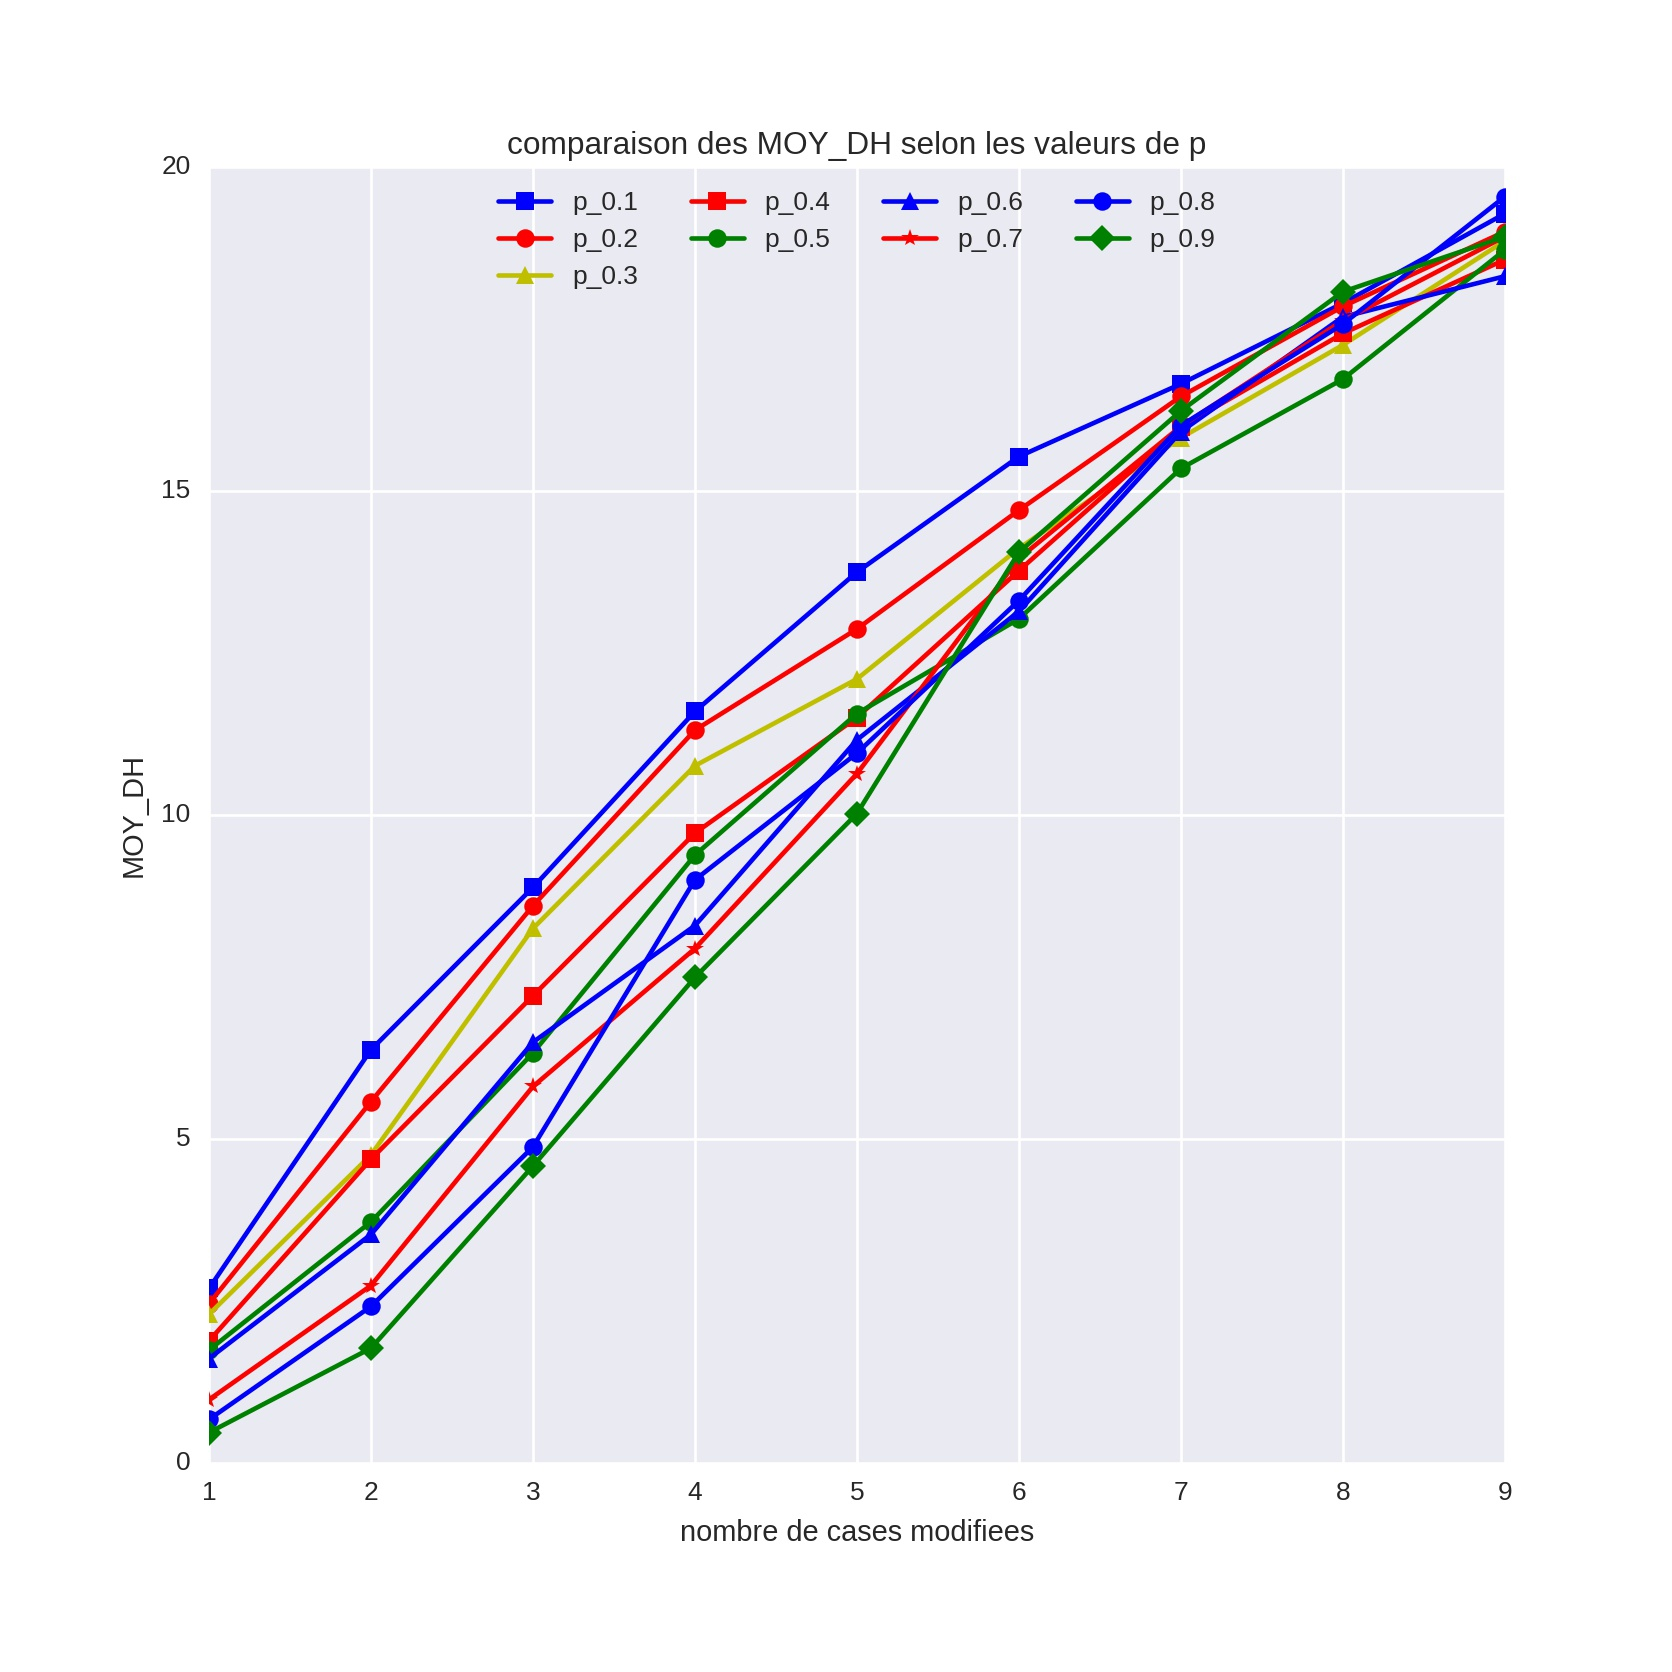
\includegraphics[scale=0.25]{comparaison_p_correl_s_aleatoire_supp.jpeg}
\caption{ Comparaison des diff\'erentes repartitions des $k \in \{1,\cdots,9\}$ cases fausses positives et fausses n\'egatives avec l'approche {\em al\'eatoire sans remise} et la fonction de co\^ut {\em suppression}. }
\label{comparaison_p_correl_s_aleatoire_supp} 
\end{figure}
%\FloatBarrier
% ------------- comparaison_p_correl_s_aleatoire_supp  ----------

Dans la figure \ref{comparaison_p_correl_s_aleatoire_ajout} associ\'ee \`a la fonction {\em ajout}, les courbes divergent quand $k$ est croissant.
En effet, des ar\^etes {\em fausses n\'egatives}  sont ajout\'ees \`a $G_{k,p,\alpha}$ pour $p \ge 0.4$ pendant la correction. Alors les distances $moy\_DH_{k,p}$ augmentent car le nombre de cases  {\em fausses n\'egatives} augmente et aussi plus de  $40\%$ des cases {\em fausses positives} ne sont pas supprim\'ees.  
Par ailleurs, les courbes convergent vers $0$ quand $k \le 4$. La baisse des valeurs moyennes des distances de Hamming est le r\'esultat de la correction des cases modifi\'ees dans $M_{k,p}$. N\'eanmoins, l'algorithme corrige majoritairement des cases {\em fausses n\'egatives} lorsque toutes les cases modifi\'ees ne parviennent pas \`a \^etre corrig\'ees. 
\newline

{\bf Conclusion} : nous ne pouvons pas conclure que les valeurs de $p$ ont une influence sur la correction des $k$ cases modifi\'ees car les fonctions de co\^ut {\em unitaire} et {\em suppression} font converger l'une vers l'autre leurs distances de Hamming avec l'augmentation du nombre de cases modifi\'ees. Toutefois, la fonction de co\^ut {\em ajout} fait diverger nos courbes sans cr\'eer un \'ecart significatif de distances entre ses courbes. 



%
%Consid\'erons $p \in [0,1]$, la variable de repartition des $k$ cases modifi\'ees. 
%$p = 0.1$ signifie que $10\%$ des $k$  cases modifi\'ees ajoutent des ar\^etes au graphe  $G_{k,p, \alpha}$ (cases {\em fausses positives}) et les $90\%$ des cases restantes suppriment des ar\^etes du graphe (cases {\em fausses n\'egatives}). Nous pr\'ecisons \'egalement que la fonction de co\^ut est {\em unitaire}.
%La figure \ref{comparaison_p_correl_s_aleatoire_aucune} r\'esume 
%l'\'evolution des distances de Hamming $moy\_DH$ en fonction des $k \in \{1,\cdots,9\}$ cases modifi\'ees pour diff\'erentes valeurs de $p$. 
%Les courbes sont croissantes et  la courbe de $p = 0.8$ donne les distances de Hamming minimales  \`a partir de $k \le 4 $. Au d\'el\`a de $k > 4$, les courbes se rapprochent les unes des autres et il est difficile de d\'eterminer la valeur $p$ qui fournit la plus petite distance.
%En effet, pour  $k \le 4$, les courbes divergent parce que les cases modifi\'ees ne sont pas corrig\'ees et d'autres cases sont modifi\'ees. Cela augmente l'ensemble de cases ({\em fausses n\'egatives et fausses positives}).
%N\'eammoins, les cases modifi\'ees sont corrig\'ees pour $k > 4$ et cela entraine que les courbes se rapprochent.
%Le probl\`eme de la bonne repartition semble \^etre difficile \`a trouver pour la fonction de cout {\em unitaire}. Nous allons appliquer d'autres fonctions de co\^ut pour d\'eduire une valeur de $p$ acceptable qui minimise les distances de Hamming.
%\newline
%La fonction de co\^ut {\em suppression} a le m\^eme comportement que la fonction {\em unitaire} comme indiqu\'e dans la figure \ref{comparaison_p_correl_s_aleatoire_supp}. La divergence des courbes se produit pour $k \in \{1,\cdots,5\}$ et la courbe de $p = 0.9$ fournit les distances de Hamming minimales (sa courbe est en dessous des autres). \`A partir de $k > 5$, les courbes se rapprochent et la meilleure courbe est  celle de $p = 0.5$. 
%Nous l'expliquons par la modification des cases {\em fausses n\'egatives} pour $p =0.9$ et par  l'ajout d'ar\^etes pour $p = 0.5$.
%\newline
%Dans la figure \ref{comparaison_p_correl_s_aleatoire_ajout} associ\'ee \`a la fonction de co\^ut {\em ajout}, les courbes divergent quand $k$ est croissant.
%En effet, des ar\^etes suppl\'ementaires  sont ajout\'ees \`a $G_{k,p}$ pour $p \ge 0.4$. Les distances $moy\_DH$ augmentent car plus de  $40\%$ des cases {\em fausses positives} ne sont pas supprim\'ees.  
%Par ailleurs, pour $p = 0.1$, la distance de Hamming moyenne est de $1.421,2.305,3.109$ pour $k = 1,2,3$ respectivement et pour $k \ge 4$, cette distance augmente d'environ $1.5 \times k$.
%L'algorithme corrige autour de $20\%$ les cases {\em fausses n\'egatives} et les ar\^etes de la distance de Hamming correspondent majoritairement aux cases {\em fausses positives} modifi\'ees  pendant la phase de correction.
%\newline
%Nous ne pouvons pas conclure que la repartition des $k$ cases modifi\'ees de $M_{LG}$ a un impact sur la correction des sommets $noeud \in {\cal C}$ car les fonctions de co\^ut {\em unitaire} et {\em suppression} font converger nos distances de Hamming avec l'augmentation du nombre de cases modifi\'ees. Toutefois, la fonction de co\^ut {\em ajout} fait diverger nos courbes sans cr\'eer un \'ecart significatif de distances entre ses courbes.  


% ----- partir a envoyer 



%% comparaison de p_correl sur la methode de permutation aleatoire
%%% ---- pas encore REPROGRAMMER -- utiliser la fonction de cout unitaire
%\begin{figure}[htb!] 
%\centering
%% meilleur probabilite p parmi les [0.0, 0.1, 0.2, ...., 1.0]
%% a changer par des chemins relatifs
%%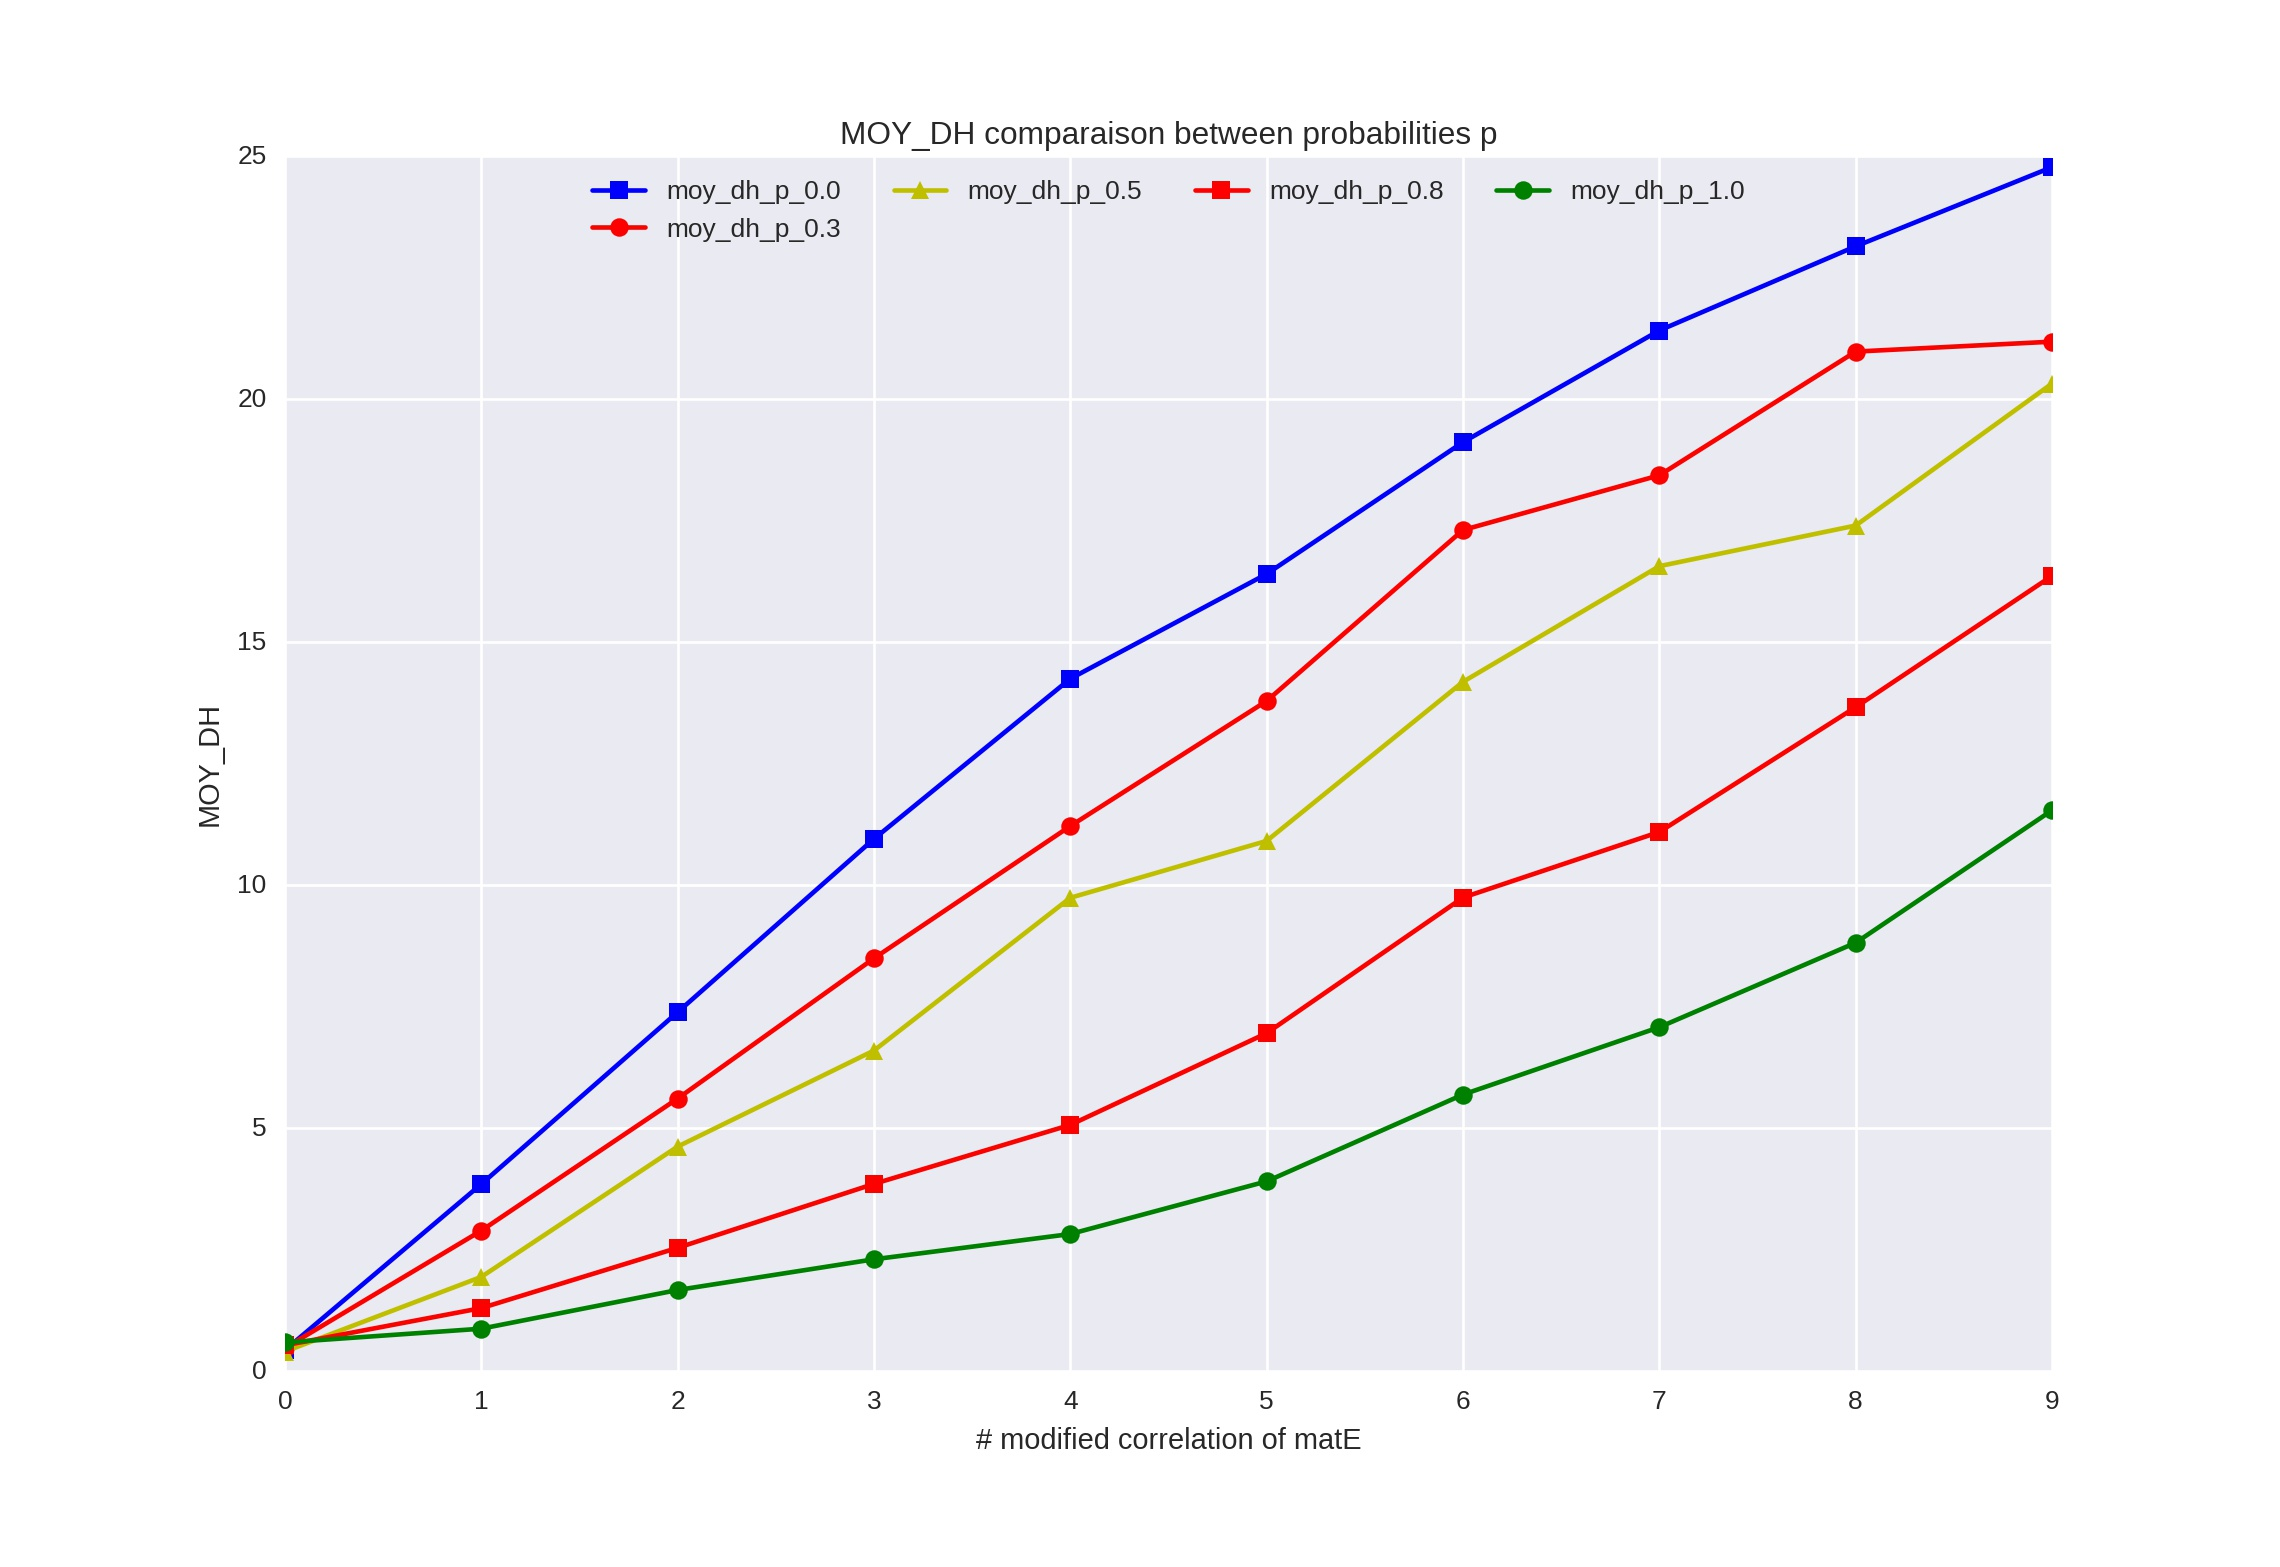
\includegraphics[scale=0.25]{permut_aleatoire_coutMin_degreMin_fct_cout_normal_500G/aleatoire/courbes/comparaison_probabilities_p_00_10_moy_dh_aleatoire_p_10.jpeg}
%%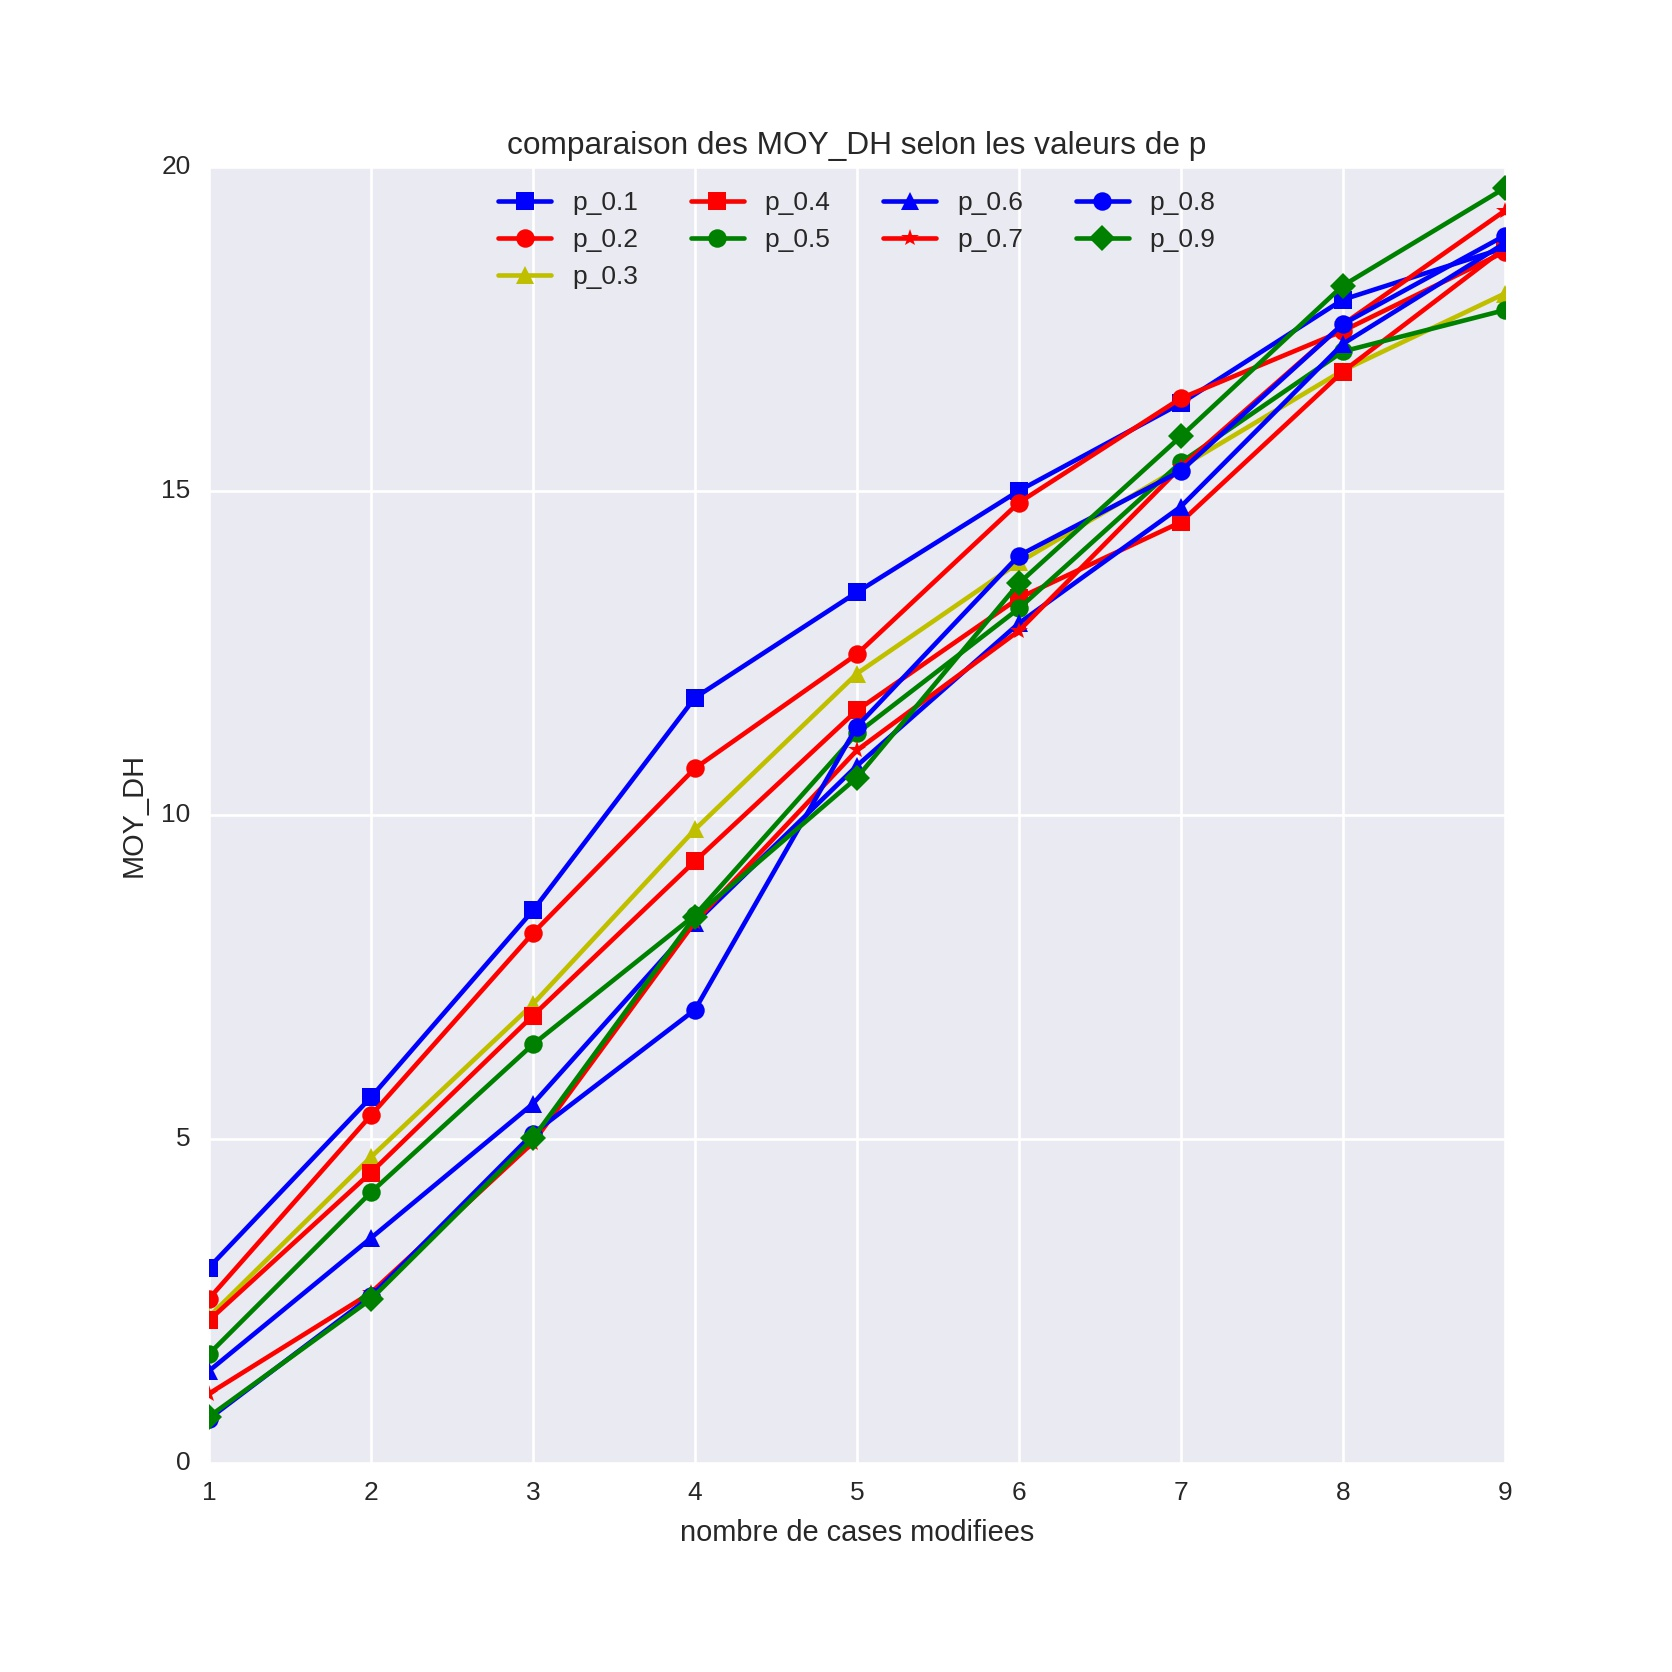
\includegraphics[scale=0.25]{comparaison_p_correl_s_aleatoire_aucune.jpeg}
%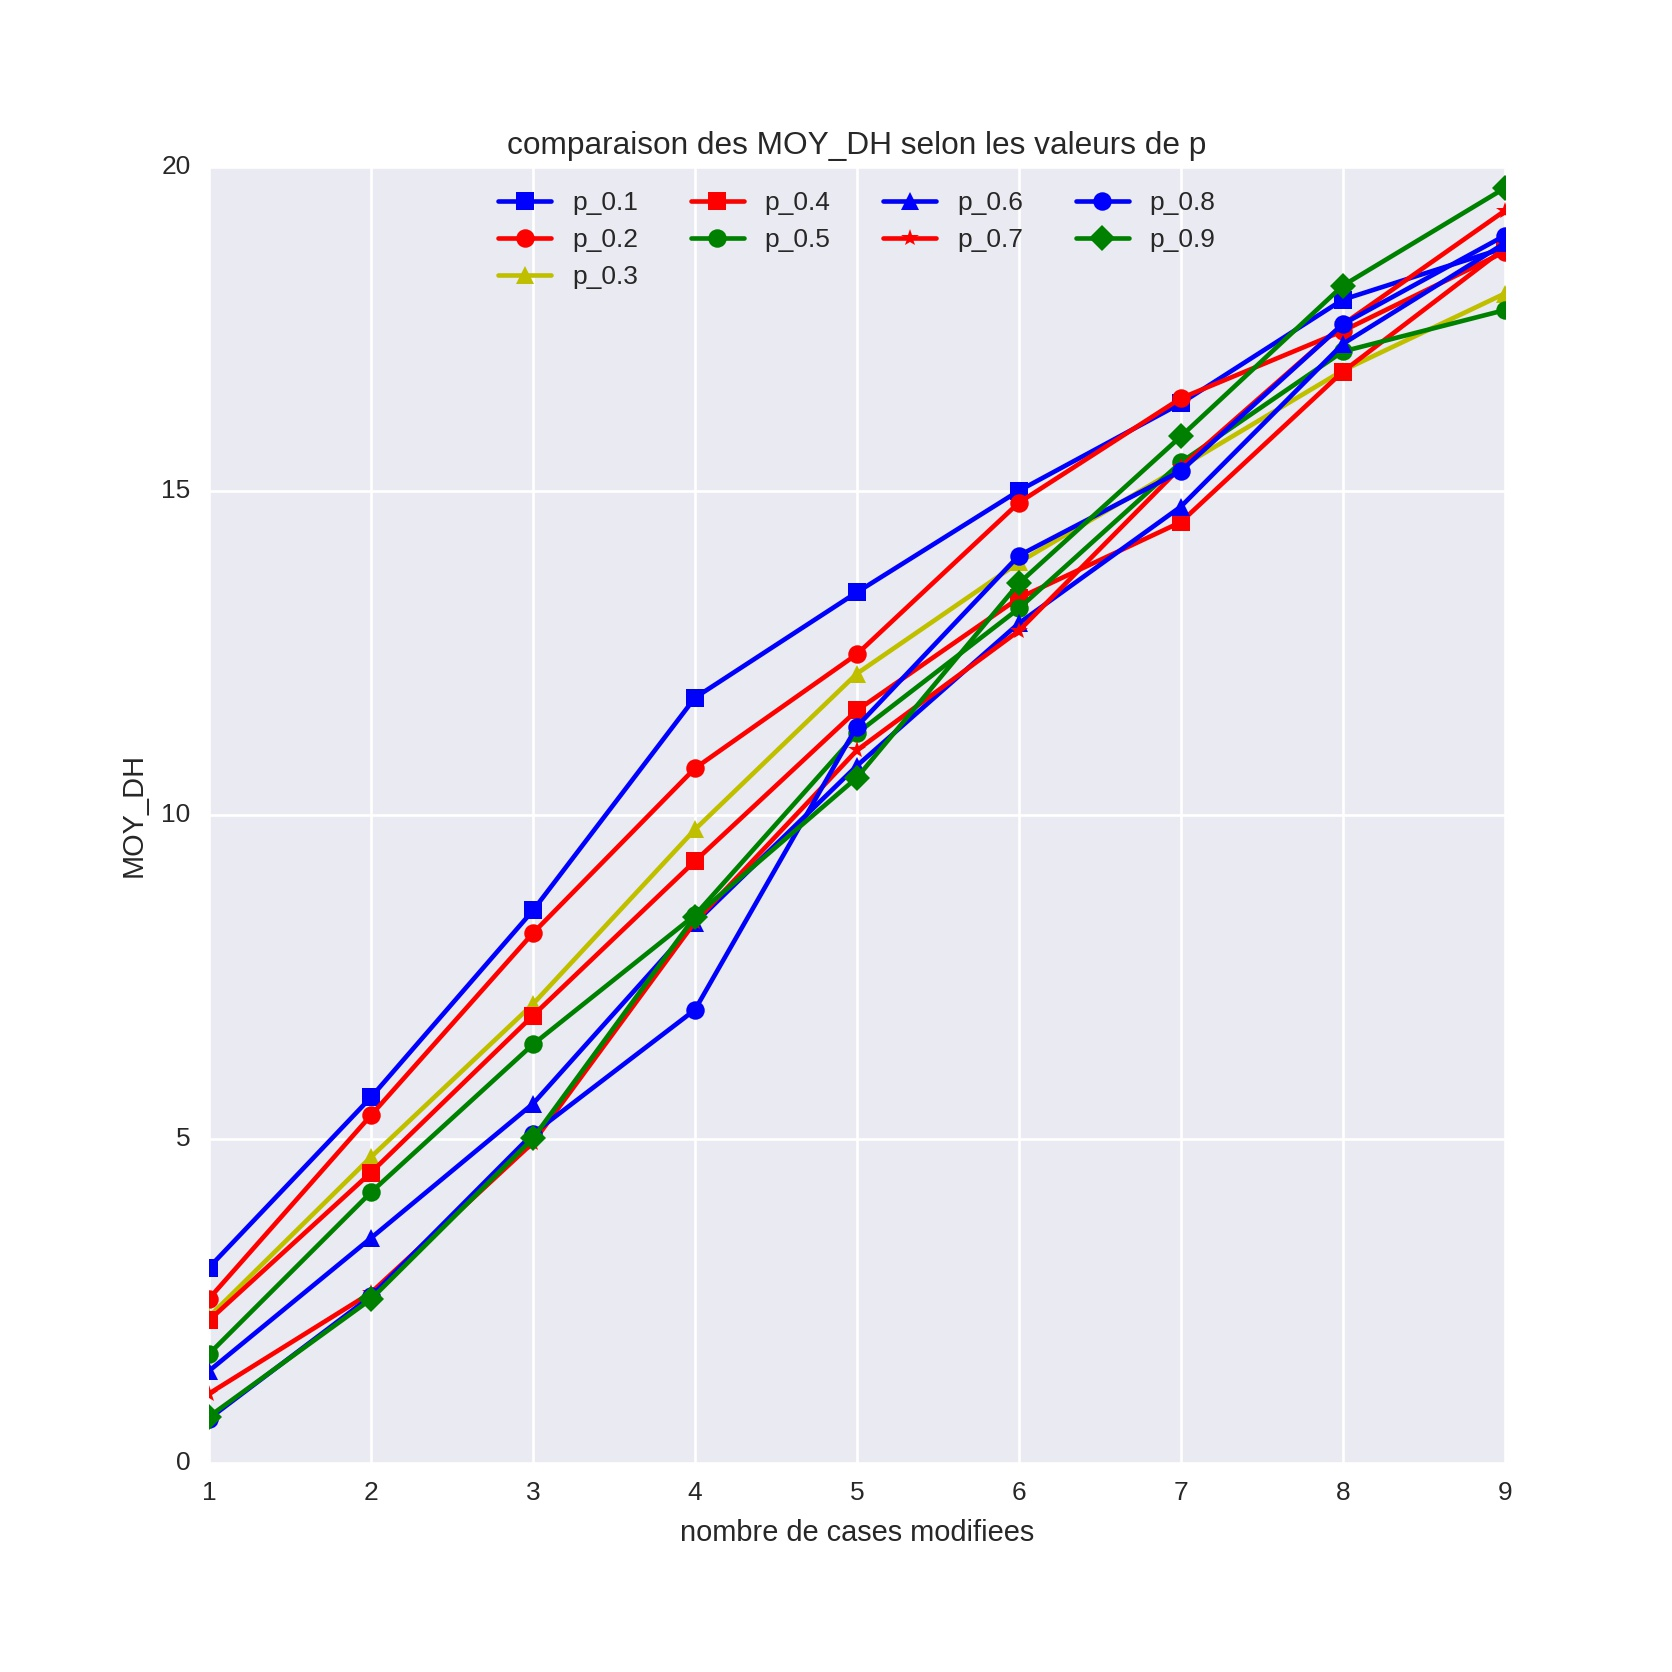
\includegraphics[scale=0.25]{comparaison_p_correl_s_aleatoire_aucune.jpeg}
%\caption{ Comparaison des diff\'erentes probabilit\'es d'ajout $k \in [1,9]$ de corr\'elations fausses positives et fausses n\'egatives sur la m\'ethode de permutation al\'eatoire }
%\label{comparaison_p_correl_s_aleatoire_aucune} 
%\end{figure}
%%% ---- pas encore REPROGRAMMER
%Consid\'erons la variable $p\_correl \in [0,1]$. 
%$p\_correl = 0.1$ signifie que $10\%$ des $k$  cases modifi\'ees ajoutent des ar\^etes au graphe  $G_{k,p\_correl, \alpha}$ (erreurs {\em fausses positives}) et les $90\%$ des cases restantes suppriment des ar\^etes du graphe (erreurs {\em fausses n\'egatives}). Nous pr\'ecisons \'egalement que  l'ajout et la suppression d'ar\^etes ont le m\^eme co\^ut de traitement c'est-\`a-dire $1$.
%La figure \ref{comparaison_p_correl_s_aleatoire_aucune} r\'esume 
%l'\'evolution des distances de Hamming $moy\_DH$ en fonction des $k \in [1,9]$ cases modifi\'ees pour diff\'erentes valeurs de $p\_correl$. 
%Les courbes sont croissantes et nous constatons que pour $k \le 4 $, la courbe de $p\_correl = 0.8$ donne les distances de Hamming minimales. Au d\'el\`a de $k > 4$, les courbes se rapprochent les unes des autres et il est difficile de determiner la valeur $p\_correl$ qui fournit la plus petite distance.
%En effet, La parit\'e de co\^uts n'impacte pas les d\'ecisions de l'algorithme de correction qui aura tendance \`a ajouter et supprimer des ar\^etes. Pour $k \le 4$, les courbes divergent parce que les cases modifi\'ees ne sont pas corrig\'ees et des erreurs sont ajout\'ees dans chaque ensemble d'erreurs ({\em fausses n\'egatives et fausses positives}). Ces erreurs sont soit l'ajout d'ar\^etes  dans les erreurs {\em fausses positives} ou soit la suppression d'ar\^etes dans les  erreurs {\em fausses n\'egatives}. Cependant, les courbes se rapprochent pour $k > 4$ car l'algorithme ajoute et supprime plusieurs fois les m\^emes ar\^etes. 
%%De m\^eme, le taux d'erreurs {\em vrai n\'egatives} et {\em fausses positives} restent stables dans l'ensemble    =====> A complter apres la courbe.
%Il nous est impossible d'affirmer la bonne repartition des $k$ cases dans le  cas {\em priorit\'e aucune}.
%\newline
%En changeant la {priorit\'e aucune} aux {\em priorit\'es ajout ou suppression}, parvenons nous \`a deduire une valeur de $p\_correl$ acceptable c'est-\`a-dire qui minimise les distances de Hamming? 
%% reste priorite suppression 
%\newline
%La {\em priorit\'e suppression} a le m\^eme comportement que la {\em priorit\'e aucune} comme indiqu\'e dans la figure \ref{comparaison_p_correl_s_aleatoire_supp}. La divergence des courbes se produit pour $k \in [1,5]$ avec la courbe de $p\_correl = 0.9$ fournissant les distance de Hamming minimales (sa courbe est en dessous des autres). \`A partir de $k > 5$, les courbes convergent et la meilleure courbe \'est  celle de $p\_correl = 0.5$. 
%\begin{figure}[htb!] 
%\centering
%%\includegraphics[scale=0.25]{comparaison_taux_vrai_negatifs_corriges_p_correl_s_aleatoire_supp.jpeg}
%\caption{ Taux d'erreurs fausses negatives corrig\'ees pour $k \in [1,9]$ cases modif\'ees et une m\'ethode de corr\'elation al\'eatoire avec la priorit\'e suppression}
%\label{comparaison_taux_vrai_negatifs_corriges_p_correl_s_aleatoire_supp} 
%\end{figure}
%Nous l'expliquons par la suppression des erreurs {\em fausses n\'egatives} (voir figures \ref{comparaison_taux_vrai_negatifs_corriges_p_correl_s_aleatoire_supp}) pour $p_correl =0.9$ et par  la correction des ar\^etes pour $p\_correl = 0.5$
%
%
%Dans la figure \ref{comparaison_p_correl_s_ajout} associ\'ee \`a la {\em priorit\'e ajout}, Les courbes divergent quand $k$ est croissant. {\bf Pourquoi?} En effet, l'algorithme de correction a tendance \`a ajouter des ar\^etes dans le voisinage des sommets \`a corriger. Cela entraine des ar\^etes suppl\'ementaires qui augmentent la distance de Hamming pour les valeurs de $p\_correl \ge 0.4$, \'etant donn\'ee que plus de $40\%$ des erreurs {\em fausses positives} ne sont pas supprim\'ees.  
%Par ailleurs, pour $p\_correl = 0.1$, la distance de Hamming moyenne est de $1.421,2.305,3.109$ pour $k = 1,2,3$ respectivement et pour $k \ge 4$, cette distance augmente d'environ $1.5 * k$. L'algorithme corrige autour de $20\%$ les erreurs {\em fausses n\'egatives} et les ar\^etes diff\'erentes de la distance de Hamming correspondent aux erreurs {\em fausses positives} et majoritairement aux ar\^etes ajout\'ees de l'algorithme.
%Toutefois le taux d'ar\^etes corrig\'ees dans les erreurs {\em fausses n\'egatives} est tr\^es bas comme le montre la figure \ref{comparaison_taux_vrai_negatifs_corriges_p_correl_s_aleatoire_ajout}. 
%\begin{figure}[htb!] 
%\centering
%%\includegraphics[scale=0.25]{comparaison_taux_vrai_negatifs_corriges_p_correl_s_aleatoire_ajout.jpeg}
%\caption{ Taux d'erreurs fausses negatives corrig\'ees pour $k \in [1,9]$ cases modif\'ees et une m\'ethode de corr\'elation al\'eatoire avec la priorit\'e ajout}
%\label{comparaison_taux_vrai_negatifs_corriges_p_correl_s_aleatoire_ajout} 
%\end{figure}
%\newline
%Nous ne pouvons pas conclure que la repartition des $k$ cases modifi\'ees de $M_{LG}$ est un impact sur la correction des sommets $\in sommets\_1$ car notre algorithme a un defaut celui d'ajouter des ar\^etes et aussi le taux d'erreurs {\em fausses negatives} corrig\'es est tr\`es faible.
%%Cette valeur $p\_correl = 0.1$ est relativement meilleure par rapport aux autres valeurs parce qu'elle ajoute moins d'ar\^etes par rapport aux 
%
%
%
%%Nous constatons que les algorithmes donnent de meilleurs r\'esultats pour $p\_correl = 1$ et de mauvais r\'esultats pour $p\_correl = 0$. 
%%En d'autres termes, lorsque nous  ajoutons que des erreurs {\em fausses n\'egatives} i.e $p\_correl  = 0$ dans la matrice $matE$, les algorithmes  proposent, dans la majorit\'e des cas, un line graphe $LG_k$ dont ces erreurs de corr\'elation sont supprim\'ees.




		\subsubsection{Relation entre la distance de Hamming et la distance de correction}
			 \label{relationMoyDHmoyDC}
 
Nous allons calculer les corr\'elations entre les distances de correction et de Hamming en se basant sur le  graphe $G$, son line-graphe $LG$ et le line-graphe $LG_{k,p, \alpha}$ obtenus par notre couple d'algorithmes.
Notre objectif est de montrer la relation entre ces deux distances.
\newline
Consid\'erons les distances de correction et de Hamming obtenues par l'approche {\em al\'eatoire sans remise}, la variable $p = 0.5$ et la fonction de co\^ut {\em unitaire} (voir tableau \ref{tab:recapApprocheCorrection}).

% ----------------------------- figure  correlation distance hamming distance correlation -------------------- 
 \begin{figure}[htb!] 
\centering
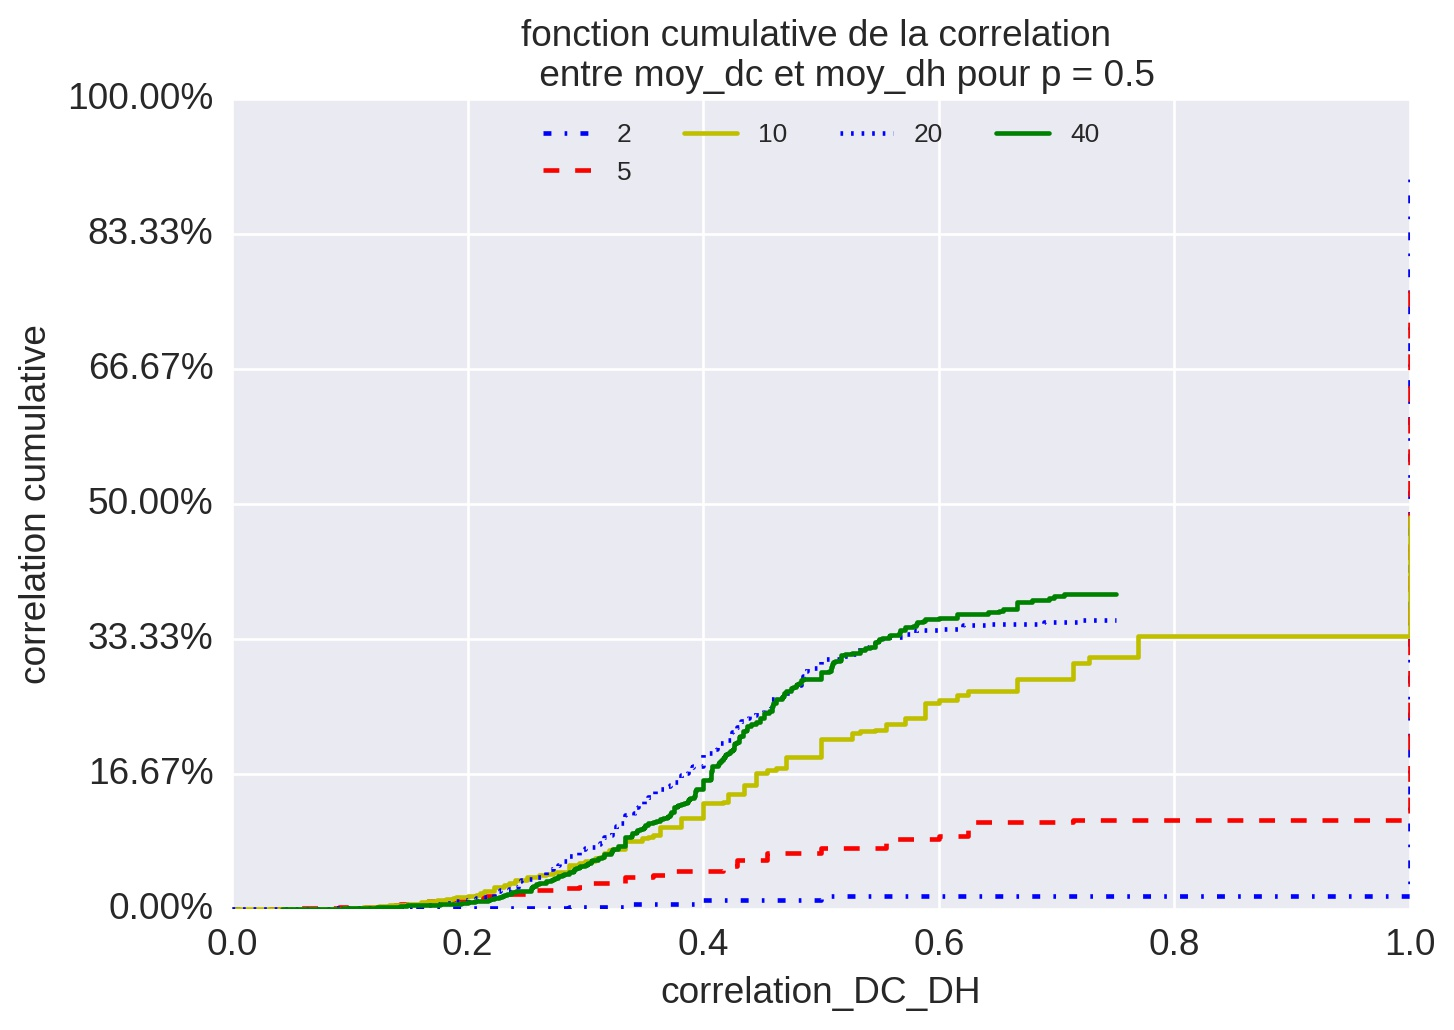
\includegraphics[scale=0.35]{correlation_dh_dl_p_05.jpeg}
\caption{ La corr\'elation de la distance de correction versus la distance de Hamming pour $k$ cases modifi\'ees et $p = 0.5$ }
\label{dh_vs_dc_p_05} 
\end{figure}
\FloatBarrier
% ----------------------------- figure  correlation distance hamming distance correlation -------------------- 

Nous calculons la corr\'elation entre les distances de correction et de Hamming avec la formule \ref{correlation_correction_hamming}.
%\begin{multline}
\begin{equation}
	corr_{k,p,\alpha} =  \frac{ | moy\_DC_{k, p,\alpha} - moy\_DH_{k,p, \alpha} | }{ max(moy\_DC_{k, p,\alpha},  moy\_DH_{k, p, \alpha}) };
	\\
	corr_{k,p} = \sum_{\alpha = 1}^{5}corr_{k,p,\alpha} ;
	\\ \newline
	F_k (x,p) = P(corr_{k,p} < x ) 
\label{correlation_correction_hamming}
\end{equation}
%\end{multline}
avec $x \in [0,1]$ une valeur de corr\'elation et $k$ le nombre de cases modifi\'ees. 
La fonction $corr_{k,p,\alpha}$ retourne l'\'ecart entre ces deux distances sous la forme de valeurs probabilistes. 
Ainsi $corr_{k,p,\alpha} = 1$ indique qu'il n'existe aucune corr\'elation entre les distances de correction et de Hamming c'est-\`a-dire que $moy\_DC_{k,p,\alpha} = k$ et $moy\_DH_{k,p,\alpha} = 0$.
De m\^eme, $corr_{k,p} = 0$ indique que ces distances sont identiques c'est-\`a-dire $ moy\_DC_{k, p, \alpha} = moy\_DH_{k,p, \alpha}$. En moyenne, $moy\_DH_{k,p, \alpha}$ tend vers $k$ cases modifi\'ees. 
\newline

La figure \ref{dh_vs_dc_p_05} repr\'esente la fonction de repartition $F_k$ dans laquelle nous avons, en abscisse, la corr\'elation entre les distances et, en ordonn\'e, le pourcentage de graphes dont la corr\'elation moyenne $corr_{k,p}$ est inf\'erieure \`a $x \in [0,1]$. 
%si $F_k$ a une courbe d'\'equation $y = 100$  ====> intuition pour la definition F_k
Si $corr_{k,p,\alpha} = 0$ alors les matrices de $LG_{k,p,\alpha}$ et $LG$ sont diff\'erentes de $k$ cases quand $k < 6$ ($LG_{k,p,\alpha} \neq LG$).
Si $corr_{k,p,\alpha} = 1$ alors le line-graphe $LG_{k, p, \alpha}$ est le line-graphe du graphe $G$ ($LG_{k, p, \alpha} = LG$) et $F_k(1) \approx 0$. 
La corr\'elation $corr_{k,p} = 1$ est sa valeur maximale. 
Ce cas est illustr\'e dans la figure \ref{dh_vs_dc_p_05} par les courbes de $k \in \{2,5\}$. 
Par exemple $F_5(1) \approx 10\%$ signifie que nous avons $70-10=60\%$ des line-graphes $LG_k$ qui ont le m\^eme ensemble d'ar\^etes que les line-graphes $LG$ ($70\%$ est le pourcentage de corr\'elations \'egales \`a $1$ $|corr_{5,p} = 1 | = 70\%$ ).
\newline
En revanche, une valeur de $F_k(1)$ tr\`es \'elev\'ee signifie que le nombre $x$ de  $corr_{k,p} = 1$ est tr\`es faible. Ce nombre $x$ implique une corr\'elation tr\`es forte entre les distances de correction et de Hamming.
C'est l'observation faite avec les courbes de $k \in \{10,20,40\}$ de la figure \ref{dh_vs_dc_p_05} dans lesquelles nous avons une  croissance continue en fonction de l'augmentation des valeurs de corr\'elations.
\newline
Nous subdivisons nos courbes en deux cat\'egories:
\begin{itemize}
	\item Celles pour lesquelles il y a une corr\'elation entre les distances de correction et de Hamming (courbes de $k \in \{10,20,40\}$).
	\item Celles pour lesquelles il y a  aucune corr\'elation entre ces distances parce que   $LG = LG_{k,p}$ (courbes de $k \in \{2,5\}$). 
\end{itemize}


{\bf Conclusion} :
il existe de fortes corr\'elations entre les distances de correction et de Hamming lorsque $k \ge 10$. Dans ce cas, nous pouvons utiliser la distance de correction pour calculer les \'ecarts de cases modifi\'ees pendant l'algorithme de correction.
Dans le cas o\`u $k \le 5$, les distances de correction inf\'erieures ou \'egales \`a $5$ cases proposent le line-graphe $LG$ et ces distance entrainent une corr\'elation proche de $0$.
Pour  $k \in \{6,7,8,9\}$, les valeurs de $corr_{k,p}$ avoisinent $0.5$. Ces valeurs sont faibles et nous ne pouvons rien conclure.
Ainsi, pour juger de la qualit\'e de notre algorithme de correction en l'absence de la distance de Hamming, la distance de correction est alors une bonne m\'etrique.

%		\subsubsection{Influence de la fonction de co\^ut sur les distributions de Hamming}
%			\label{influenceFonctionCoutDistributionHamming1}
%			\input{influenceFonctionCoutDistributionHamming1}
	\subsection{Conclusion de l'exp\'erimention 1}	
		
%----- conclusion 
Les performances de notre couple d'algorithmes ont \'et\'e test\'ees sur des graphes non orient\'es sans circuits qui repr\'esentent la topologie de r\'eseaux \'electriques. Nous avons construit les line-graphes de ces graphes et avons modifi\'e $k$ cases dans les matrices des line-graphes. Les cases modifi\'ees sont reparties en deux ensembles (cases {\em fausses positives} et {\em fausses n\'egatives}) selon la variable $p \in [0,1]$.
L'analyse des performances compare les distances de correction et de Hamming en fonction du nombre de cases modifi\'ees selon $5$ approches de correction et $3$ fonctions de co\^ut (voir tableau \ref{tab:recapApprocheCorrection}). 
Nous concluons que l'approche {\em al\'eatoire sans remise} donne de meilleurs r\'esultats lorsque le nombre $k$ de cases modifi\'ees est faible ($k\le 5$). La distance line est alors major\'ee par la distance de correction.  Le probl\`eme {\em Proxi-Line} a une solution mais elle n'est pas optimale.
En revanche, au-del\`a de $k > 5$, il est alors difficile de d\'eterminer une borne sup\'erieure \`a la distance line car l'algorithme de correction  modifie des cases n'\'etant pas contenues dans les $k$ cases modifi\'ees pr\'ealablement. 
Par ailleurs, nous avons montr\'e que la distance de correction peut \^etre utilis\'ee comme une m\'etrique pour connaitre le nombre de cases modifi\'ees dans la matrice d'un graphe \`a condition que cette distance soit sup\'erieure \`a $10$ ar\^etes. 
Enfin, les fonctions de co\^ut ont peu d'influence sur les distances de correction pendant la phase de correction.

%----- conclusion


%---------------------------------------------------------------------------
%------- 		experimentation 2 	---------------------
%---------------------------------------------------------------------------
\section{Exp\'erimentation 2 : Ajout de probabilit\'e dans la matrice du line-graphe}

Notre seconde exp\'erimentation a le m\^eme but que la premi\`ere sauf qu'ici la modification des cases est faite \`a partir de valeurs de seuils appliqu\'ees \`a des matrices de corr\'elation. Les valeurs de ces matrices sont d\'efinies selon la distribution des valeurs de corr\'elation d'un r\'eseau r\'eel, celui du datacenter {\em Champlan}.
\newline
Notre but est de d\'eterminer la valeur de seuil qui minimise les distances de correction et de Hamming obtenues avec l'approche {\em al\'eatoire sans remise} (tableau \ref{tab:recapApprocheCorrection}). 
\newline
Nous d\'ecrivons tout d'abord l'affectation des valeurs de corr\'elation aux cases de la matrice du line-graphe. Ensuite nous pr\'esentons les diff\'erentes \'etapes de notre exp\'erimentation et enfin nous analysons les r\'esultats obtenus.
	\subsection{Affectation de probabilit\'es aux cases de la matrice $M_{LG}$}
		\label{affectationValeursProbabilites}
		%---------------- distribution_0_1_metrique_wil_shapelets_P_len4950 ------------------
\begin{figure}[htb!] 
\centering
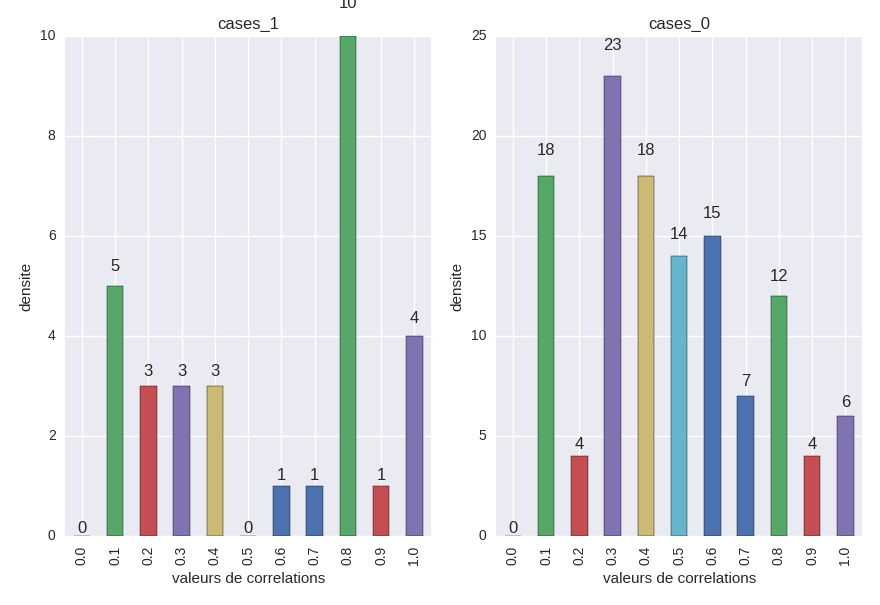
\includegraphics[width=500pt,height=250pt]{distribution_0_1_metrique_wil_shapelets_P_len4950.jpeg}
\caption{ Distribution des valeurs de corr\'elation de $M_c$ selon les cases \`a $0$ (\`a gauche) et \`a $1$ (\`a droite) de $M_{LG}$. La corr\'elation \`a $0.1$ d\'esigne  les valeurs de corr\'elation comprises entre $0.10$ et $0.199$. }
\label{distribution_0_1_metrique_wil_shapelets_P_len4950} 
\end{figure}
% \FloatBarrier
%---------------- distribution_0_1_metrique_wil_shapelets_P_len4950 ------------------


Soient la matrice $M_{LG}$ d'adjacence du line-graphe $LG$ du DAG non orient\'e de {\em Champlan} et $M_c$ sa matrice de corr\'elation obtenue avec la {\em distance de Pearson}.
 La distribution de valeurs de $M_c$ est repr\'esent\'ee par la figure \ref{distribution_0_1_metrique_wil_shapelets_P_len4950}. Le graphique \`a gauche de la figure \ref{distribution_0_1_metrique_wil_shapelets_P_len4950}  est la distribution des valeurs de $M_c$ selon les cases \`a $1$ dans $M_{LG}$ et le graphique \`a droite est celui des cases \`a $0$ dans $M_{LG}$. 
 Par exemple, la valeur de corr\'elation $0.1$ d\'esigne toutes les valeurs appartenant \`a $[0.1, 0.2[$. 
% En d'autres termes, ces distributions sont les celles des valeurs des cases {\em vrai n\'egatives} et {\em vrai positives}.
\newline
La densit\'e des  corr\'elations est d\'ecroissante pour les cases \`a $0$ quand les valeurs de corr\'elation tendent vers $1$. De m\^eme, cette densit\'e est croissante pour les cases \`a $1$ quand les corrections tendent vers $1$. La matrice $M_c$ contient des cases \'erron\'ees et ces cases ont une influence sur le calcul des valeurs de corr\'elation. C'est pourquoi les distributions ne sont pas lin\'eairement croissantes ou d\'ecroissantes.
Nous d\'ecidons, avec nos constatations, que la g\'en\'eration des distributions des valeurs de corr\'elation des cases \`a $0$ et $1$ suivent des lois normales asym\'etriques.
\newline

Nous  g\'en\'erons des valeurs de corr\'elation qui sont similaires \`a la distribution conjectur\'ee des valeurs de corr\'elation  du graphe de {\em Champlan}. Nous supposons que les valeurs de corr\'elation des cases \`a $0$ de $M_{LG}$ suivent la loi asym\'etrique de param\`etre $\alpha = 5$ et les valeurs de corr\'elation  des cases \`a $1$ de $M_{LG}$ suivent  cette m\^eme loi avec $\alpha = -5$ comme illustr\'e dans la figure \ref{distributionsCases01avecCoefficientAsymetries}. 
%---------------- distributionsCases01avecCoefficientAsymetries ------------------
\begin{figure}[htb!] 
\centering
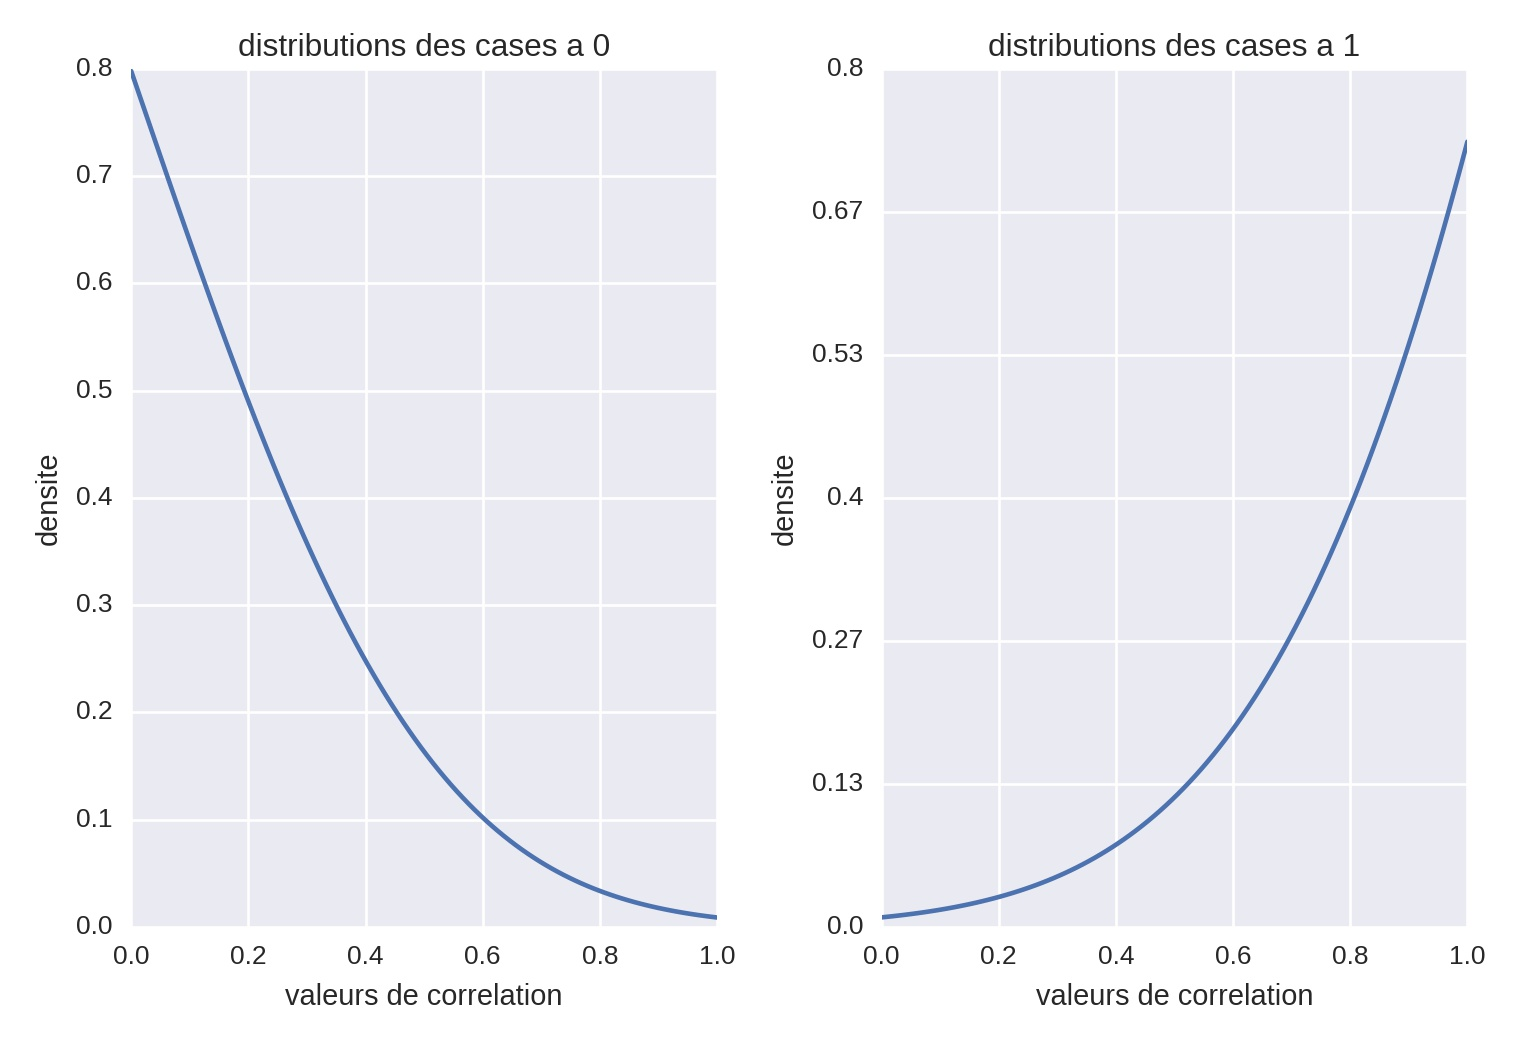
\includegraphics[width=500pt,height=250pt]{distributionsCases01avecCoefficientAsymetries.jpeg}
\caption{ Distribution des cases \`a $0$ et \`a $1$. \`A gauche : loi asym\'etrique de coefficient d'asym\'etrie $\alpha = 5$ pour les cases \`a $0$.  \`A droite : loi asym\'etrique de coefficient d'asym\'etrie $\alpha = -5$ pour les cases \`a $1$.}
\label{distributionsCases01avecCoefficientAsymetries} 
\end{figure}
% \FloatBarrier
%---------------- distributionsCases01avecCoefficientAsymetries ------------------
\newline

Soient 
$n_0$ la cardinalit\'e de l'ensemble des cases \`a $0$  de $M_{LG}$ et $n_1$ la cardinalit\'e de l'ensemble des cases \`a $1$ de $M_{LG}$.
Pour obtenir des valeurs de corr\'elation de $M_c$, nous g\'en\'erons  des valeurs r\'eelles $val$ appartenant \`a $[0,1]$ selon la loi asym\'etrique de coefficient $\alpha = 5$. Nous divisons l'intervalle $ [0,1]$ en $10$ sous-intervalles. Chaque sous-intervalle est not\'e  $]x_i,x_{i+1}]$ avec $x_i$ une valeur de corr\'elation et $i \in [0, 9]$. Nous calculons la densit\'e de chaque sous-intervalle et l'ensemble des densit\'es forme un histogramme qui suit une loi asym\'etrique.
Nous calculons la fonction de repartition $P$ de chaque densit\'e de telle sorte que 
$$
\forall x_i, x_{i+1}, P(X \le x_i) \le P(X \le x_{i+1}) ~~ et ~~ P(X \le x_{10}) = 1.
$$
\newline
Pour chaque case \`a $0$, nous tirons al\'eatoirement $n_0$ nombres r\'eels compris entre $0$ et $1$ uniformement. Si un nombre appartient \`a $]P(X \le x_i), P(X \le x_{i+1}) ]$ alors sa valeur de corr\'elation est $x_{i+1}$. Nous r\'ep\'etons les m\^emes \'etapes pour les cases \`a $1$ en g\'en\'erant les valeurs $val$ avec une loi asym\'etrique de coefficient $\alpha = -5$.
Nous obtenons la matrice de corr\'elation $M_c$ du line-graphe $LG$. Une distribution des valeurs de corr\'elation est repr\'esent\'ee par la figure \ref{distribution01} dans laquelle nous avons $189$ cases \`a $0$ et $111$ cases \`a $1$ dans $LG$.
%---------------- distribution01 ------------------
\begin{figure}[htb!] 
\centering
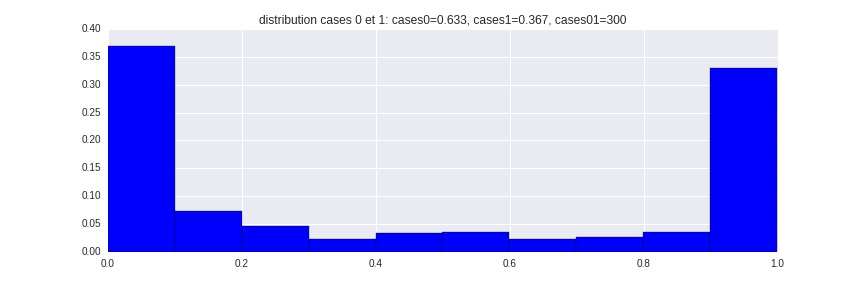
\includegraphics[width=550pt,height=250pt]{distribution01.jpeg}
\caption{ Un exemple de la distribution des valeurs de corr\'elations g\'en\'er\'ees. $63\%$ des cases sont des cases \`a 0 et $37\%$ sont des cases \`a $1$ dans $LG$.}
\label{distribution01} 
\end{figure}
% \FloatBarrier
%---------------- distribution01 ------------------


	\subsection{G\'en\'eration du graphe de corr\'elation }
		\label{experimentation2GenerationMatriceProbabiliteAvecSeuil}
		Nous allons d\'eterminer la matrice d'adjacence du graphe de corr\'elation \`a partir des valeurs de $M_c$.
\newline 
Soit $s = \{ 0.1, \cdots, 0.9\}$, une valeur de seuil choisie.
Nous construisons la matrice $M_s$  selon les r\`egles suivantes : 
\begin{itemize}
\item Si $M_c[i,j] \ge s$ alors $M_s[i,j] = 1$.
\item Si $M_c[i,j] < s$ alors $M_s[i,j] = 0$.
\end{itemize}
La matrice $M_s$ est la matrice d'adjacence du graphe $G_s$  dit {\em graphe de corr\'elation}. Ces cases peuvent contenir des cases erron\'ees. Ces cases erron\'ees proviennent de la s\'election du seuil $s$ et de la g\'en\'eration de valeurs de corr\'elation pour les cases \`a $0$ et \`a $1$ du line-graphe $LG$. En effet ,
\begin{itemize}
	\item Si $M_s [i,j] = M_{LG} [i,j] = 0$ alors $M_{s} [i,j]$ est dit {\em vrai n\'egatif}. 
	\item Si $M_s [i,j] = M_{LG} [i,j] = 1$ alors $M_{s} [i,j]$ est dit {\em vrai positif}. 
	\item Si $M_s [i,j] = 0$ et $M_{LG} [i,j] = 1$ alors $M_{s} [i,j]$ est dit {\em faux n\'egatif}.
	\item Si $M_s [i,j] = 1$ et $M_{LG} [i,j] = 0$ alors $M_{s} [i,j]$ est dit {\em faux positif}.
\end{itemize}
Un exemple de distributions des cases erron\'ees selon les valeurs de seuils est pr\'esent\'e dans la figure \ref{distrib_relationAdjacence_seuils}. 
%---------------- distributionsCases01avecCoefficientAsymetries ------------------
\begin{figure}[htb!] 
\centering
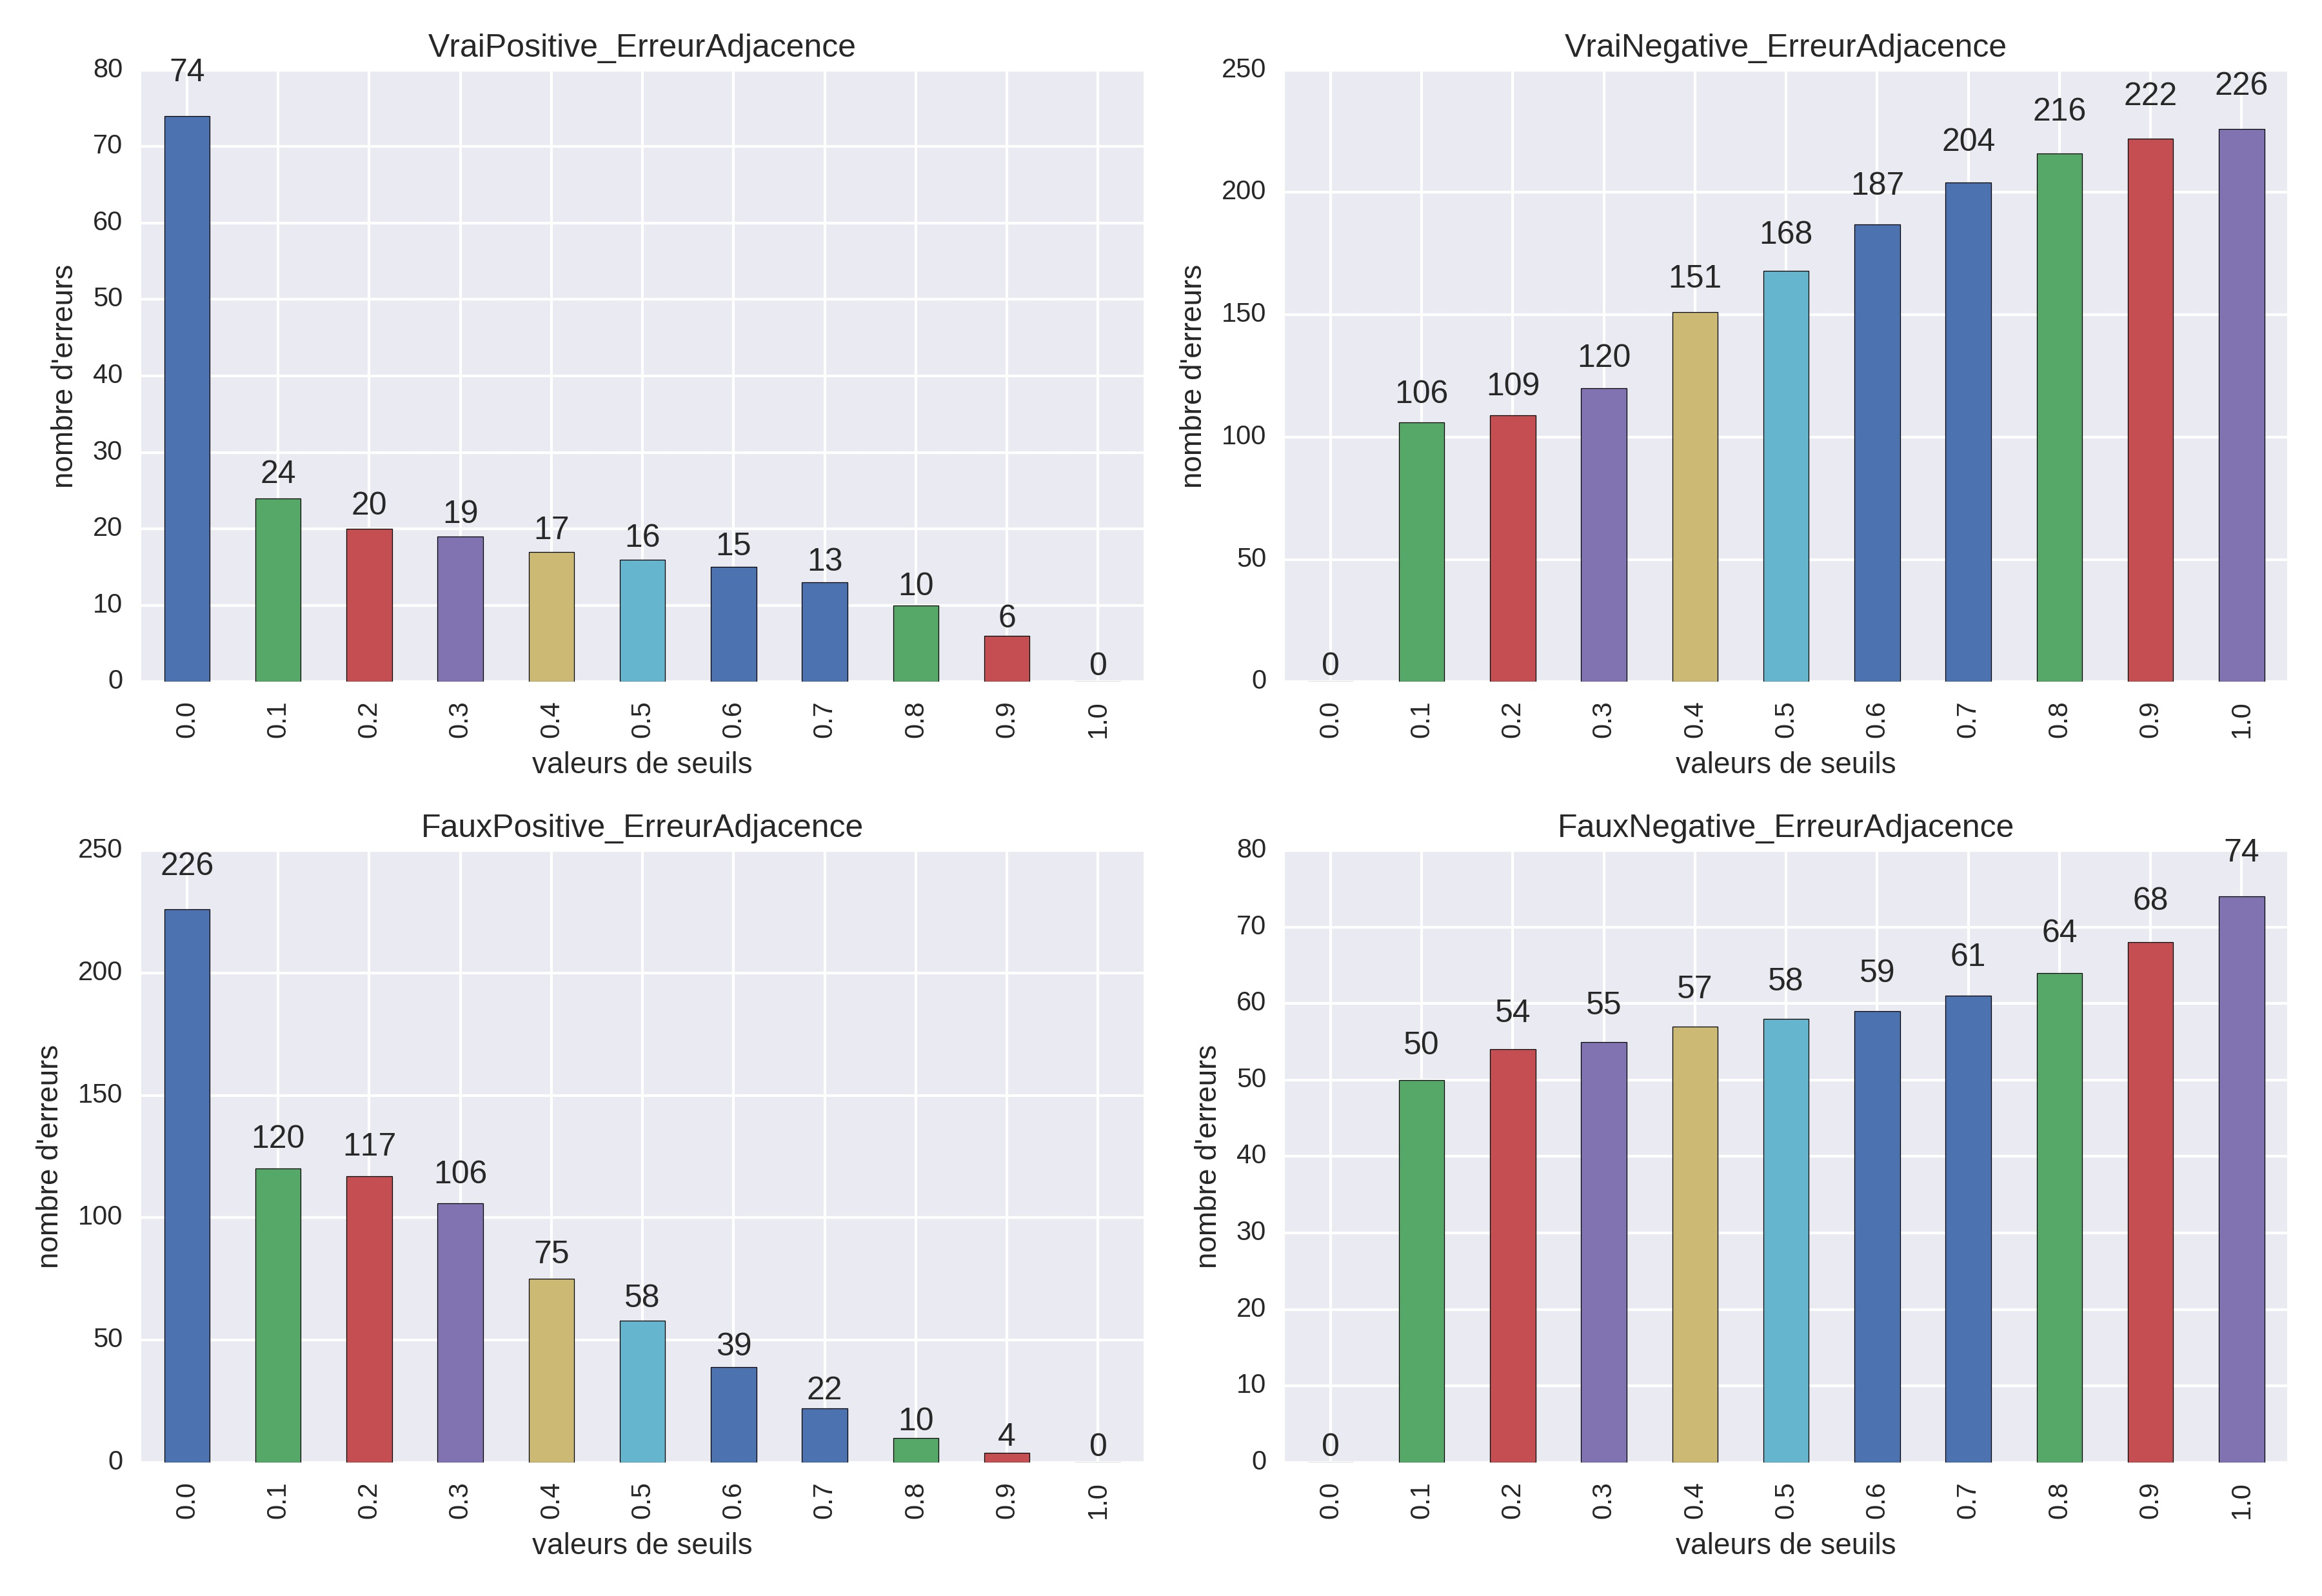
\includegraphics[width=500pt,height=250pt]{distrib_relationAdjacence_seuils.jpeg}
\caption{ Distribution des valeurs de corr\'elation sur un graphe g\'en\'er\'e de $30$ sommets et de degr\'e maximal de $5$.
.}
\label{distrib_relationAdjacence_seuils} 
\end{figure}
% \FloatBarrier
%---------------- distributionsCases01avecCoefficientAsymetries ------------------
Par exemple,  le graphe de corr\'elation $G_s$ contient 
$17$ cases {\em vrais positives}, 
$151$ cases {\em vrais n\'egatives}, 
$75$ cases {\em fausses positives} et 
$57$ cases {\em fausses n\'egatives} pour un seuil $s=0.4$.

	\subsection{Protocole d'exp\'erimentation des graphes  $G_s$ de corr\'elation} 
		% ------------- recapProtocoleEtudeSeuil -------------
\begin{figure}[htb!] 
\centering
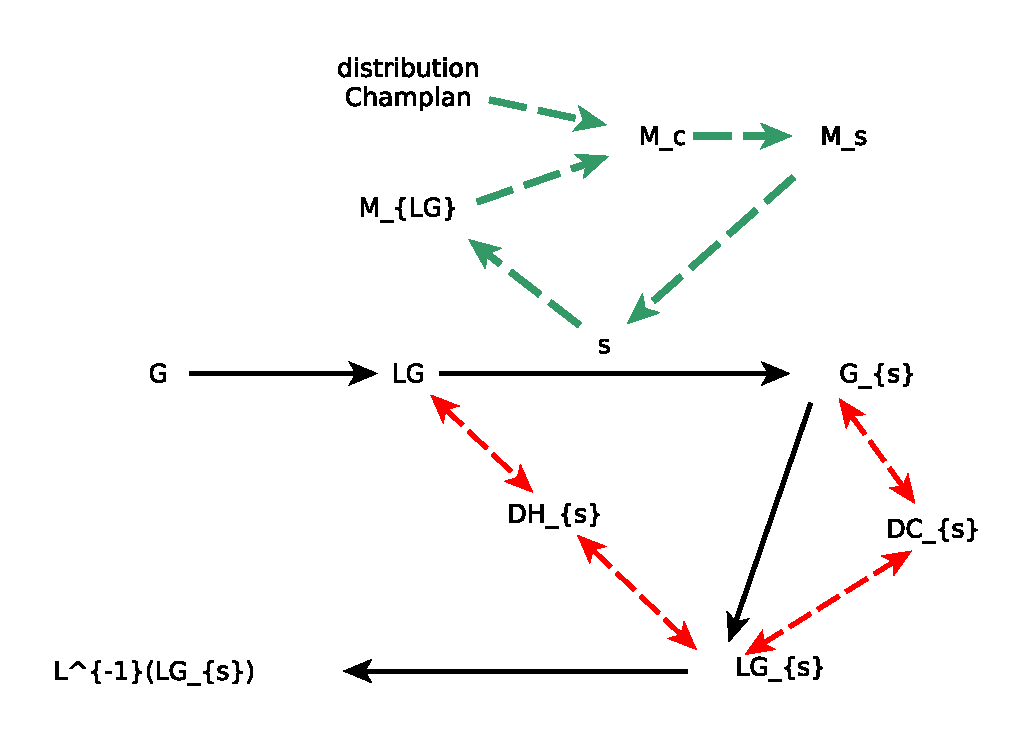
\includegraphics[scale=0.750]{recapProtocoleEtudeSeuil.eps}
\caption{\'Etapes de l'exp\'erimentation :  
1) on g\'en\`ere le graphe $G$ et son line-graphe $LG$, 
2) on  g\'en\`ere la matrice de corr\'elation $M_c$ du line-graphe $LG$   \`a partir de la distribution des valeurs de corr\'elation du graphe de Champlan puis on lui applique une valeur de seuil $s$ pour obtenir le graphe $G_{s}$, 
3) on applique les algorithmes de d\'ecouverte et de correction pour avoir un line-graphe $LG_{s}$. $LG_{s}$ et  $G_{s}$ diff\`erent de $DC_{s}$ ar\^etes. $LG_{s}$ a $DH_{s}$ cases modifi\'ees par rapport \`a $LG$, 
4) $L^{-1}(LG_{s})$ est le graphe racine de $LG_{s}$. 
}
\label{recapProtocoleEtudeSeuil} 
\end{figure}
% FloatBarrier
% ------------- recapProtocoleEtudeSeuil -------------

Le but de notre couple d'algorithmes est de corriger les cases erron\'ees dans $M_s$ afin que la matrice propos\'ee $M'_{s}$ soit la matrice d'adjacence d'un line-graphe $LG_s$ et que la distance de Hamming entre $LG_s$ et $LG$ soit minimale. 
Pour ce faire, nous recherchons la valeur du seuil $s$ qui mininise la distance de Hamming entre $LG_s$ et $LG$.
\newline

Nous g\'en\'erons les graphes dans les m\^emes conditions que l'exp\'erimentation $1$ de la section \ref{experimentation1} avec de petites modifications. D'abord, le nombre de graphes g\'en\'er\'es est de $150$. Ensuite, nous construisons une matrice de corr\'elation dont les \'etapes sont d\'ecrites dans la section \ref{affectationValeursProbabilites}. Et enfin, l'ajout des cases erron\'ees est r\'ealis\'e \`a partir d'un seuil $s$ dans la matrice de corr\'elation $M_c$ comme cela est expliqu\'e dans la section \ref{experimentation2GenerationMatriceProbabiliteAvecSeuil}. 
Les \'etapes de l'exp\'erimentation sont r\'esum\'ees dans la figure \ref{recapProtocoleEtudeSeuil}.

Nous consid\'erons que l'approche {\em al\'eatoire sans remise} (tableau \ref{tab:recapApprocheCorrection}) pendant l'algorithme de correction. Mais les fonctions de co\^uts des ar\^etes utilisent les valeurs de corr\'elation comme suit:
\begin{enumerate} [label = (\alph*)]
\item {\em Unitaire} : l'ajout et la suppression d'une ar\^ete ont un co\^ut de $1$.
\item {\em Normale} : l'ajout d'une ar\^ete \`a la case $M_s[i,j]$ a un co\^ut \'egal \`a sa valeur de corr\'elation $M_c[i,j]$ et la suppression d'une ar\^ete a un  co\^ut $1-M_c[i,j]$.
\item {\em Ajout} : l'ajout d'une ar\^ete \`a la case $M_s[i,j]$ a un co\^ut $M_c[i,j]$ alors que la suppression \`a cette case a un co\^ut $2 \times (1-M_c[i,j])$.
\item {\em Suppression} : la suppression d'une ar\^ete \`a la case $M_s[i,j]$ a un co\^ut $1-M_c[i,j]$ alors que l'ajout d'une ar\^ete \`a cette case a un co\^ut $2 \times M_c[i,j]$.
\end{enumerate}
Nous allons comparer les distances de Hamming et le pourcentage de cases corrig\'ees pour en d\'eduire la bonne valeur de seuil.



	\subsection{Analyses des r\'esultats}
	Nous allons d\'ecrire l'\'evolution du pourcentage des cases corrig\'ees en fonction de la valeur du seuil pour la fonction de co\^ut {\em normale}. Ensuite nous d\'eterminons l'influence de la valeur de seuil sur le nombre de cases corrig\'ees et enfin nous recherchons la meilleure fonction de co\^ut et l'influence des fonctions de co\^ut sur l'\'evolution des distances de Hamming.
		\subsubsection{\'Evolution du pourcentage de cases corrig\'ees}
			
Pour mesurer le pourcentage de cases corrig\'es, nous allons proc\'eder comme suit :
\begin{enumerate}[label = (\alph*)]
	\item Consid\'erer les cases {\em fausses positives} dans la matrice $M_s$ puis repr\'esenter le nombre de cases {\em fausses positives} pour chaque valeur de seuil. 
	Le graphique $(a)$ de la figure \ref{graphiquesFctCoutNormale} correspond \`a  la comparaison des seuils par rapport au nombre de cases {\em fausses positives} avant la correction.
	Nous remarquons qu'il n'y a aucune case {\em fausse positive} dans $M_s$ pour $s\in\{0.8,0.9\}$. Ce nombre croit quand le seuil $s$ decroit ($s \rightarrow 0$).
	
	\item Consid\'erer les cases {\em fausses n\'egatives} dans la matrice $M_s$ puis repr\'esenter le nombre de cases {\em fausses n\'egatives} pour chaque valeur de seuil.  Le graphique $(b)$ de la figure \ref{graphiquesFctCoutNormale}  correspond \`a la comparaison des seuils par rapport au nombre de cases {\em fausses n\'egatives} avant la correction. Le nombre des cases {\em fausses n\'egatives} est nul pour $s \not \in \{0.8,0.9\}$. 

	\item Consid\'erer les cases {\em fausses positives} apr\`es la correction de $G_s$ (matrice $M'_s$) puis repr\'esenter le nombre de cases {\em fausses positives} pour chaque valeur de seuil. Le graphique $(c)$ de la figure \ref{graphiquesFctCoutNormale} correspond \`a  la comparaison des seuils par rapport au nombre de cases {\em fausses positives} apr\`es la correction.
	 Le nombre de cases baisse quand $s \le 0.7$ puis augmente $s>0.7$.
	 
	\item Consid\'erer les cases {\em fausses n\'egatives} apr\`es la correction de $G_s$ (matrice $M'_s$) puis repr\'esenter le nombre de cases {\em fausses n\'egatives} pour chaque valeur de seuil. Le graphique $(d)$ de la figure \ref{graphiquesFctCoutNormale} correspond \`a la comparaison des seuils par rapport au nombre de cases {\em fausses n\'egatives} apr\`es la correction. Le nombre de cases varie peu quand $s < 0.4$ puis baisse quand $s = \{0.5, 0.6\}$ avant d'atteindre sa valeur minimum \`a $s = 0.7$. Il augmente $s>0.7$.
	
	\item Repr\'esenter les distances de Hamming moyennes de chaque graphe pour chaque seuil. Le graphique $(e)$ de la figure \ref{graphiquesFctCoutNormale} correspond \`a la comparaison des seuils en fonction de la distance de Hamming de chaque seuil.
	La distance de Hamming baisse quand $s \rightarrow 0.7$ avec sa valeur minimum \`a $s = 0.7$ puis augmente quand $s > 0.7$. 
\end{enumerate}
Rappelons que les diff\'erents graphiques sont rang\'es par ordre croissant et 
les distances de Hamming sont obtenues \`a partir la fonction de co\^ut {\em normale}.

Nous distinguons trois familles de seuils:
\begin{itemize}
	\item Les seuils $s < 0.7$ qui baissent le nombre de cases  {\em fausses positives} et augmentent celui des cases {\em fausses n\'egatives} apr\`es l'algorithme de correction. 
	Ils n'ont pas d'effets r\'eels sur la distance de Hamming car il y a un transfert d'\'el\'ements de l'ensemble des cases   {\em fausses positives} \`a celui des {\em fausses n\'egatives} et vice-versa. 
	\`A cet effet, on remarque  qu'il y a $20\%$ de cases {\em fausses n\'egatives} apr\`es la correction alors qu'il n'en existait aucune case {\em fausse n\'egative} avant la correction. 
	Il en est de m\^eme avec les cases  {\em fausses positives}  dont le nombre diminue de $20\%$  \'egalement pendant la correction. Ces seuils n'ont aucune influence sur les cases erron\'ees.
	% -------- graphiquesFctCoutNormale ---------
\begin{figure}[htb!] 
\centering
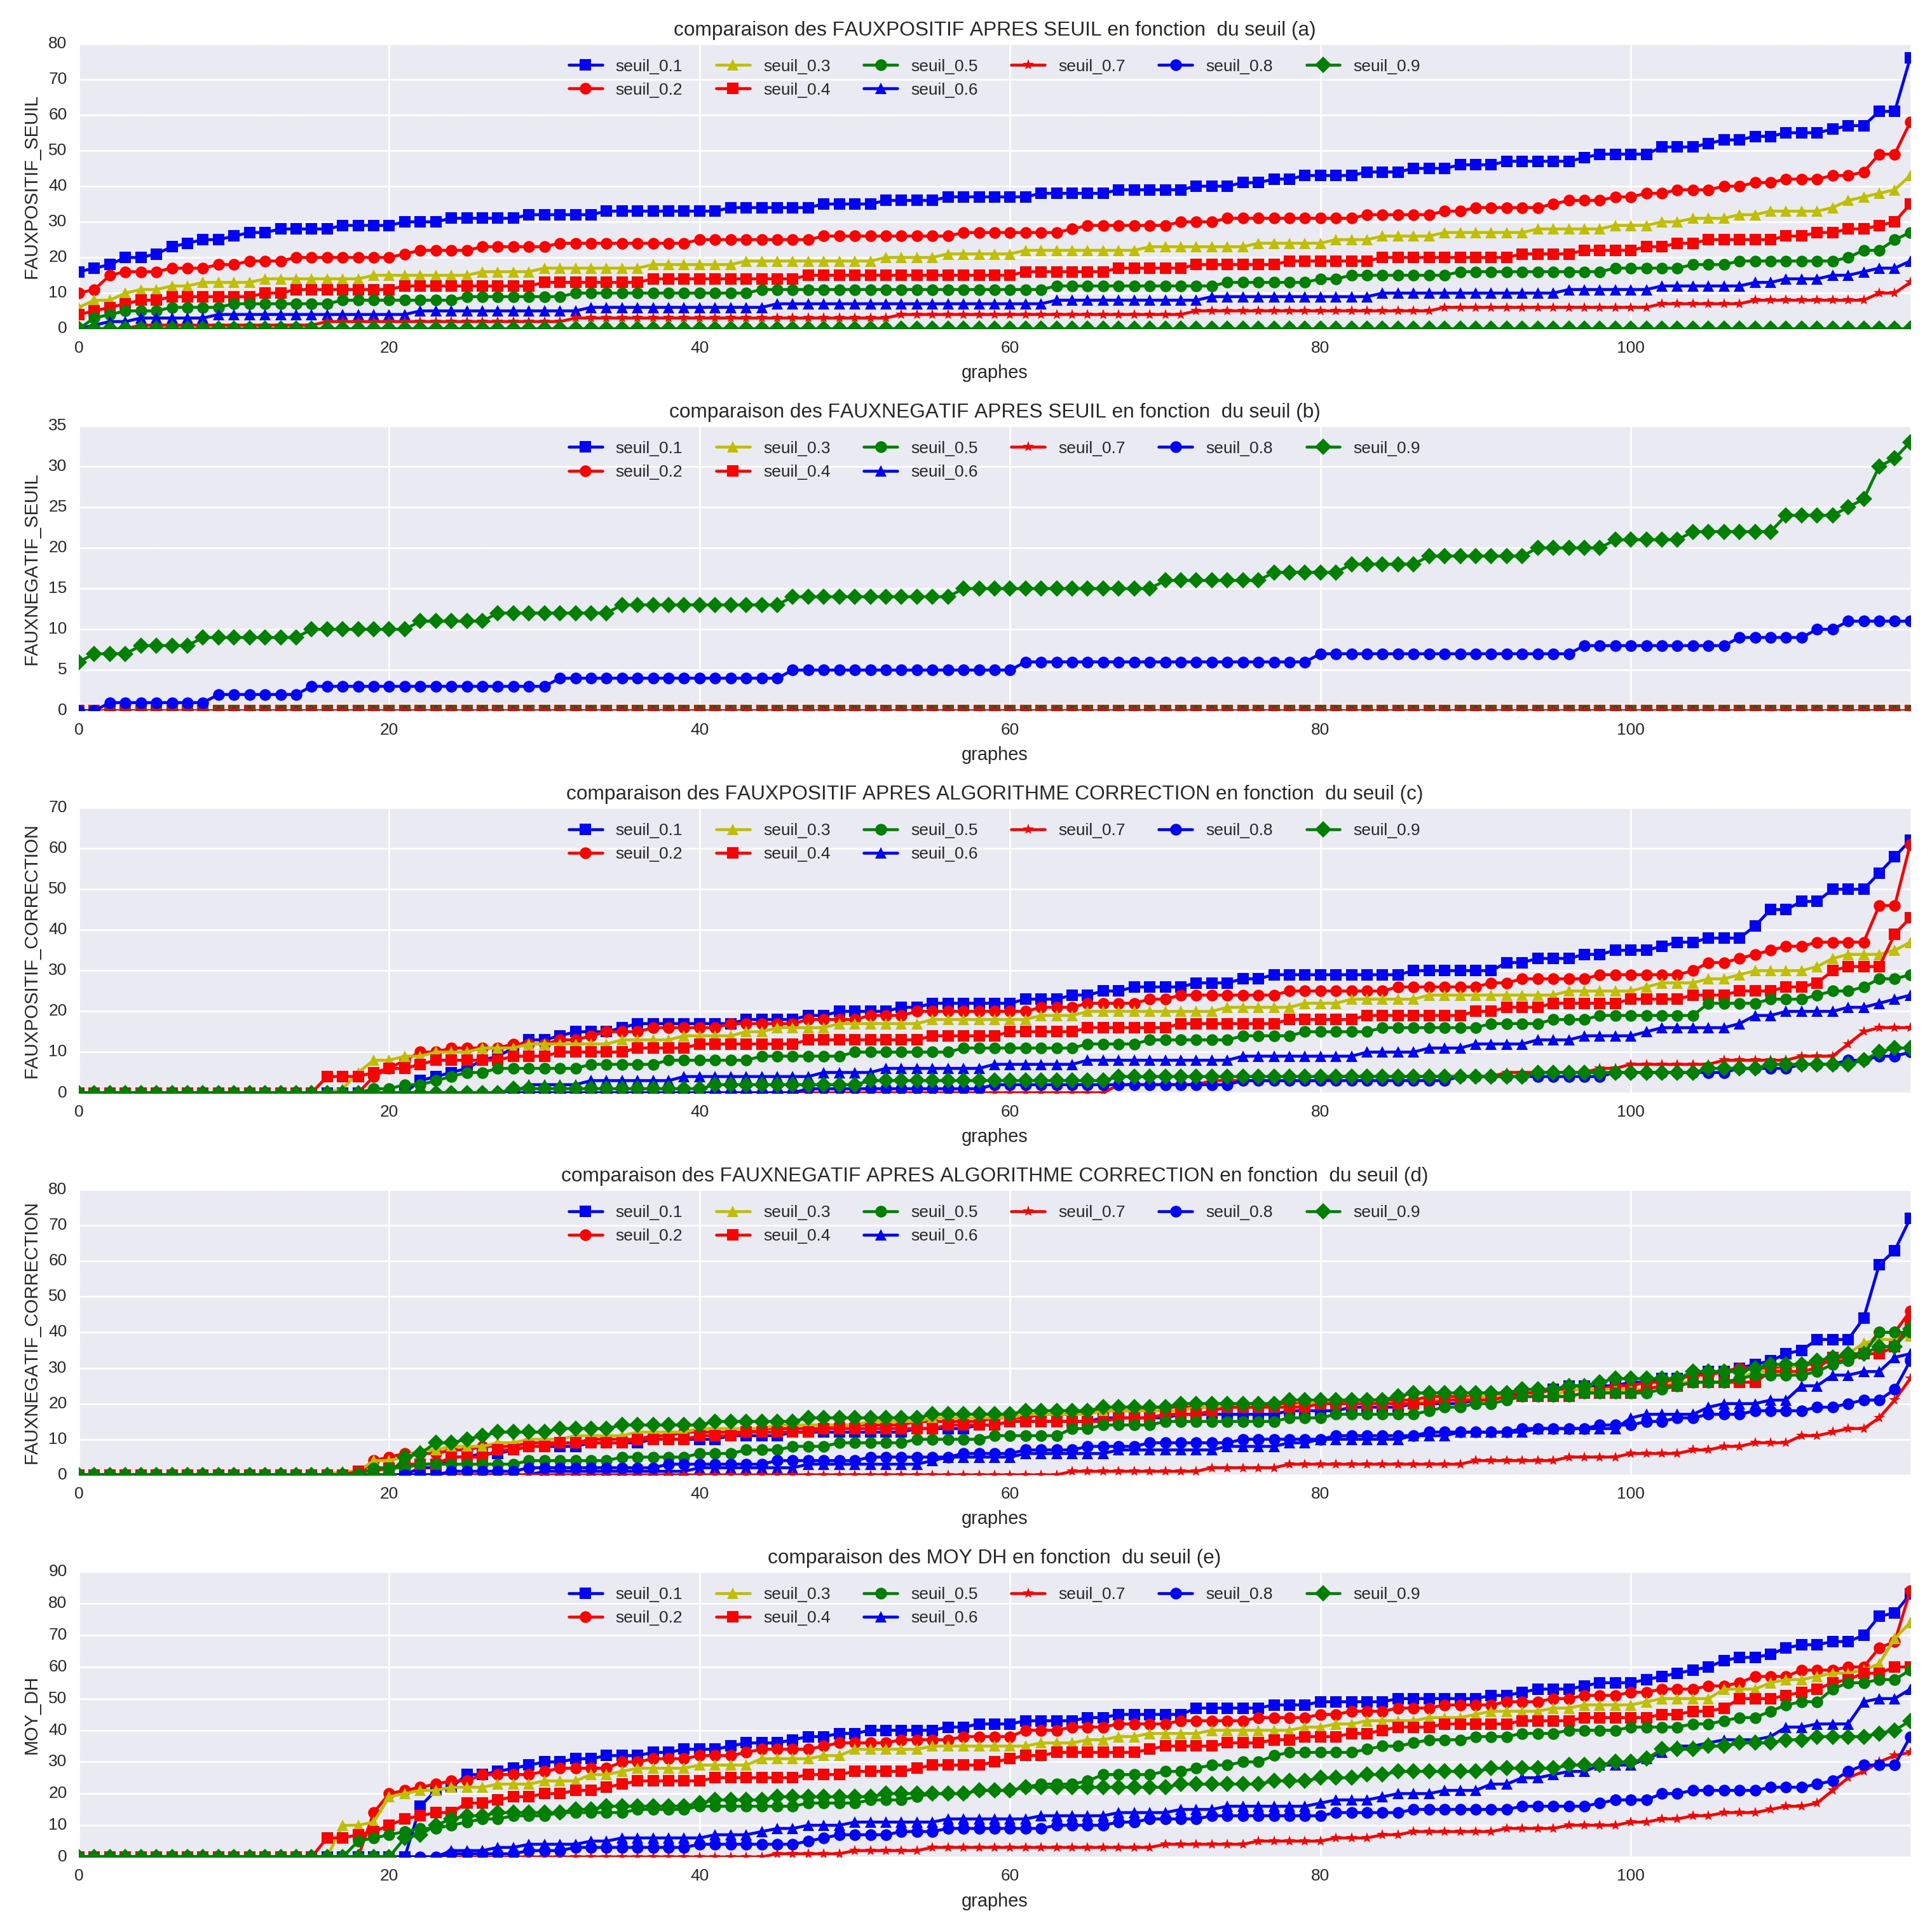
\includegraphics[scale=0.18]{choix_du_seuil_pour_fauxPositif_seuil_fauxNegatif_seuil_fauxPositif_correction_fauxNegatif_correction_moy_dh_aleatoire_normale.jpeg}
\caption{ Choix du seuil : (a) cases {\em fausses positives} dans la matrice $M_s$; (b) cases {\em fausses n\'egatives} dans la matrice $M_s$,(c) cases {\em fausses positives} dans la matrice $M'_s$; (d) cases {\em fausses n\'egatives} dans la matrice $M'_s$; (e) comparaison des seuils selon $moy\_DH$ }.
\label{graphiquesFctCoutNormale} 
\end{figure}
\FloatBarrier
% -------- graphiquesFctCoutNormale ---------

	\item Les seuils $s > 0.7$ qui augmentent le nombre de cases {\em fausses positives} et baissent celui des cases {\em fausses n\'egatives} apr\`es l'algorithme de correction. En effet, 
	le nombre de cases {\em fausses positives} est nul dans $M_s$ parce qu'il n'y a aucune case \`a $1$ ayant une valeur inf\'erieure \`a $s$ dans la distribution.
	Dans $M'_s$, le nombre moyen de cases {\em fausses positives} est de $1.76$ pour $s=0.8$ et de $2.33$ pour $s=0.9$. 
	Il y a l'ajout d'ar\^etes dans le graphe $LG_s$ parce que le nombre d'ar\^etes \`a supprimer pour corriger un sommet est tr\`es \'elev\'e et cela implique que le co\^ut de la correction par la suppression d'ar\^etes est tr\`es on\'ereux par rapport \`a celui de l'ajout d'ar\^etes. 
	Ainsi \`a chaque sommet \`a corriger, l'algorithme ajoute plus d'ar\^etes qu'il en supprime et certaines ar\^etes ajout\'ees appartiennent \`a l'ensemble des ar\^etes de $LG$.
	 Cela fait baisser les cases {\em fausses n\'egatives} comme nous le constatons avec les chiffres suivants : le nombre moyen de ces cases passe de  $6.7$ \`a $2.5$  pour $s = 0.8$ et de $17.7$ \`a $12.5$ pour $s = 0.9$.
	
	\item Le seuil $s=0.7$ qui diminue le nombre de cases {\em fausses n\'egatives} et {\em fausses positives}. En effet, le nombre moyen de cases erron\'ees est faible $< 10$ avant la phase de correction et il est $ \le 5$ apr\`es la correction. 
	Nous remarquons aussi les cases erron\'ees sont majoritairement des cases {\em fausses n\'egatives} apr\`es la correction.
	La pr\'esence de ces cases provient du co\^ut de modification des ar\^etes car la compression $\pi_1,\pi_2, \pi_s$ de co\^ut minimale n\'ecessite la suppression d'ar\^etes existantes.
	En effet, la matrice $M_s$ ne contient que des cases {\em fausses positives}. Pour trouver des bipartitions coh\'erentes (voir d\'efintion \ref{cliquesCoherentes}) autour des sommets \`a corriger, il faut ajouter beaucoup d'ar\^etes pour chaque partition et cela fait croitre le co\^ut de la correction. 
	Nous avons remarqu\'e aussi que la suppression de quelques ar\^etes permet d'obtenir des cliques qui correspondent \`a des sommets de $G$. L'algorithme pr\'ef\`ere alors supprimer des ar\^etes car elles sont peu par rapport aux ar\^etes \`a ajouter et aussi le co\^ut de la suppression d'ar\^etes est faible.
	 La distance de Hamming obtenue avec ce seuil est minimale par rapport aux autres seuils. Ce seuil fournit alors une meilleure correction des sommets de ${\cal C}$. 
	
\end{itemize}

{\bf Conclusion} : 
nous pouvons conclure que la repartition des cases erron\'ees avant la phase de correction a une influence sur l'algorithme de correction. 
Ainsi, le choix du seuil dans le bon intervalle permet de r\'eduire le nombre de cases erron\'ees et fournit une excellente correction des sommets de ${\cal C}$. 
Cependant,  les seuils diff\'erents du bon seuil  entraine que la fonction de co\^ut n'a aucune influence sur les corrections parce que l'algorithme corrige peu de cases erron\'ees mais ajoute aussi des cases {\em fausses positives} et {\em fausses n\'egatives} dans la m\^eme proportion. 

% ----------- comparaisonFctCoutUnitaireNormale -----------------
\begin{figure}[htb!] 
\centering
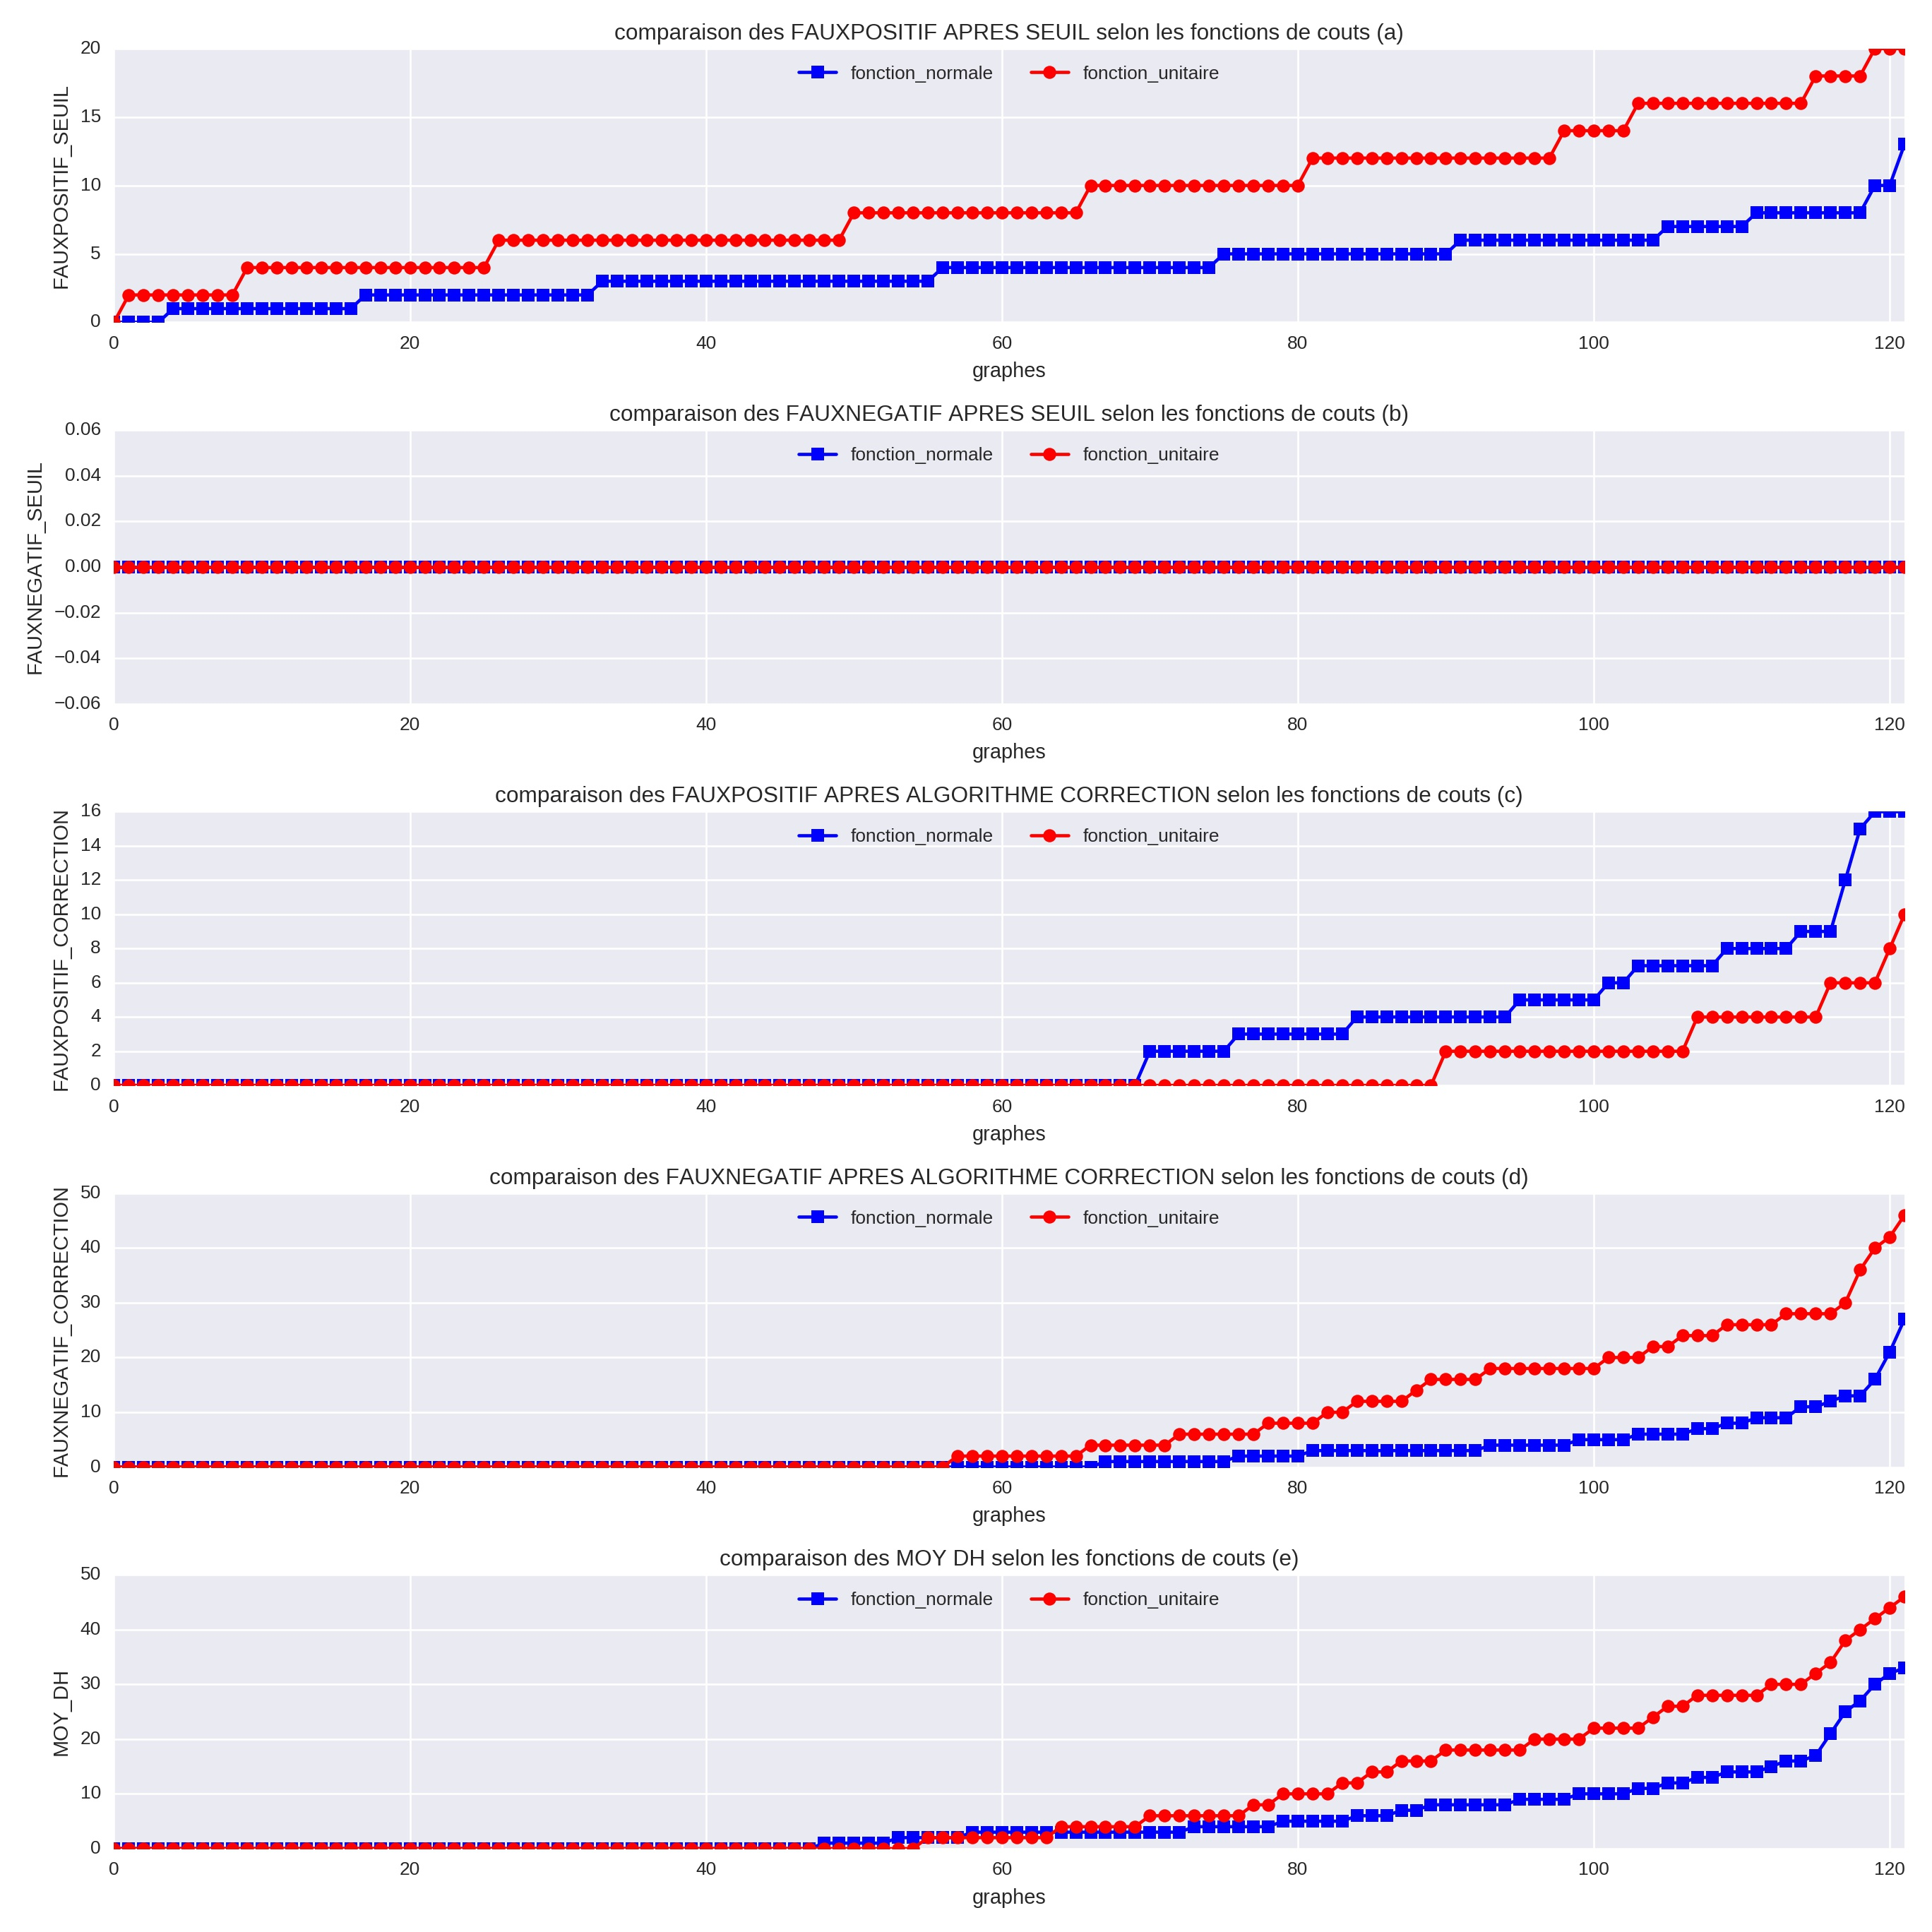
\includegraphics[scale=0.20]{choix_fct_cout_pour_fauxPositif_seuil_fauxNegatif_seuil_fauxPositif_correction_fauxNegatif_correction_moy_dh_aleatoire_s_07.jpeg}
\caption{ Comparaison entre les fonctions de co\^ut {\em unitaire} et {\em normale}: (a) cases {\em fausses positives} dans la matrice $M_s$; (b) cases {\em fausses n\'egatives} dans la matrice $M_s$; (c) cases {\em fausses positives} dans la matrice $M'_s$; (d) cases {\em fausses n\'egatives} dans la matrice $M'_s$; (e) comparaison des fonctions de co\^ut selon $moy\_DH$.}
\label{comparaisonFctCoutUnitaireNormale} 
\end{figure}
 \FloatBarrier
% ----------- comparaisonFctCoutUnitaireNormale -----------------


		\subsubsection{Influence de la valeur du seuil }
			%choix du seuil
Les seuils inf\'erieurs \`a $0.7$ correspondent \`a une reduction des cases {\em fausses positives} et une augmentation de cases {\em fausses n\'egatives} dans la matrice de correction. Dans ce cas, nous constatons que le nombre des  cases
{\em fausses positives} baisse \'enormement quand $s \rightarrow 0.7$. Ce ph\'enom\`ene s'explique par le co\^ut de modifications des ar\^etes (normale) et le nombre faible de cases erron\'ees au voisinage de  $0.7$. L'augmentation des cases  {\em fausses n\'egatives} provient du  fonctionnement de notre algorithme de correction.  L'algorithme doit ajouter des ar\^etes dans une partition $\pi_1 ~ou~ \pi_2$ au voisinage d'un sommet pour en faire une clique. Le nombre \'elev\'e de cases  {\em fausses n\'egatives} n\'ecessite l'ajout de beaucoup d'ar\^etes.
\newline
Les seuils sup\'erieurs \`a $0.7$ correspondent \`a l'augmentation des  cases {\em fausses positives} et la baisse de celles {\em fausses n\'egatives}. 
La pr\'esence de cases {\em fausses positives} en grand nombre entraine l'algorithme de correction dans deux cas :
l'ajout de peu d'ar\^etes  et 
la suppression de beaucoup d'ar\^etes pour atteindre un line-graphe.
Dans le premier cas, la distance de Hamming est faible mais le line-graphe est diff\'erent du line-graphe de $G_s$. 
Dans ce second cas, la distance de Hamming est tr\`es \'elev\'ee et nous avons tr\`es peu de chance de retrouver le line-graphe de $G_s$.
\newline

{\bf Conclusion} : 
le meilleur compromis de seuil est celui qui baisse les cases {\em fausses positives}  et les cases {\em fausses n\'egatives} apr\`es l'algorithme de correction.  Le seuil capable d'atteindre ce r\'esultat est dans l'intervalle $s=]0.6,0.7]$. Dans la suite du chapitre, nous retenons $s=0.7$.
Avec ce seuil, les distances de Hamming sont aussi les plus faibles (graphique $(e)$ figure \ref{graphiquesFctCoutNormale}). 
		\subsubsection{Choix de la fonction de co\^ut et impact sur les distances de Hamming }
			
Nous rappelons que la fonction de co\^ut est d\'efinie par la somme des co\^uts des cases \`a modifier pour corriger chaque sommet de $\cal C$ pendant l'algorithme de correction. 
Le co\^ut de correction d'un sommet est le co\^ut minimal de toutes les cases modifi\'ees. 
Nous recherchons alors la fonction de co\^ut qui minimise globalement le co\^ut de correction des sommets de $\cal C$.
%Pour ce faire, nous comparons les fonctions de co\^ut {\em unitaire}, {\em normale}, {\em ajout} et {\em suppression}. 
Pour ce faire, nous comparons d'abord les fonctions de co\^ut {\em unitaire} et {\em normale} parce que nous souhaitons savoir s'il est pr\'ef\'erable d'utiliser les valeurs de corr\'elations dans les co\^uts des op\'erations. Puis nous comparons la meilleure des deux fonctions avec celles {\em ajout} et {\em suppression}.
%Nous repr\'esentons les distances $moy\_DH$ des diff\'erentes fonctions de co\^ut  sur la figure \ref{comparaisonFctCoutUnitaireNormale}. 
La figure \ref{comparaisonFctCoutUnitaireNormale} contient 
\begin{itemize}
	\item La comparaison des distances de Hamming entre les  fonctions de co\^ut {\em unitaire} et {\em normale} (graphique $(e)$).
	\item La comparaison du nombre de cases {\em fausses n\'egatives} entre les $2$ fonctions de co\^ut avant l'algorithme de correction (graphique $(b)$).
	\item  La comparaison du nombre de cases {\em fausses n\'egatives} entre les $2$ fonctions de co\^ut apr\`es l'algorithme de correction (graphique $(d)$).
	\item La comparaison du nombre de cases {\em fausses positives} entre les $2$ fonctions de co\^ut avant l'algorithme de correction (graphique $(a)$).
	\item  La comparaison du nombre de cases {\em fausses positives} entre les $2$ fonctions de co\^ut apr\`es l'algorithme de correction (graphique $(a)$).
\end{itemize}
Les distances de Hamming et les nombres de cases sont ordonn\'ees par ordre croissant.
%\newline
% ----------- comparaisonFctCoutNormaleAjoutSuppression -----------------
\vspace{-0.5cm}
\begin{figure}[htb!] 
\centering
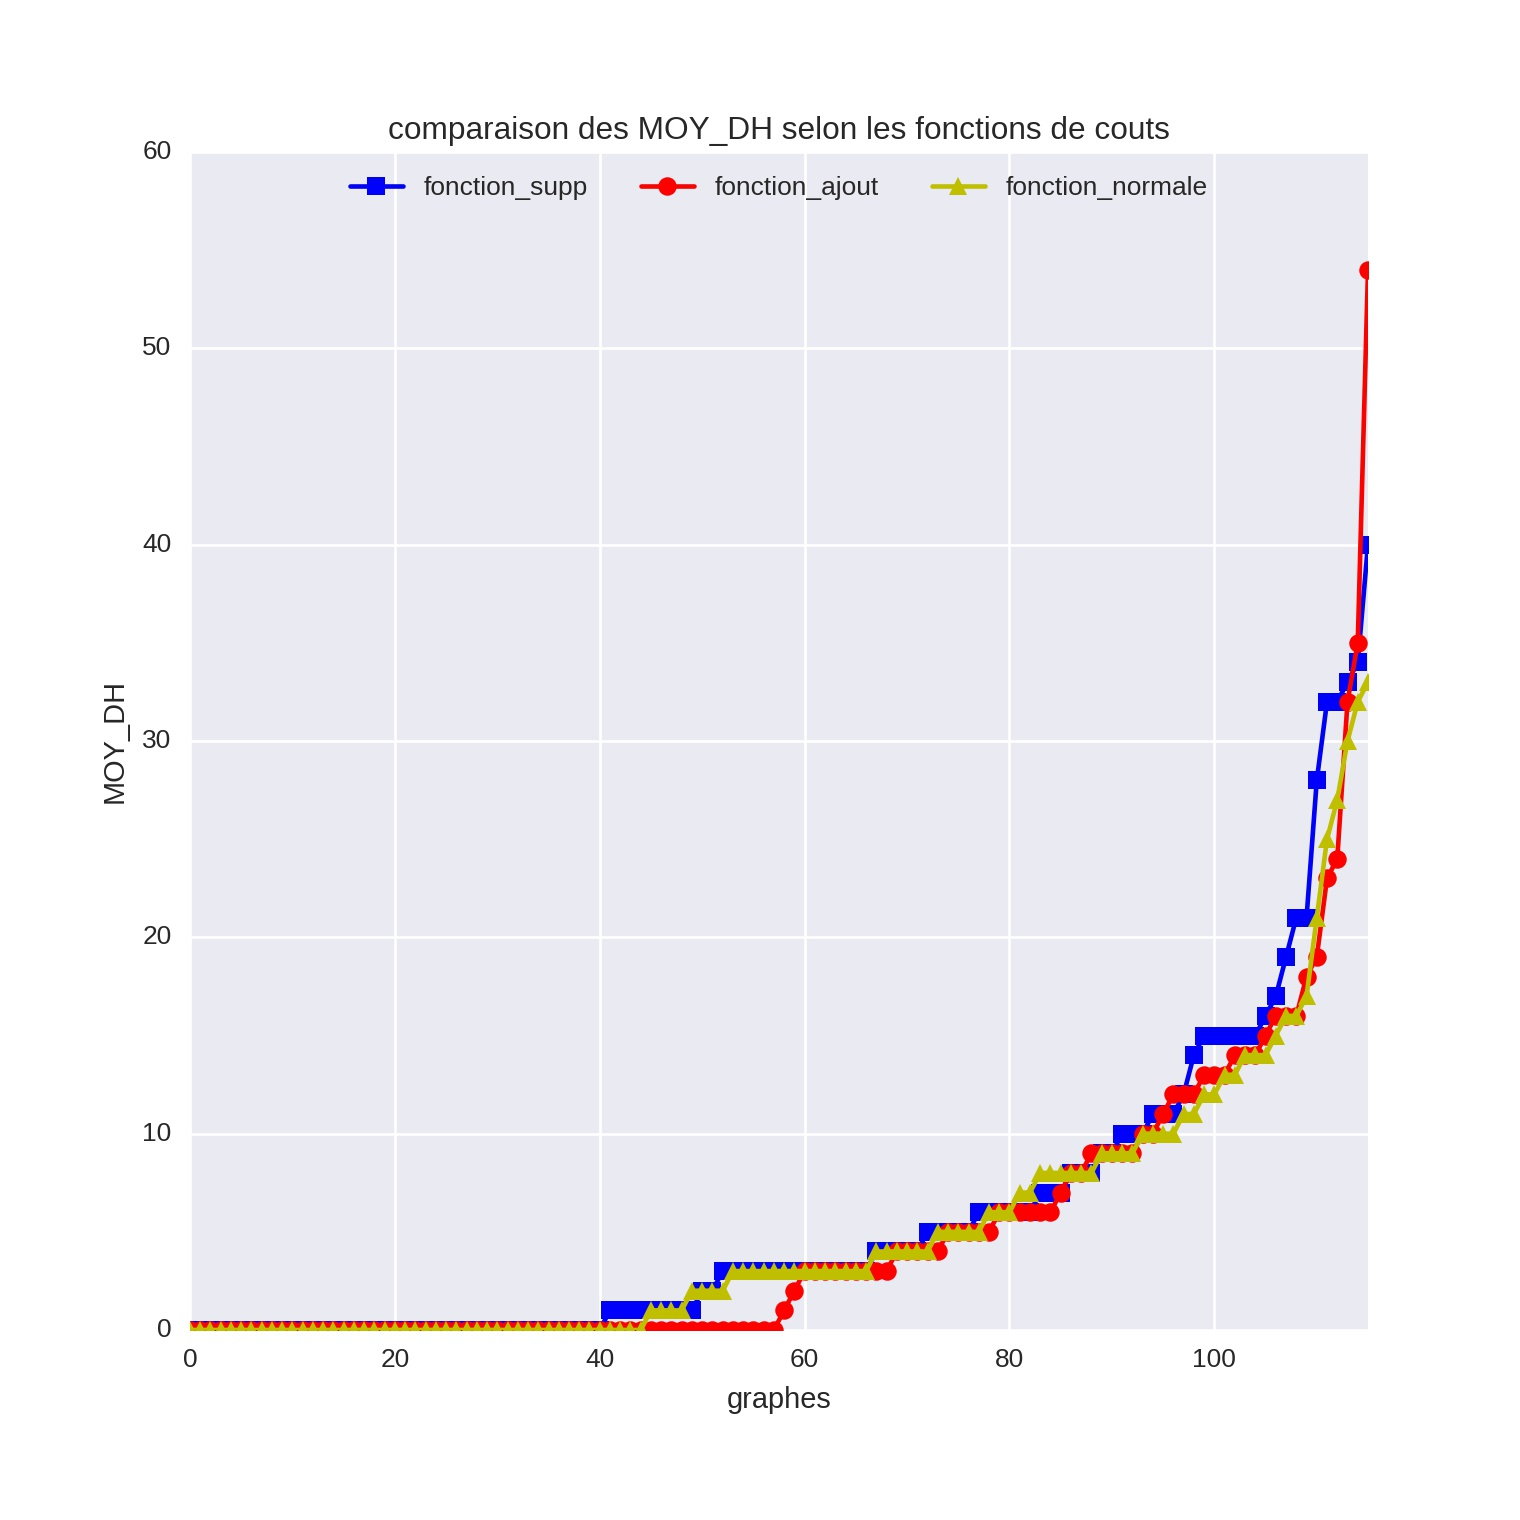
\includegraphics[scale=0.25]{comparaison_fct_couts_moy_dh_s_07_aleatoire_supp_ajout_normale.jpeg}
\caption{ Comparaison entre les fonctions de co\^ut {\em normale},  {\em ajout} et  {\em suppression} : la fonction {\em ajout} est la courbe en rouge, la fonction {\em normale} est en jaune et la fonction {\em suppression est en bleu}}
\label{comparaisonFctCoutNormaleAjoutSuppression} 
\end{figure}
 \FloatBarrier
% ----------- comparaisonFctCoutNormaleAjoutSuppression -----------------
Nous constatons que la courbe de la fonction {\em unitaire} est au dessus de celle de la fonction {\em normale} dans le graphique $(e)$ de la figure \ref{comparaisonFctCoutUnitaireNormale}.
Avec $s=0.7$, l'ensemble de cases \'erron\'ees sont des cases {\em fausses positives} (graphique $(c)$ de la figure \ref{comparaisonFctCoutUnitaireNormale}).
En appliquant les fonctions {\em unitaire} et {\em normale}, nous avons l'introduction de cases {\em fausses n\'egatives} et le nombre de ces cases est plus important dans la fonction {\em unitaire}. Ce nombre fait cro\^itre la distance de Hamming $moy\_DH$ parce que la correction a r\'eduit le nombre de cases {\em fausses positives} dans la fonction {\em normale} (voir les graphiques $(a)$ et $(c)$ de la figure  \ref{comparaisonFctCoutUnitaireNormale}).
Ce qui explique les faibles distances $moy\_DH$ de la fonction {\em normale}. La fonction {\em normale} donne de meilleurs r\'esultats et nous la choisissons dans le calcul des co\^uts de correction.
\newline

Par ailleurs, dans la figure \ref{comparaisonFctCoutNormaleAjoutSuppression}, les courbes des  fonctions  {\em normale}, {\em ajout} et {\em suppression} sont entremel\'ees et il ne se d\'egage aucun \'ecart significatif entre elles. Il est donc difficile de juger de l'influence d'une des fonctions sur la correction des sommets de $\cal C$.  
\newline 

{\bf Conclusion} :
 prioriser l'ajout \`a la suppression et vice versa n'a aucune influence sur les distances de Hamming quand nous utilisons les valeurs de corr\'elations. Toutefois,  il est pr\'ef\'erable de consid\'erer les corr\'elations dans le calcul du co\^ut de la modification d'une case parce que cela am\'eliore les distances $moy\_DH$ comme il est indiqu\'e dans le graphique $(e)$  de la figure \ref{comparaisonFctCoutUnitaireNormale}.
	\subsection{Conclusion de l'exp\'erimentation 2}	
		Nous avons g\'en\'er\'e des valeurs de corr\'elations pour toutes les cases de la matrice $M_{LG}$ en consid\'erant la distribution des valeurs de corr\'elation du r\'eseau \'electrique du data center {\em Champlan}. 
Les valeurs de corr\'elation suivent des lois normales asym\'etriques de param\`etre $\alpha = 5$ pour les cases \`a $0$ et  de param\`etre $\alpha = -5$ pour les cases \`a $1$.
La matrice de corr\'elation $M_c$ est construite \`a partir de ces corr\'elations.
Un ensemble $s \in S$ de seuils est appliqu\'e \`a la matrice $M_c$ pour la transformer en la matrice d'adjacence $M_s$ du graphe $G_s$. 
La matrice $M_s$ contient des cases {\em fausses n\'egatives} et {\em fausses positives}. 
Nous cherchons \`a minimiser la distance de Hamming en corrigeant le maximum de cases erron\'ees pendant l'algorithme de correction. Cela passe par la s\'election ad\'equate du seuil et de la fonction de co\^ut.
Apr\`es l'ex\'ecution de notre couple d'algorithmes, nous  avons d\'eduit que le bon seuil est contenu dans l'intervalle $s = ]0.6,0.7]$ et que la fonction {\em normale} est la meilleure fonction de co\^ut. 
L'utilisation du seuil $s$ et de la fonction {\em normale} ne garantissent pas la suppression totale des cases erron\'ees.  Mais elles minimisent leur nombre de telle sorte qu'un expert du m\'etier puisse effectuer les corrections manuellement qui conduisent au line-graphe $LG$ recherch\'e.
Dans la section suivante, nous nous int\'eressons aux graphes dans lesquels tous les sommets ne peuvent \^etre couverts par $1$ ou $2$ cliques. Ces graphes sont dits {\em grilles boucl\'ees}. 		

%---------------------------------------------------------------------------
%------- experimentation 3  graphes grilles boucl\'ees
%---------------------------------------------------------------------------	
\section{Exp\'erimentation 3 : algorithmes sur les grilles boucl\'ees}
	Nous consid\'erons des graphes dans lequels le voisinage d'un sommet peut \^etre couvert par  une ou deux cliques. L'ex\'ecution de l'algorithme de couverture sur chacun de ces graphes fournit une couverture vide. Cette famille de graphes est d\'esign\'ee graphes {\em grilles boucl\'ees}. Apr\`es l'ex\'ecution de l'algorithme de couverture, tous les sommets de la {\em grille boucl\'ee} sont dans l'ensemble $\cal C$ des sommets \`a corriger.
\newline
Dans cette section, nous \'evaluons les performances de nos algorithmes, particuli\`erement l'algorithme de correction en effectuant  des op\'erations de {\em suppression } et d'{\em ajout} d'ar\^etes uniquement.
Nous d\'eterminons une borne sup\'erieure de la distance line de ces graphes.
Nous comparons cette borne avec les r\'esultats obtenus par l'algorithme de correction avec l'approche {\em al\'eatoire sans remise} (voir tableau \ref{tab:recapApprocheCorrection}).
\newline
 Nous d\'ebutons notre analyse par la d\'efinition et la construction d'une grille boucl\'ee. Ensuite, nous d\'ecrivons le protocole d'exp\'erimentation sur des grilles boucl\'ees d'ordres diff\'erents. Enfin nous interpr\'etons les r\'esultats obtenus pour chaque op\'eration.
	\subsection{D\'efinition des grilles boucl\'ees et les distances line th\'eoriques}
%		Soient $k$ et $k'$ deux entiers pairs non nuls avec 
$k$ le nombre de sommets par colonnes et 
$k'$ le nombre de sommets par lignes et
$G_{k,k'}$ une grille boucl\'ee.

%Soit $G_{k,k'}$ une grille boucl\'ee de $$ laquelle $k$ et $k'$ d\'esignent le nombre de sommets  respectivement par lignes et colonnes. 
%Nous pr\'ecisons que les nombres $k$ et $k'$ sont {\em pairs}.




%Soit $G_{k,k'}$ la famille de graphes cellules dans laquelle $k$ et $k'$ d\'esignent le nombre de graphes cellules respectivement par lignes et colonnes.
%Nous pr\'ecisons que les nombres $k$ et $k'$ sont {\em impairs}.
%
%\begin{definition}
%Une cellule est un graphe biparti $K_{2,2}$ non orient\'e avec un cycle.
%\end{definition}
%
%\begin{definition}
%Le graphe $G_{1,1}$ est une cellule.
%\end{definition}
%
%% definir la cellule en fonction de n,m  n in k et m in k'
		\subsubsection{D\'efinition de la grille boucl\'ee $G_{k,k'}$ }
			Chaque sommet de $G_{k,k'}$ est identifi\'e par le couple $(i,j)$ avec $0 \le i < k$ et $0 \le j < k'$. Le sommet $(i,j)$ est adjacent  au sommet :
\begin{itemize}
	\item $(i, j+1)$ si $j < k'-2$
	\item $(i+1,j)$ si $i < k-2$
	\item $(i,j-1)$ si $j > 0$
	\item $(i-1,j)$ si $i > 0$
\end{itemize}
De plus, les sommets  $(0,0)$ et $(0,k-1)$,  $(0,0)$ et $(0,k'-1)$ , $(k-1,0)$ et $(k-1,k'-1)$, $(0,k'-1)$ et $(k-1,k'-1)$ sont adjacents.
On remarque que tout graphe  induit par un sommet et son voisinage forme un graphe \'etoile $K_{1,4}$.
La figure \ref{exempleGrapheCellule} est un exemple de {\em grille boucl\'ee} $G_{4,4}$. Ce graphe contient $16$ sommets, $28$ ar\^etes. Les sommets $(0,0), (0,1), (1,1), (1,0)$ forme une cellule et le graphe $G_{4,4}$ contient  $10$ cellules. 
% ---- figure exemple graphe cellule G_{4,4}
\begin{figure}[htb!] 
\centering
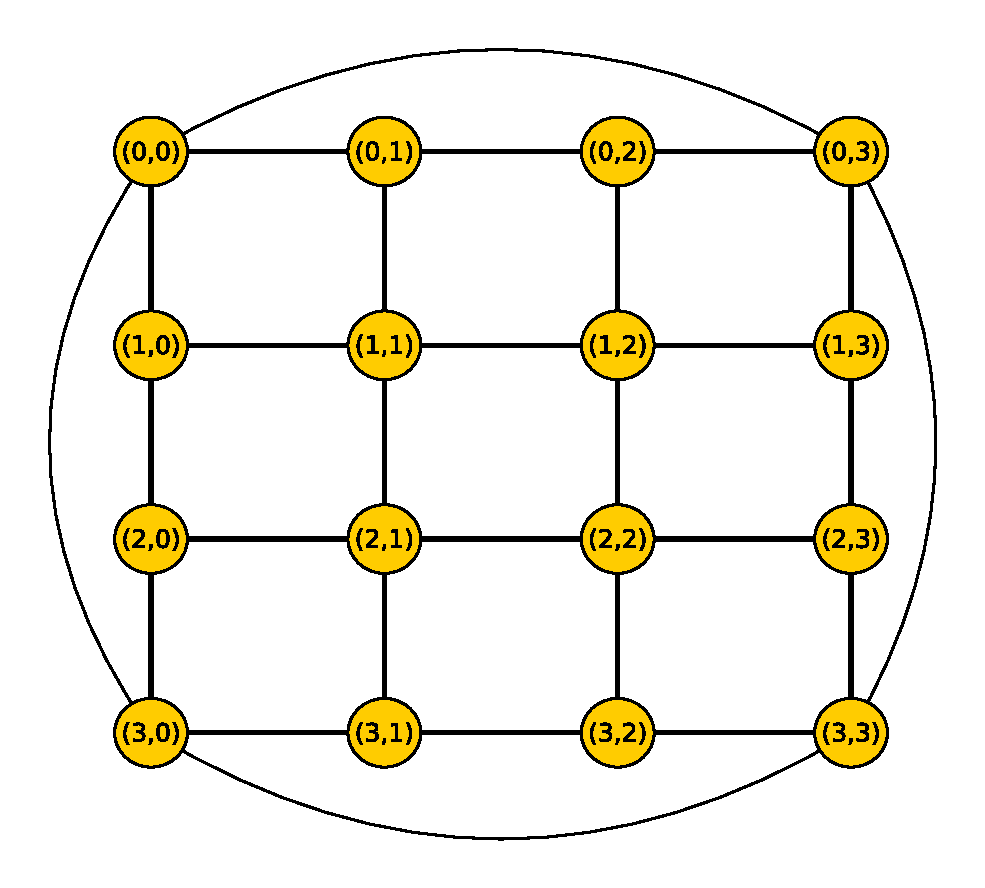
\includegraphics[scale=0.6]{exempleGrapheCelluleG33.eps}
\caption{ La grille boucl\'ee $G_{4,4}$ : elle est compos\'ee de $16$ sommets, $28$ ar\^etes et $10$ cellules. }
\label{exempleGrapheCellule} 
\end{figure}
%\FloatBarrier
% ---- figure exemple graphe cellule G_{4,4}
\begin{definition}
Une cellule est un cycle de longueur $4$ identifi\'e par les sommets $(i,j)$, $(i,j+1)$, $(i+1,j)$ et $(i+1,j+1)$ avec $i<k-1$ et $j<k'-1$. Nous notons une telle cellule $C_{i,j}$.
\end{definition}
Si $k = k' = 2$, la grille boucl\'ee $G_{2,2}$ est la cellule $C_{0,0}$.

\begin{property}
Le graphe $G_{k,k'}$ poss\`ede $k \times k'$ sommets,  $k \times (k'-1) + k' \times(k-1) + 4$  ar\^etes et $(k-1) \times (k'-1) +1$ cellules.
\end{property}

		\subsubsection{Correction des grilles boucl\'ees}
			Nous allons consid\'erer les modifications de l'ensemble des ar\^etes de $G_{k,k'}$ afin d'obtenir un line-graphe. 
La premi\`ere modification  se base uniquement par ajout d'ar\^etes et la seconde sur la suppression d'ar\^etes uniquement. 
Nous supposons que les deux op\'erations conduisent sur la m\^eme borne sup\'erieure de $DL(G_{k,k'})$.


%La grille boucl\'ee $G_{k,k'}$ ne contient aucune clique. 
%Nous appliquons l'algorithme de correction pour couvrir les sommets de ${\cal C}$  avec des cliques et que le line-graphe d\'ecoulant de cette couverture de corr\'elation soit de distance minimale. 
%Pour effectuer la correction, nous pouvons soit ajouter ou soit supprimer des ar\^etes uniquement.
%Nous simulons l'op\'eration {\em ajout uniquement} d'ar\^etes en attribuant des poids tr\`es faibles pour chaque ar\^ete ajout\'ee  et des poids tr\`es  \'elev\'es pour chaque ar\^ete supprim\'ee. De m\^eme, l'op\'eration  {\em suppression uniquement} d'ar\^etes se r\'ealise en attribuant des poids tr\`es faibles pour chaque ar\^ete supprim\'ee et des poids tr\`es  \'elev\'es pour chaque ar\^ete ajout\'ee.
%Nous allons d\'etailler les op\'erations d'ajout et de suppression d'ar\^etes pendant l'algorithme de correction. 

%Soient la fonction de co\^ut {\em ajout} qui ajoute uniquement des ar\^etes et la fonction de co\^ut {\em suppression} qui supprime uniquement des ar\^etes. 
%Nous allons d\'etailler les op\'erations d'ajout et de suppression d'ar\^etes pendant l'algorithme de correction. 

\subsubsubsection{Modification par {\em ajout d'ar\^etes uniquement}}
Soit le graphe $G_{k,k'}$ contenant $k \times k' + 1$ cellules.
Pour transformer chaque cellule en cliques comme cela est illustr\'e dans la figure \ref{exempleCorrectionGrapheCelluleAvecAjout}, nous ajoutons $2$ ar\^etes.
Nous consid\'erons le sommet $(0,0)$ contenu dans les cellules $C_{0,0}$ et $C_{k-1,k'-1}$.
Nous ajoutons $2$ ar\^etes dans $C_{0,0}$ et $C_{k-1,k'-1}$. Les cellules deviennent des cliques $K_4$. 
\newline
L'ar\^ete $\{(i,j+1),(i+1,j)\}$ appartient aux cellules  $C_{i,j}$ et  $C_{i,j+1}$.
Or cette ar\^ete est d\'ej\`a couverte par une clique $K_4$ de la cellule $C_{i,j}$.
Alors nous ne pouvons pas ajouter d'ar\^etes dans la cellule $C_{i,j+1}$.
 L'ar\^ete $\{(i,j+1),(i,j+2)\}$ forme une clique $K_2$.
 Le sommet $(i,j+1)$ est couvert par une clique $K_4$ et une clique $K_2$. 
Le sommet $(i+1,j)$ est aussi couvert par une clique $K_4$ et une clique $K_2$ parce que les cellules $C_{i,j}$ et  $C_{i+1,j}$ partagent l'ar\^ete $\{(i+1,j),(i+1,j+1)\}$  et cette ar\^ete forme une clique $K_4$ avec la cellule $C_{i,j}$.
Les cellules $C_{i,j}$ et  $C_{i+1,j+1}$ ne partagent que le sommet  $(i+1,j+1)$. En plus les ar\^etes  $\{(i+1,j+1),(i+2,j+1)\}$ de  $C_{i+1,j}$ et  $\{(i+1,j+1),(i+1,j+2)\}$ de $C_{i,j+1}$ ne sont pas couvertes par une clique $K_4$. Nous pouvons alors transformer $C_{i+1,j+1}$ en une clique $K_4$  en ajoutant $2$ ar\^etes.
\newline
Ainsi, dans des cellules successives en lignes (avec $k$) ou en colonnes (avec $k'$), nous ajoutons des ar\^etes dans $\lceil \frac{k \times k'}{2} \rceil  + 1$ cellules. 
L'ar\^ete  d'une cellule qui n'est pas contenue par une clique $K_4$ forme une clique $K_2$.
Les cellules ayant un seul sommet en commun sont transform\'ees en des cliques $K_4$. 
\newline
\`A la fin  de la correction, la grille boucl\'ee $G_{k,k'}$ est partitionn\'ee en des cliques finies $K_4$ et $K_2$.
Dans cette construction, on remarque que chaque sommet est couvert par $2$ cliques. De cette construction d\'ecoule le lemme suivant :

\begin{lemma}
La distance line d'un graphe cellule $G_{k,k'}$ avec l'op\'eration  {\em ajout uniquement} est 
\begin{equation}
DL(G_{k,k'}) \le k \times k' +3 
\end{equation}
\end{lemma}

% ---- figure exemple correction graphe cellule G_{4,4}
\begin{figure}[htb!] 
\centering
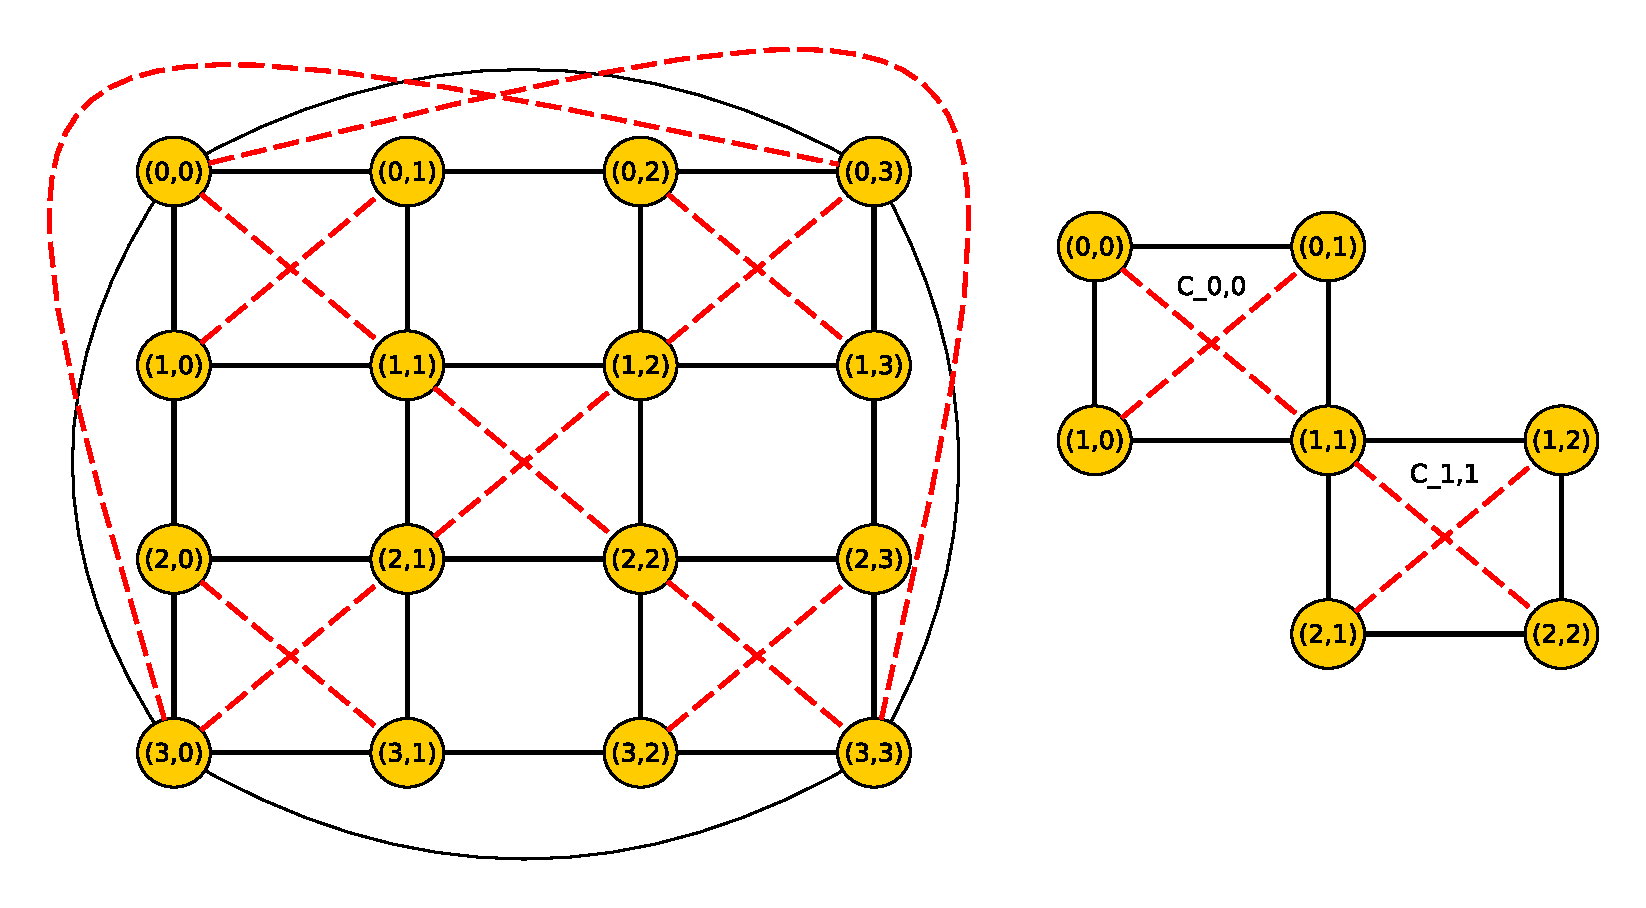
\includegraphics[scale= 0.6]{exempleGrapheCelluleAjoutG33.eps}
\caption{ La grille boucl\'ee $G_{4,4}$ : elle est compos\'ee de $16$ sommets, $33$ ar\^etes. Il contient $4$ cliques $K_{2}$ et $6$ cliques $K_4$. Les ar\^etes ajout\'ees sont les traits de couleur rouge.}
\label{exempleCorrectionGrapheCelluleAvecAjout}
\end{figure}
% ---- figure exemple correction graphe cellule G_{4,4}
Dans la figure \ref{exempleCorrectionGrapheCelluleAvecAjout}, nous r\'ealisons la correction de distance line $DL(G_{4,4})  \le 12$ en transformant les cellules partageant un sommet en cliques $K_4$. C'est le cas des cellules $C_{1,2}$ et  $C_{0,2}$ qui ont le sommet $(1,2)$ en commun. 
Les ar\^etes partag\'ees entre deux cellules ont un des sommets couvert par une clique $K_2$ et l'autre sommet couvert par une clique $K_4$. Tel est le cas avec le sommet $(3,2)$ qui forme l'ar\^ete $\{(2,2),(3,2)\}$ et cette ar\^ete est contenue par une clique $K_4$.






%
%L'ar\^ete $\{(0,1),(1,1)\}$ appartient aux cellules  $C_{0,0}$ et  $C_{0,1}$. Or cette ar\^ete est d\'ej\`a couverte par une clique $K_4$ de la cellule $C_{0,0}$. Alors nous ne pouvons pas ajouter d'ar\^etes dans la cellule $C_{0,1}$. L'ar\^ete $\{(0,1),(0,2)\}$ forme une clique $K_2$. Le sommet $(0,1)$ est couvert par une clique $K_4$ et une clique $K_2$. 
%Le sommet $(1,0)$ est aussi couvert par une clique $K_4$ et une clique $K_2$ parce que les cellules $C_{0,0}$ et  $C_{1,0}$ partagent l'ar\^ete $\{(1,0),(1,1)\}$  et cette ar\^ete forme une clique $K_4$ avec la cellule $C_{0,0}$.
%Les cellules $C_{0,0}$ et  $C_{1,1}$ ne partagent que le sommet  $(1,1)$. En plus les ar\^etes  $\{(1,1),(2,1)\}$ de  $C_{1,0}$ et  $\{(1,1),(1,2)\}$ de $C_{0,1}$ ne sont pas couverts par une clique $K_4$. Nous pouvons alors transformer $C_{1,1}$ en une clique $K_4$  en ajoutant $2$ ar\^etes .
%\newline
%Ainsi, dans des cellules successives en lignes (avec $k$) ou en colonnes (avec $k'$), nous ajoutons des ar\^etes dans une cellule sur deux. 
%%Une ar\^ete d'une cellule dans laquelle nous n'avons pas ajout\'e d'aretes devient une clique $K_2$. 
%L'ar\^ete  d'une cellule qui n'est pas contenue par une clique $K_4$ forme une clique $K_2$.
%Les cellules ayant un seul sommet en commun sont transform\'ees en des cliques $K_4$. 
%\newline
%\`A la fin  de la correction, la grille boucl\'ee $G_{k,k'}$ est partitionn\'e en des cliques $K_4$ et $K_2$.
%La distance de correction entre $G_{k,k'}$ et $L(G_{k,k'})$ est de $DC_{k,k'} = 2 \times (\lceil \frac{k \times k'}{2} \rceil  + 1)$ et cette distance est minimale.
%\begin{lemma}
%La distance line d'un graphe cellule $G_{k,k'}$ avec l'op\'eration  {\em ajout uniquement} est 
%\begin{equation}
%DL(G_{k,k'}) \le k \times k' +3 
%\end{equation}
%\end{lemma}
%\begin{proof}
%comment prouver la borne superieure?
%\end{proof}
%
%% ---- figure exemple correction graphe cellule G_{3,3}
%\begin{figure}[htb!] 
%\centering
%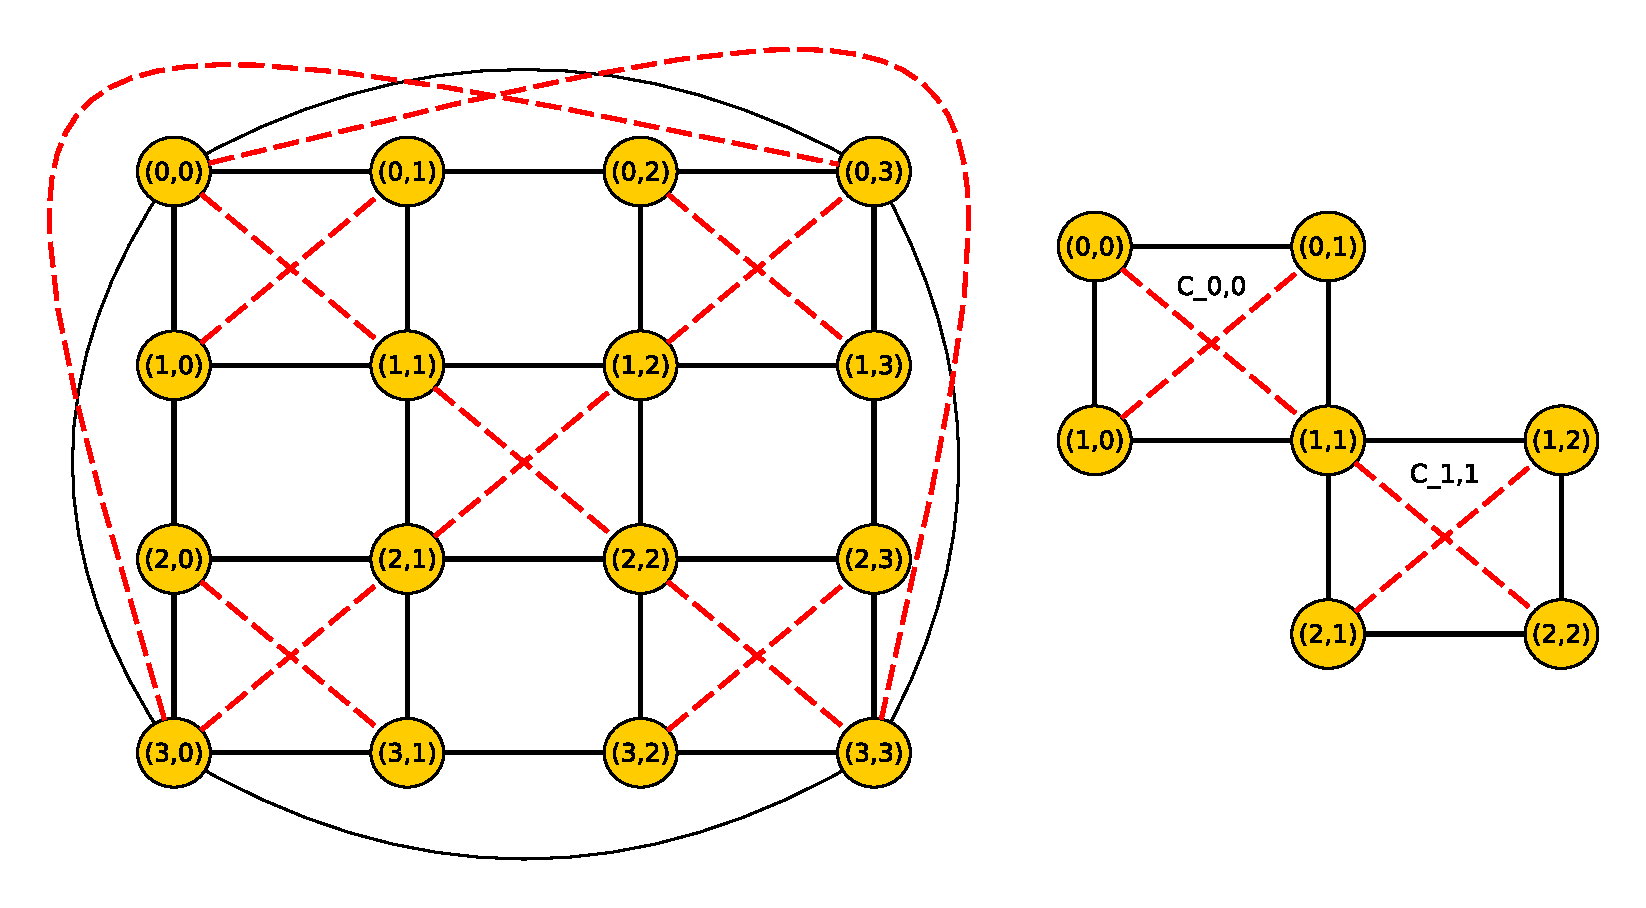
\includegraphics[scale= 0.7]{exempleGrapheCelluleAjoutG33.eps}
%\caption{ La grille boucl\'ee $G_{4,4}$ : il est compos\'e de $16$ sommets, $33$ ar\^etes. Il contient $4$ cliques $K_{2}$ et $6$ cliques $K_4$. Les ar\^etes ajout\'ees sont les traits de couleur rouge.}
%\label{exempleCorrectionGrapheCelluleAvecAjout}
%\end{figure}
%% ---- figure exemple correction graphe cellule G_{3,3}
%Dans la figure \ref{exempleCorrectionGrapheCelluleAvecAjout}, nous r\'ealisons la correction de distance line $DL(G_{4,4})=12$ minimale en transformant les cellules partageant un sommet en cliques $K_4$. C'est le cas des cellules $C_{1,2}$ et  $C_{0,2}$ qui ont le sommet $(1,2)$ en commun. 
%Les ar\^etes partag\'ees entre deux cellules ont un des sommets couvert par une clique $K_2$ et l'autre sommet couvert par une clique $K_4$. Tel est le cas avec le sommet $(3,2)$ qui forme l'ar\^ete $\{(2,2),(3,2)\}$ et cette ar\^ete est contenue par une clique $K_4$.

\subsubsubsection{Modification par {\em suppression d'ar\^etes uniquement}}
\label{modificationSuppressionAretesUniquement}
Soit le graphe $G_{k,k'}$ contenant $k \times k' + 1$ cellules.
Nous supprimons les ar\^etes \\ $[\{(0,0),(k-1,0) \},  \{(0,0),(0, k'-1) \}, \{(k-1,0),(k-1,k'+1) \}]$ de la  cellule $C_{k-1,k'-1}$. Cette cellule contient uniquement  l'ar\^ete $\{(0,k'-1),(k-1,k'-1) \}$ et cette ar\^ete forme la clique $K_2$.
Nous supprimons \'egalement les ar\^etes $\{(0,k'-2),(0,k'-1)\}$ et $\{(k-2,k'-1),(k-1,k'-1) \}$  incidentes respectivement aux sommets $(0,k'-1)$ et $(k-1,k'-1)$ de sorte que ces sommets soient couverts par deux cliques $K_2$.
Les sommets de degr\'e minimums $(0,0)$, $(k-1,0)$. Ils sont couverts par deux cliques $K_2$ c'est-\`a-dire $\{(0,0),(1,0)\}$ et $\{(k-2,0) ,(k-1,0)\}$.
\newline
Consid\'erons les sommets de degr\'e $4$. Soit $(i,j)$ un tel sommet.
Pour former une bipartition autour de ce sommet, nous allons supprimer $2$ ar\^etes. Chaque ar\^ete appartient \`a deux cellules voisines. Dans notre cas, nous supprimons l'ar\^ete $\{(i-1, j), (i,j)\}$ entre les cellules $C_{i-1,j-1}$ et $C_{i-1,j}$ et aussi l'ar\^ete $\{(i,j), (i+1,j)\}$ entre les cellules $C_{i,j-1}$ et $C_{i,j}$. Ces sommets sont couverts aussi par des cliques $K_2$.
\newline
Les ar\^etes incidentes \`a un sommet de degr\'e $3$ et n'\'etant pas des cliques $K_2$ sont aussi supprim\'ees.
\newline
\`A la fin de l'algorithme de correction, la couverture de corr\'elation ne contient que des cliques $K_2$.
Le graphe $G_{k,k'}$ est un cycle hamiltonien de taille $(k \times k'+1) + k' + 1$.
La distance de correction entre $G_{k,k'}$ et $L(G_{k,k'})$ est $DC_{k,k'} = k \times k' +3 $ et cette distance est minimale.

\begin{lemma}
La distance line  d'une grille boucl\'ee $G_{k,k'}$ avec l'op\'eration {\em suppression uniquement} d'ar\^etes est 
\begin{equation}
\label{borneSuperieureDL}
DL(G_{k,k'}) = k \times k' +3 
%DL_{supp}(G_{k,k'}) = k \times (k' +1) ===> cela correspond a quoi?
\end{equation}
\end{lemma}

% ---- figure exemple correction graphe cellule G_{3,3}
\begin{figure}[htb!] 
\centering
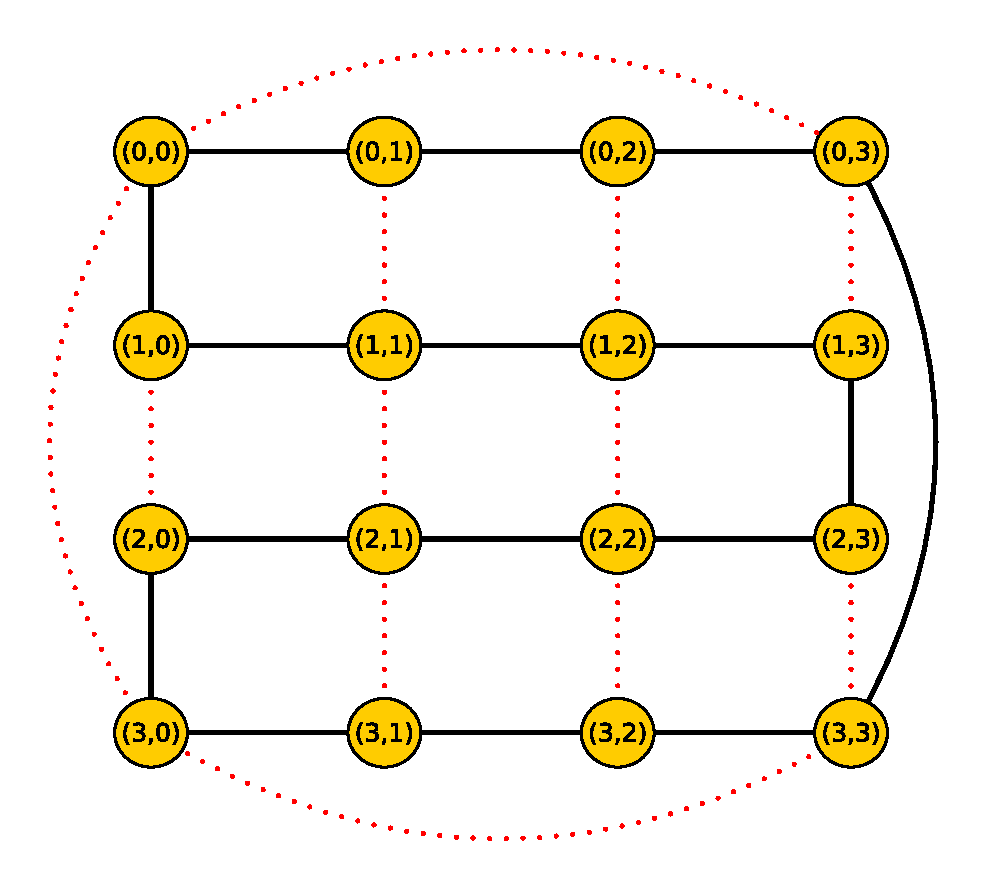
\includegraphics[scale = 0.7]{exempleGrapheCellulesSuppressionG33.eps}
\caption{ La grille boucl\'ee $G_{4,4}$ : elle est compos\'ee de $16$ sommets, $16$ ar\^etes et $16$ cliques $K_2$. Les ar\^etes supprim\'ees sont les traits en pointill\'ees rouges }
\label{exempleCorrectionGrapheCelluleAvecSuppression}
\end{figure}
%\FloatBarrier
% ---- figure exemple correction graphe cellule G_{3,3}
Une illustration de la correction avec l'op\'eration {\em suppression uniquement} est faite avec la grille $G_{4,4}$ dans la figure \ref{exempleCorrectionGrapheCelluleAvecSuppression}.
La grille $G_{4,4}$ poss\`ede $ k \times k' = 16$ cliques $K_2$ et $12$ ar\^etes sont supprim\'ees.
\newline

% conclusion
%Nous avons d\'etermin\'e les distances line th\'eoriques selon les fonctions de co\^ut lors de la correction de sommets de graphes cellules. Nous allons v\'erifier si les distances line obtenues exp\'erimentalement convergent vers les distances line th\'eoriques.
{\bf Conclusion} :
nous avons d\'etermin\'e deux types de modifications d'ar\^etes qui ont une borne sup\'erieure de la distance line pour chaque op\'eration. En revanche, les cliques formant la couverture de corr\'elation sont diff\'erentes selon la modification. Dans la modification {\em ajout d'ar\^etes uniquement}, le grille boucl\'e $G_{k.k'}$ contient des cliques $K_4$ et $K_2$ alors que  $G_{k.k'}$ ne contient que des cliques $K_2$ dans la {\em suppression d'ar\^etes uniquement}. 



%Nous remarquons que ces bornes  sont identiques. La distance line th\'eorique est alors born\'ee par $k \times k' +3$ quelque soit l'op\'eration de correction effectu\'ee.
%Nous allons v\'erifier si les distances de correction, obtenues apr\`es la correction des grilles boucl\'ees,  convergent vers la borne des distances line th\'eoriques.
%
%
%

	\subsection{Protocole d'exp\'erimentation sur les grilles boucl\'ees}
		Nous allons comparer cette borne sup\'erieure de l'\'equation \ref{borneSuperieureDL} avec les distances de correction obtenues par l'algorithme de correction.
\newline
Consid\'erons $G_{k,k'}$ une grille boucl\'ee dans laquelle le nombre de sommets par lignes est identique le nombre de sommets par colonnes ($k = k'$). Nous le notons $G_k$.
\newline
Nous construisons $48$ grilles boucl\'ees  contenant chacune $k \times k +1$ cellules, avec $k \in \{2,\cdots,98\}$ un nombre pair.
Dans chaque graphe $G_k$, nous ex\'ecutons   $50$ fois notre couple d'algorithmes avec chaque modification d'ar\^etes et la distance de correction obtenue est compar\'ee avec la borne sup\'erieure (\'equation \ref{borneSuperieureDL}).
\newline

Soient $\phi^{+}(u,v)$ le co\^ut de l'op\'eration {\em ajouter une ar\^ete} et 
$\phi^{-}(u,v)$ le poids de l'op\'eration {\em supprimer une ar\^ete} (voir section \ref{algorithmeCorrection}). 
\newline
La modification {\em ajout d'ar\^etes uniquement} est telle que 
\begin{itemize}
	\item L'ajout d'ar\^etes a un co\^ut  $\phi^{+}(u,v) = 1$,
	\item La suppression d'ar\^etes a un co\^ut  $\phi^{-}(u,v) = 10$.
\end{itemize}
Quant \`a la modification {\em suppression d'ar\^etes uniquement}, elle se d\'efinit comme suit :
\begin{itemize}
	\item L'ajout d'ar\^etes a un co\^ut  $\phi^{+}(u,v) = 10$.
	\item La suppression d'ar\^etes a un co\^ut  $\phi^{-}(u,v) = 1$.
\end{itemize}
Nous allons comparer l'\'evolution des distances de correction des $48$ graphes en fonction la borne sup\'erieure pour chaque modification r\'ealis\'ee.

%
%Consid\'erons $G_{k,k'}$ une grille boucl\'ee dans lequel le nombre de sommets par lignes est identique le nombre de sommets par colonnes ($k = k'$). Nous notons $G_k$ pour d\'esigner $G_{k,k'}$ et $G_k$ contient $k \times k +1$ cellules.
%Nous construisons $48$ grilles boucl\'ees dans lesquels chaque graphe contient $k \times k +1$ cellules $k \in \{2,\cdots,98\}$.
%Dans chaque graphe $G_k$, nous ex\'ecutons  notre couple d'algorithmes $50$ fois puis nous r\'ecup\'erons la distance de correction  minimale entre $G_k$ et les line-graphes $L(G_k)$ propos\'ees.
%Nous utilisons la   distance de correction  minimale parce qu'il est impossible de trouver la bonne permutation qui minimise cette distance \`a cause de la combinatoire factorielle de l'ensemble $\cal C$.
%\newline
%Soient $\phi^{+}(u,v)$ le poids de l'op\'eration {\em ajouter une ar\^ete} et $\phi^{-}(u,v)$ le poids de l'op\'eration {\em supprimer une ar\^ete}. 
%L'op\'eration {\em ajout uniquement} d'ar\^etes est telle que  $\phi^{+}(u,v) = 1$ pour l'ajout de l'ar\^ete $(u,v)$ et $\phi^{-}(u,v) = 10$ pour la suppression de l'ar\^ete $(u,v)$.
%De m\^eme,  L'op\'eration {\em suppression uniquement} d'ar\^etes est telle que  $\phi^{+}(u,v) = 10$ pour l'ajout de l'ar\^ete $(u,v)$ et $\phi^{-}(u,v) = 1$ pour la suppression de l'ar\^ete $(u,v)$.
%L'objectif de notre exp\'erimentation est de comparer l'\'evolution des distances de correction obtenues apr\`es la correction des grilles boucl\'ees par rapport aux bornes sup\'erieures des distances line th\'eoriques. 

%Nous d\'efinissons les fonctions de co\^ut {\em ajout} et {\em suppression} comme suit :
%\begin{enumerate}[label = (\alph*)]
%%\item {\em unitaire} : ajouter et supprimer une ar\^ete ont un poids $1$ ($\phi^{+} = \phi^{-} = 1$).
%\item {\em ajout} : nous donnons un poids minimal \`a l'op\'eration ``ajouter d'ar\^etes''. Ainsi nous attribuons un poids $\phi^{+} = 1$ pour l'ajout d'ar\^etes et un poids $\phi^{-} = 10$ pour la suppression d'ar\^etes.
%\item {\em suppression} : Ici nous faisons l'op\'eration inverse en donnant un poids maximal \`a l'op\'eration d'ajout d'ar\^etes. Ainsi, l'ajout d'une ar\^ete a un poids $\phi^{+} = 10$ alors que la suppression a un poids $\phi^{-} = 1$.
%\end{enumerate}
%L'objectif de notre exp\'erimentation est de comparer les distances lines th\'eoriques avec celles obtenus avec l'utilisation des fonctions de co\^uts mentionn\'ees ci-dessus.


%Nous allons comparer les diff\'erentes fonctions de co\^ut en utilisant les distances line calcul\'ees. Les courbes croissantes dans les figures \ref{priorAjout1Ajout10}, \ref{priorAjout1Supp10} et \ref{priorAjout1Supp1} s'explique par le fait que les distances line sont rang\'ees par ordre croissant.
	\subsection{Analyse des r\'esultats}
		% ---- figure comparaison_distances_line_graphes_cellules_k_2x50
%\begin{figure}[htb!] 
%\centering
%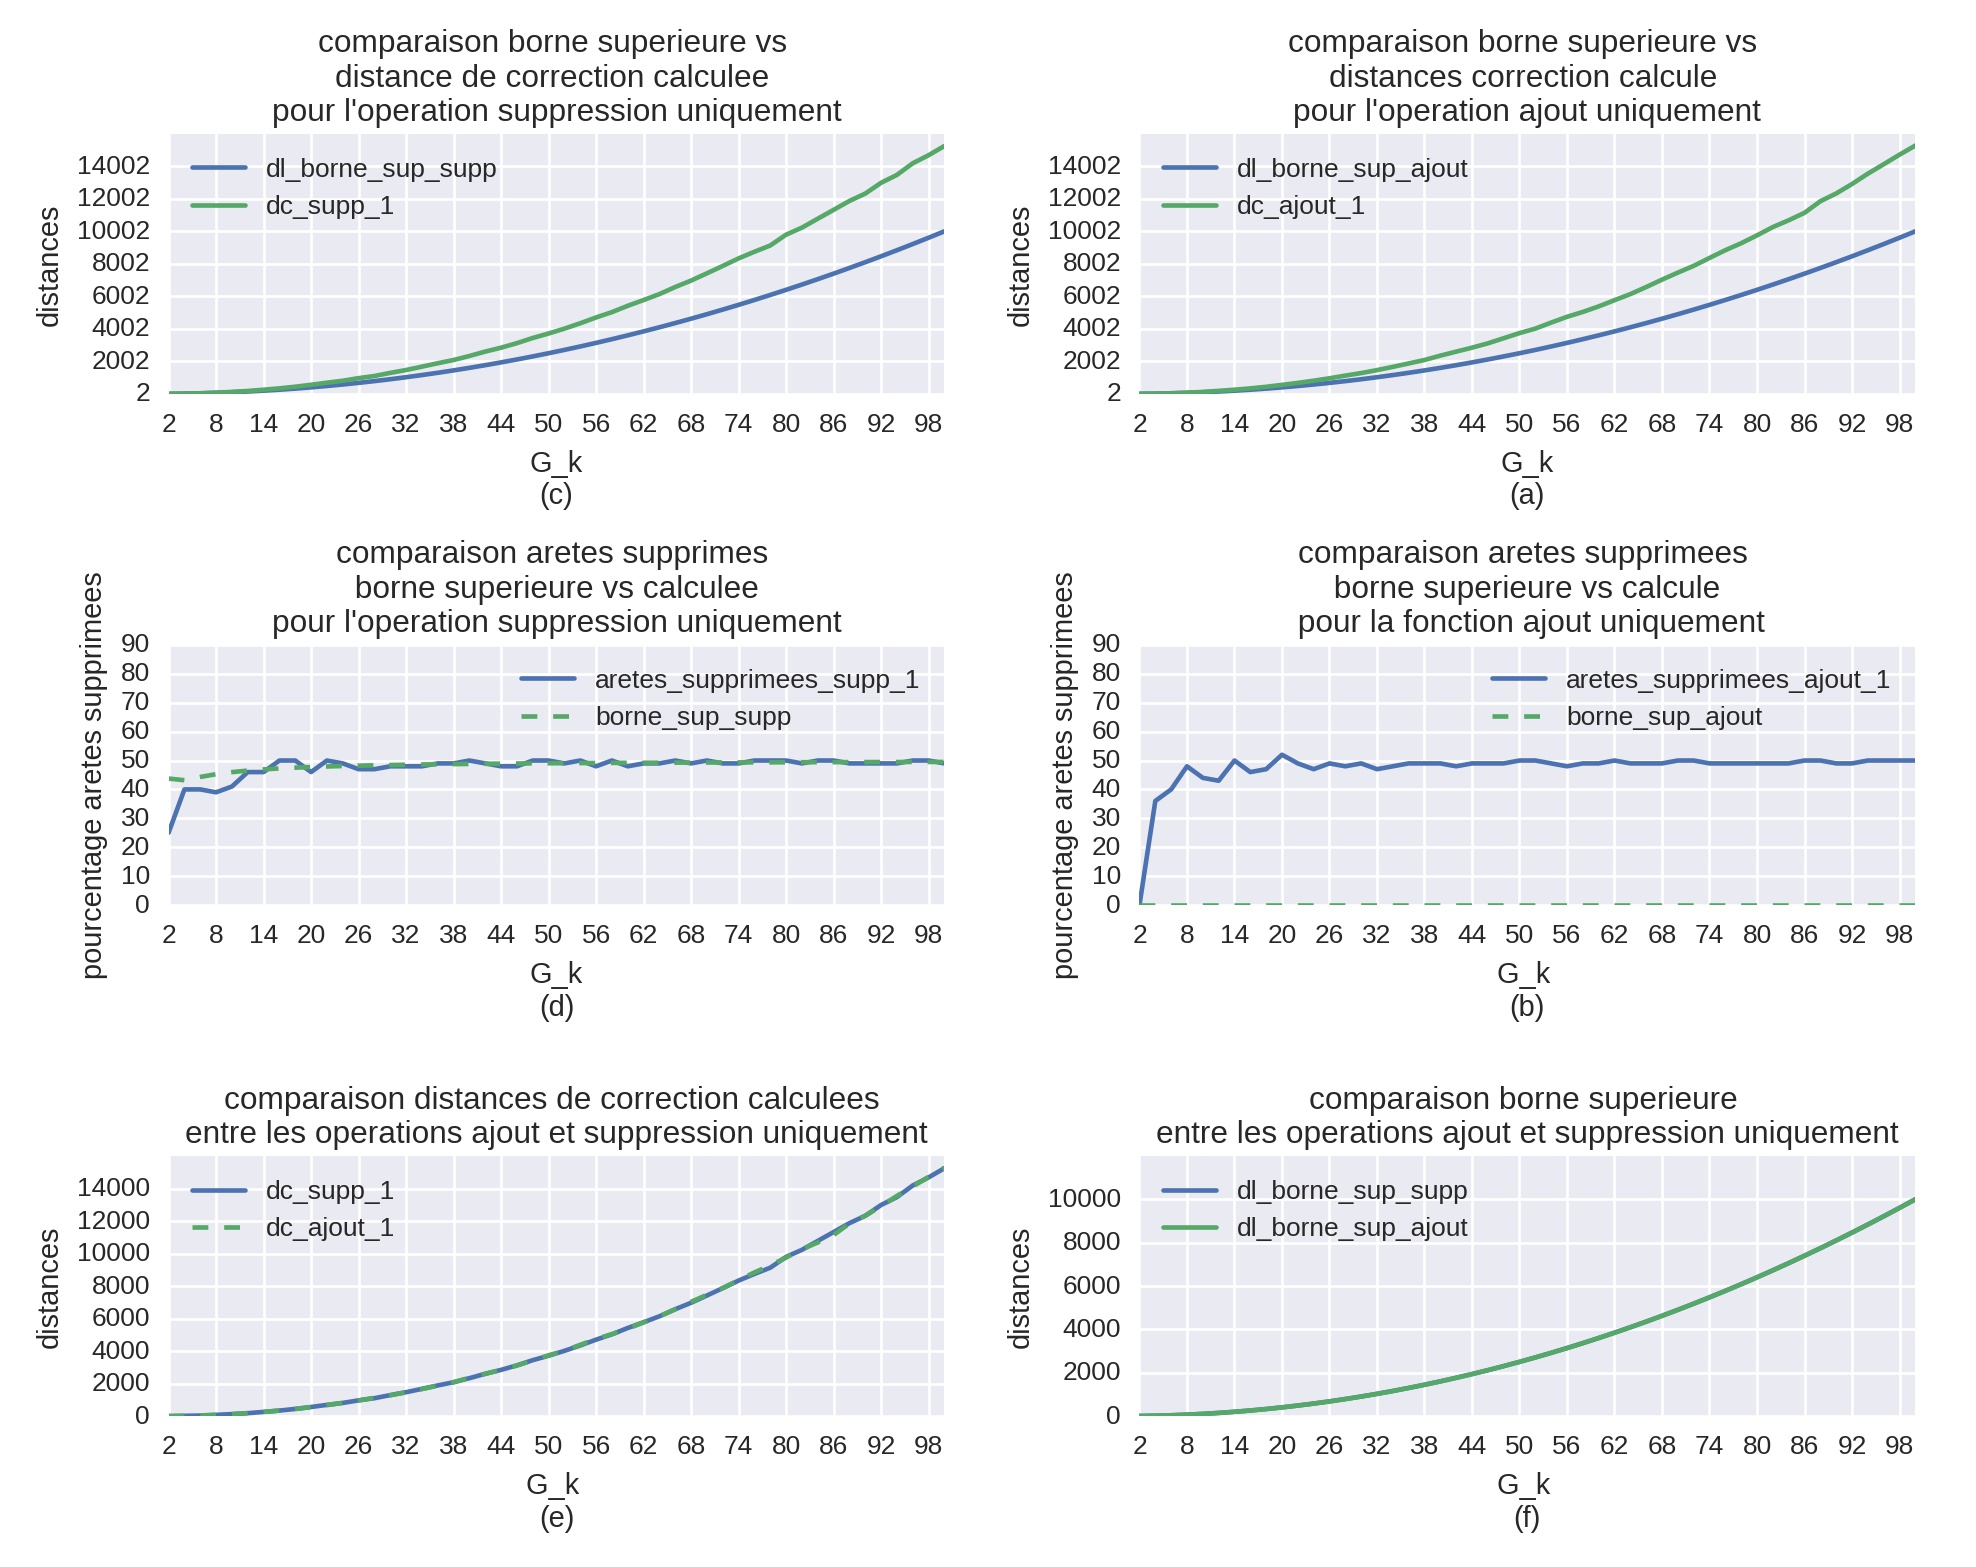
\includegraphics[scale = 0.25]{comparaison_distances_line_graphes_cellules_k_2x50.jpeg}
%\caption{Comparaison de distances lines th\'eoriques et calcul\'ees selon des fonctions de co\^ut {\em suppression} et  {\em ajout}.
%La figure $(a)$ d\'esigne la comparaison entre les distances de correction et la borne sup\'erieure de l'\'equation \ref{borneSuperieureDL} avec la modification {\em ajout d'ar\^etes uniquement}, 
%La figure $(c)$ d\'esigne la comparaison entre les distances de correction et la borne sup\'erieure de l'\'equation \ref{borneSuperieureDL} avec la modification {\em suppression d'ar\^etes uniquement}, 
%La figure $(b)$ compare le pourcentage d'ar\^etes supprim\'ees  dans les graphes boucl\'ees avec celui de la borne sup\'erieure de l'\'equation \ref{borneSuperieureDL} dans la modification {\em ajout d'ar\^etes uniquement}, 
%La figure $(d)$ compare le pourcentage d'ar\^etes supprim\'ees  dans les graphes boucl\'ees avec celui de la borne sup\'erieure de l'\'equation \ref{borneSuperieureDL} dans la modification {\em suppression d'ar\^etes uniquement},
%La figure $(e)$ compare les distances de correction entre les diff\'erentes modifications.
%}
%\label{comparaison_distances_line_graphes_cellules_k_2x50}
%\end{figure}
%\FloatBarrier
\begin{figure}[htb!] 
\centering
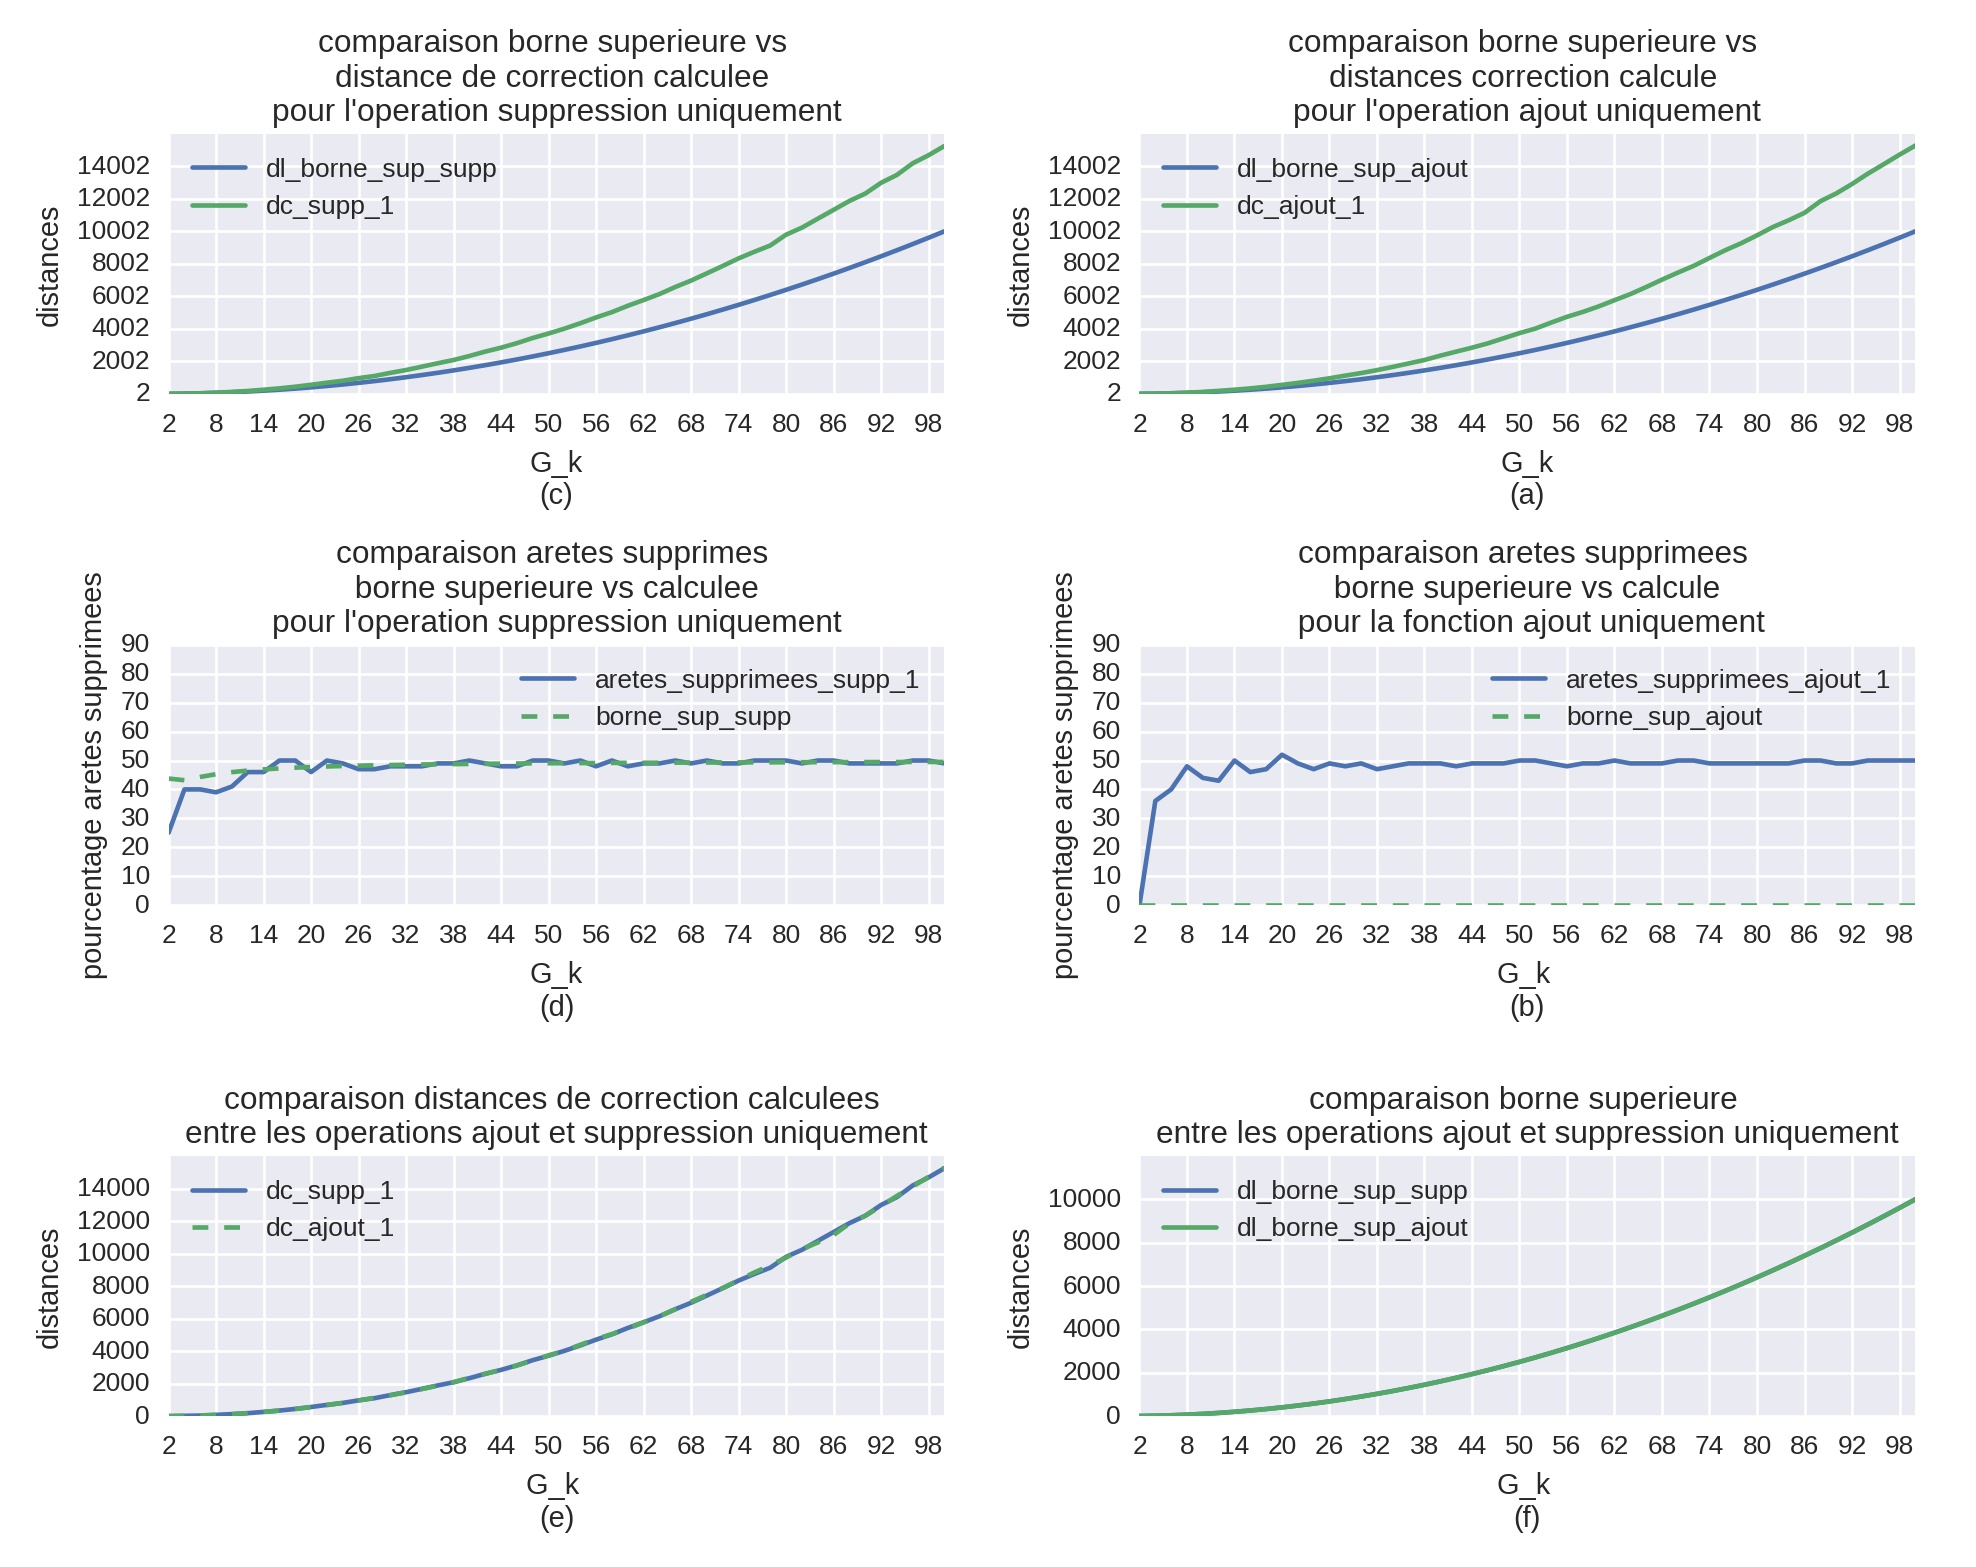
\includegraphics[scale = 0.25]{comparaison_distances_line_graphes_cellules_k_2x50.jpeg}
\caption{Comparaison entre la borne sup\'erieure de la distance line et les distances de correction calcul\'ees selon des fonctions de co\^ut {\em suppression} et  {\em ajout} : 
la figure $(a)$ d\'esigne la comparaison entre les distances de correction et la borne sup\'erieure de l'\'equation \ref{borneSuperieureDL} avec la modification {\em ajout d'ar\^etes uniquement}, 
la figure $(c)$ d\'esigne la comparaison entre les distances de correction et la borne sup\'erieure de l'\'equation \ref{borneSuperieureDL} avec la modification {\em suppression d'ar\^etes uniquement}, 
la figure $(b)$ compare le pourcentage d'ar\^etes supprim\'ees  dans les graphes boucl\'ees avec celui de la borne sup\'erieure de l'\'equation \ref{borneSuperieureDL} dans la modification {\em ajout d'ar\^etes uniquement}, 
la figure $(d)$ compare le pourcentage d'ar\^etes supprim\'ees  dans les graphes boucl\'ees avec celui de la borne sup\'erieure de l'\'equation \ref{borneSuperieureDL} dans la modification {\em suppression d'ar\^etes uniquement},
la figure $(e)$ compare les distances de correction entre les diff\'erentes modifications.
}
\label{comparaison_distances_line_graphes_cellules_k_2x50}
\end{figure}
%\FloatBarrier
% ---- figure comparaison_distances_line_graphes_cellules_k_2x50


Notre objectif est de pr\'esenter les variations des distances de correction par rapport \`a la borne sup\'erieure de la distance line pour chaque modification r\'ealis\'ee sur les graphes pendant l'algorithme de correction. Pour ce faire, nous regroupons notre analyse en $5$ exp\'erimentations.
\newline

Les deux premi\`eres exp\'erimentations comparent les distances de correction avec la borne sup\'erieure pour la modification {\em ajout d'ar\^etes uniquement} (figure \ref{comparaison_distances_line_graphes_cellules_k_2x50} (a) et 
pour la modification {\em suppression d'ar\^etes uniquement} figure \ref{comparaison_distances_line_graphes_cellules_k_2x50} (c).
Nous constatons que les courbes des distances de correction et celle de la borne sup\'erieure sont croissantes. 
La courbe de la borne sup\'erieure, d\'esign\'ee par $borneSup$ dans les graphiques $(a)$ et $(c)$, \'evolue lentement par rapport aux courbes des distances et l'\'ecart entre ces courbes croit lin\'eairement. 
Pour comprendre cet \'ecart croissant, nous v\'erifions le pourcentage d'ar\^etes  supprim\'ees pour chaque modification.  Ce sont les deux autres exp\'erimentations faites et repr\'esent\'ees par la figure 
\ref{comparaison_distances_line_graphes_cellules_k_2x50} (b) pour la modification {\em ajout d'ar\^etes uniquement} et
 la figure \ref{comparaison_distances_line_graphes_cellules_k_2x50} (d) pour la modification 
{\em suppression d'ar\^etes uniquement}. 
En effet, nous avons choisi les ar\^etes supprim\'ees parce que le nombre d'ar\^etes est d\'ej\`a connu c'est-\`a-dire $0$ pour l'ajout uniquement et la borne sup\'erieure pour la suppression uniquement. 
\newline
Nous remarquons que les ar\^etes   de $G_k$ supprim\'ees avoisinent en moyenne de
$40\%$ quand le nombre $k$ de cellules est faible ($k \le 14$) dans la modification {\em ajout ar\^etes uniquement}. Au d\'el\`a de $ k > 14 $, une ar\^ete sur deux du graphe $G_{k}$ est supprim\'ee. La courbe  $aretes\_supprimees\_ajout\_1$ dans le graphique $(b)$ repr\'esente le pourcentage d'ar\^etes supprim\'ees.  
En effet, nous expliquons ces chiffres  par l'ajout d'ar\^etes entre des sommets de cellules voisines et ces sommets ne sont pas partag\'es entre les cellules voisines. Ces ar\^etes ajout\'ees impliquent la suppression des ar\^etes de $G_k$ parce que la partition $\pi_s$ (voir section \ref{algorithmeCorrection}) des ar\^etes \`a supprimer pendant la compression n'est pas vide et contient des ar\^etes de $G_k$ en g\'en\'eral. Ainsi ces ar\^etes provoquent l'abandon des ar\^etes diagonales  ajout\'ees \`a partir du sommet commun entre des cellules comme indiqu\'e dans l'exemple du graphe $G_{4,4}$ dans la figure \ref{exempleCorrectionGrapheCelluleAvecAjout}.
\newline
En ce qui concerne la modification {\em suppression d'ar\^etes uniquement}, les ar\^etes supprim\'ees proviennent aussi des cellules voisines. 
Dans les cellules partageant un sommet, l'algorithme ajoute g\'en\'eralement une ar\^ete diagonale \`a partir de ce sommet commun dans une seule cellule. Les ar\^etes diagonales ajout\'ees sont responsables de l'augmentation de la distance de correction (courbe {\em dc\_supp\_1} dans le graphique $(c)$).
Pour des cellules partageant une ar\^ete, l'algorithme supprime certaines ar\^etes communes comme indiqu\'e dans la section \ref{modificationSuppressionAretesUniquement}. Les autres ar\^etes communes non supprim\'ees sont dues \`a la pr\'esence des ar\^etes diagonales. Cela explique pourquoi nous avons en moyenne $50\%$ des ar\^etes de $G_k$ qui sont supprim\'ees dans le graphique $(d)$. Ce pourcentage est identique \`a celui des ar\^etes supprim\'ees de la borne sup\'erieure lorsque le nombre de cellules devient \'elev\'e $k \ge 18$ et il ne signifie pas que l'algorithme de correction supprime les ar\^etes de la section \ref{modificationSuppressionAretesUniquement}.
\newline
Par ailleurs, les courbes {\em dc\_ajout\_1} de la modification d'{\em ajout d'ar\^etes uniquement} et celle {\em dc\_supp\_1}  de la modification {\em suppression d'ar\^etes uniquement} ont les m\^emes tendances et sont superpos\'ees (figure $(e)$) parce que  dans la modification d'{\em ajout}, l'algorithme ajoute la m\^eme proportion d'ar\^etes qu'il supprime dans  la modification {\em suppression}. 
\newline

\vspace{-0.25cm}
{\bf Conclusion} :   
l'exp\'erimentation montre que le line-graphe $L(G_k)$ propos\'e par l'algorithme de correction pour un $k$ donn\'ee est identique en terme de distance de correction quelle que soit la modification r\'ealis\'ee comme illustre la figure \ref{comparaison_distances_line_graphes_cellules_k_2x50}(e).
Toutefois, les graphes corrig\'es ne sont pas optimaux en terme de distances de correction parce que l'algorithme priorise dans certains cas les modifications {\em ajout d'ar\^etes uniquement} et {\em suppression uniquement} et cela leur permet d'atteindre des minimums locaux. Cependant le minimum global n'est pas atteint g\'en\'eralement. 


	\subsection{Conclusion de l'exp\'erimentation 3}
		
Les grilles boucl\'ees ont la particularit\'e d'avoir des ar\^etes qui ne peuvent \^etre partitionn\'ees en cliques. 
Nous avons d\'ecrit la construction de ces graphes et nous d\'efinissons deux m\'ethodes pour les corriger. La premi\`ere m\'ethode est la modification d'{\em ajout uniquement} qui consiste \`a ajouter uniquement des ar\^etes  et la seconde m\'ethode est la modification {\em suppression uniquement} qui supprime uniquement des ar\^etes des grilles boucl\'ees. 
Avec ces m\'ethodes, nous avons trouv\'e une borne sup\'erieure unique de la distance line des  grilles boucl\'ees et nous avons compar\'e cette borne sup\'erieure avec les distances de correction obtenues apr\`es l'algorithme de correction.
\newline
Nous remarquons que les distances de correction varient tr\`es peu entre les modifications {\em ajout uniquement} et {\em suppression uniquement}.  Les graphes corrig\'es n'ont pas de distances de corrections optimales parce que l'algorithme supprime des ar\^etes pendant la modification {\em ajout d'ar\^etes uniquement} et ajoute des ar\^etes pendant la modification {\em suppression uniquement}.  

%et ces distances ne convergent pas vers les distances th\'eoriques parce qu'il ajoute des ar\^etes dans l'op\'eration {\em suppression uniquement} et supprime des ar\^etes dans l'op\'eration {\em ajout uniquement}.  Par ailleurs, les distances line th\'eoriques sont identiques quelques soient les op\'erations car les expressions litt\'erales de ces distances  ont le m\^eme d\^egre de polyn\^omes et les coefficents de ces polyn\^omes sont tr\`es proches.

%---------------------------------------------------------------------------
%------- conclusion chapitre
%---------------------------------------------------------------------------
	\section{Conclusion du chapitre \ref{chapitreEvaluation}}
		% conclusion generale 
Le chapitre \ref{chapitreEvaluation} analyse les performances de nos algorithmes de couverture et de correction selon $3$ exp\'erimentations. 

% experimentation 1
La premi\`ere exp\'erimentation consiste \`a modifier les $k$ cases de la matrice d'adjacence du line-graphe d'un r\'eseau \'electrique. Ces cases modifi\'ees sont divis\'ees en deux sous-ensembles disjoints (cases {\em fausses n\'egatives} et cases {\em fausses positives}) selon une variable $p \in [0,1]$. Si $p = 0$ alors l'ensemble des cases modifi\'ees est compos\'e que de cases  {\em fausses positives} et si $p=1$ alors nous avons que des cases {\em fausses n\'egatives}. 
Le but est de borner le nombre de cases corrig\'ees par nos algorithmes.
Ainsi, nous avons d\'efini les distances de correction et de Hamming. 
La distance de correction est le nombre minimum de cases \`a modifier dans un graphe de $k$ cases erron\'ees pour en faire un line-graphe. 
Quant \`a la distance de Hamming, elle est la diff\'erence de cases entre les matrices de line-graphe propos\'e par nos algorithmes et le line-graphe du r\'eseau \'electrique.
Nous avons compar\'e le nombre de cases corrig\'ees avec $5$ approches de correction qui sont : {\em al\'eatoire sans remise $(2c)$}, {\em degr\'e minimun sans remise $(2a)$}, {\em co\^ut minimum sans remise $(2b)$}, {\em degr\'e minimun avec remise $(1a)$}, {\em co\^ut minimum avec remise $(1b)$}. \`A chaque approche, nous avons $3$ co\^uts de modification  d'une case : {\em unitaire}, {\em ajout} et {\em suppression}.
Nous avons conclut que l'approche  {\em al\'eatoire sans remise $(2c)$} proposait des distances de correction minimales quelle que soit la repartition effectu\'ee $p$ et la fonction de co\^ut utilis\'ee. Ces distances constituent la borne sup\'erieure de la distance line quand le nombre $k$ de cases modifi\'ees est faible $k \le 5$. 
D'autre part, nous avons montr\'e que les distances de correction et de Hamming deviennent tr\`es corr\'el\'ees quand le nombre de cases modifi\'ees initiales est \'elev\'e $k > 10$. Dans ce cas o\`u $k \le 5$, le line-graphe propos\'e par l'algorithme de correction est celui de r\'eseau \'electrique. La distance de correction peut \^etre utilis\'ee comme une m\'etrique lorsque la topologie initiale du r\'eseau est inconnue.
\newline

% experimentation 2
La seconde exp\'erimentation consid\`ere que chaque case de la matrice du line-graphe est associ\'ee \`a une valeur de corr\'elation.  Les valeurs de corr\'elation sont g\'en\'er\'ees en tenant compte des distributions des valeurs de corr\'elation  du r\'eseau \'electrique d'un data center {\em Champlan}. Ces corr\'elations sont calcul\'ees avec la {\em distance de Pearson}. Les valeurs de corr\'elation dans la matrice forment la {\em matrice de corr\'elation}. Nous avons d\'efini un ensemble de seuil dans lequel chaque seuil est appliqu\'e \`a la matrice de corr\'elation pour en construire la matrice d'adjacence du graphe $G_s$. Le graphe $G_s$ contient des cases {\em fausses n\'egatives} et des cases {\em fausses positives}. 
Notre objectif est de minimiser le nombre de cases erron\'ees dans le graphe $G_s$ apr\`es l'ex\'ecution de nos algorithmes et cela n\'ecessite la s\'election d'une valeur ad\'equate du seuil. 
Nous avons consid\'er\'e l'approche de correction  {\em al\'eatoire sans remise $(2c)$} et nous avons s\'electionn\'e quatre fonctions de co\^ut : {\em unitaire}, {\em ajout}, {\em suppression} et {\em normale}. Les fonctions de co\^ut sont fonction des cases modifi\'ees par l'algorithme de correction.
Nous avons d\'eduit que le bon seuil appartient \`a l'intervalle $s \in ]0.6,0.7]$ et la fonction {\em normale} donne de bons r\'esultats pour le calcul dans les distances de correction et de Hamming.
\newline

% experimentation 3
La derni\`ere exp\'erimentation se focalise sur les graphes dans lesquelles un sommet et son voisinage ne peuvent \^etre couverts par une ou deux cliques. Un exemple de ces graphes est la famille des graphes {\em grilles boucl\'ees}. Une grille boucl\'ee de  $k$  lignes et $k'$ colonnes est compos\'ee de $(k-1 )\times (k'-1) +1$ cellules avec une cellule un graphe biparti $K_{2,2}$ non orient\'e.
Nous avons montr\'e que la correction de ces graphes peut se faire selon deux m\'ethodes (modification  {\em ajout d'ar\^etes uniquement} et {\em suppression d'ar\^etes uniquement}). Les deux modifications admettent la m\^eme borne sup\'erieure de ses distances line. 
 Notre objectif est de v\'erifier que la convergence  des distances de correction  vers la borne sup\'erieure quelque soit la modification r\'ealis\'ee. 
 Les r\'esultats obtenus montrent que les distances de correction sont invariantes peu importe les modifications et que les  graphes corrig\'es n'ont pas de distances de corrections optimales. 
 \newline


Au terme de ces $3$ exp\'erimentations, nous pouvons conclure que nos algorithmes n'ont pas un comportement optimal lorsque le mode de correction est {\em al\'eatoire sans remise}  et le seuil de corr\'elation est contenu dans l'intervalle $]0.6,0.7]$ peu importe la repartition des cases erron\'ees et la fonction de co\^ut. 
Ces conditions garantissent que la distance de correction est minimale pour des graphes ayant peu d'erreurs et le line-graphe propos\'e par l'algorithme de correction diff\`ere de peu d'ar\^etes du line-graphe cible. 
 Cependant pour la famille des graphes dont aucun sommet ne peut \^etre couvert par une clique (cas des grilles {\em boucl\'ees}),  les distances line calcul\'ees ne convergent pas vers la borne sup\'erieure d\'efinie. Toutefois, le type de correction (modifications {\em ajout uniquement} et {\em suppression uniquement}) sur ces graphes n'influencent pas les valeurs de distances de correction. 




\section{Annexes}
	% annexes
\label{annexe_distribution_0_9}

%{\large R\'esultats de la modification de $k \in \{1,2,3,4,5\}$ cases avec $p=0.5$ }
\begin{figure}[htb!] 
\centering
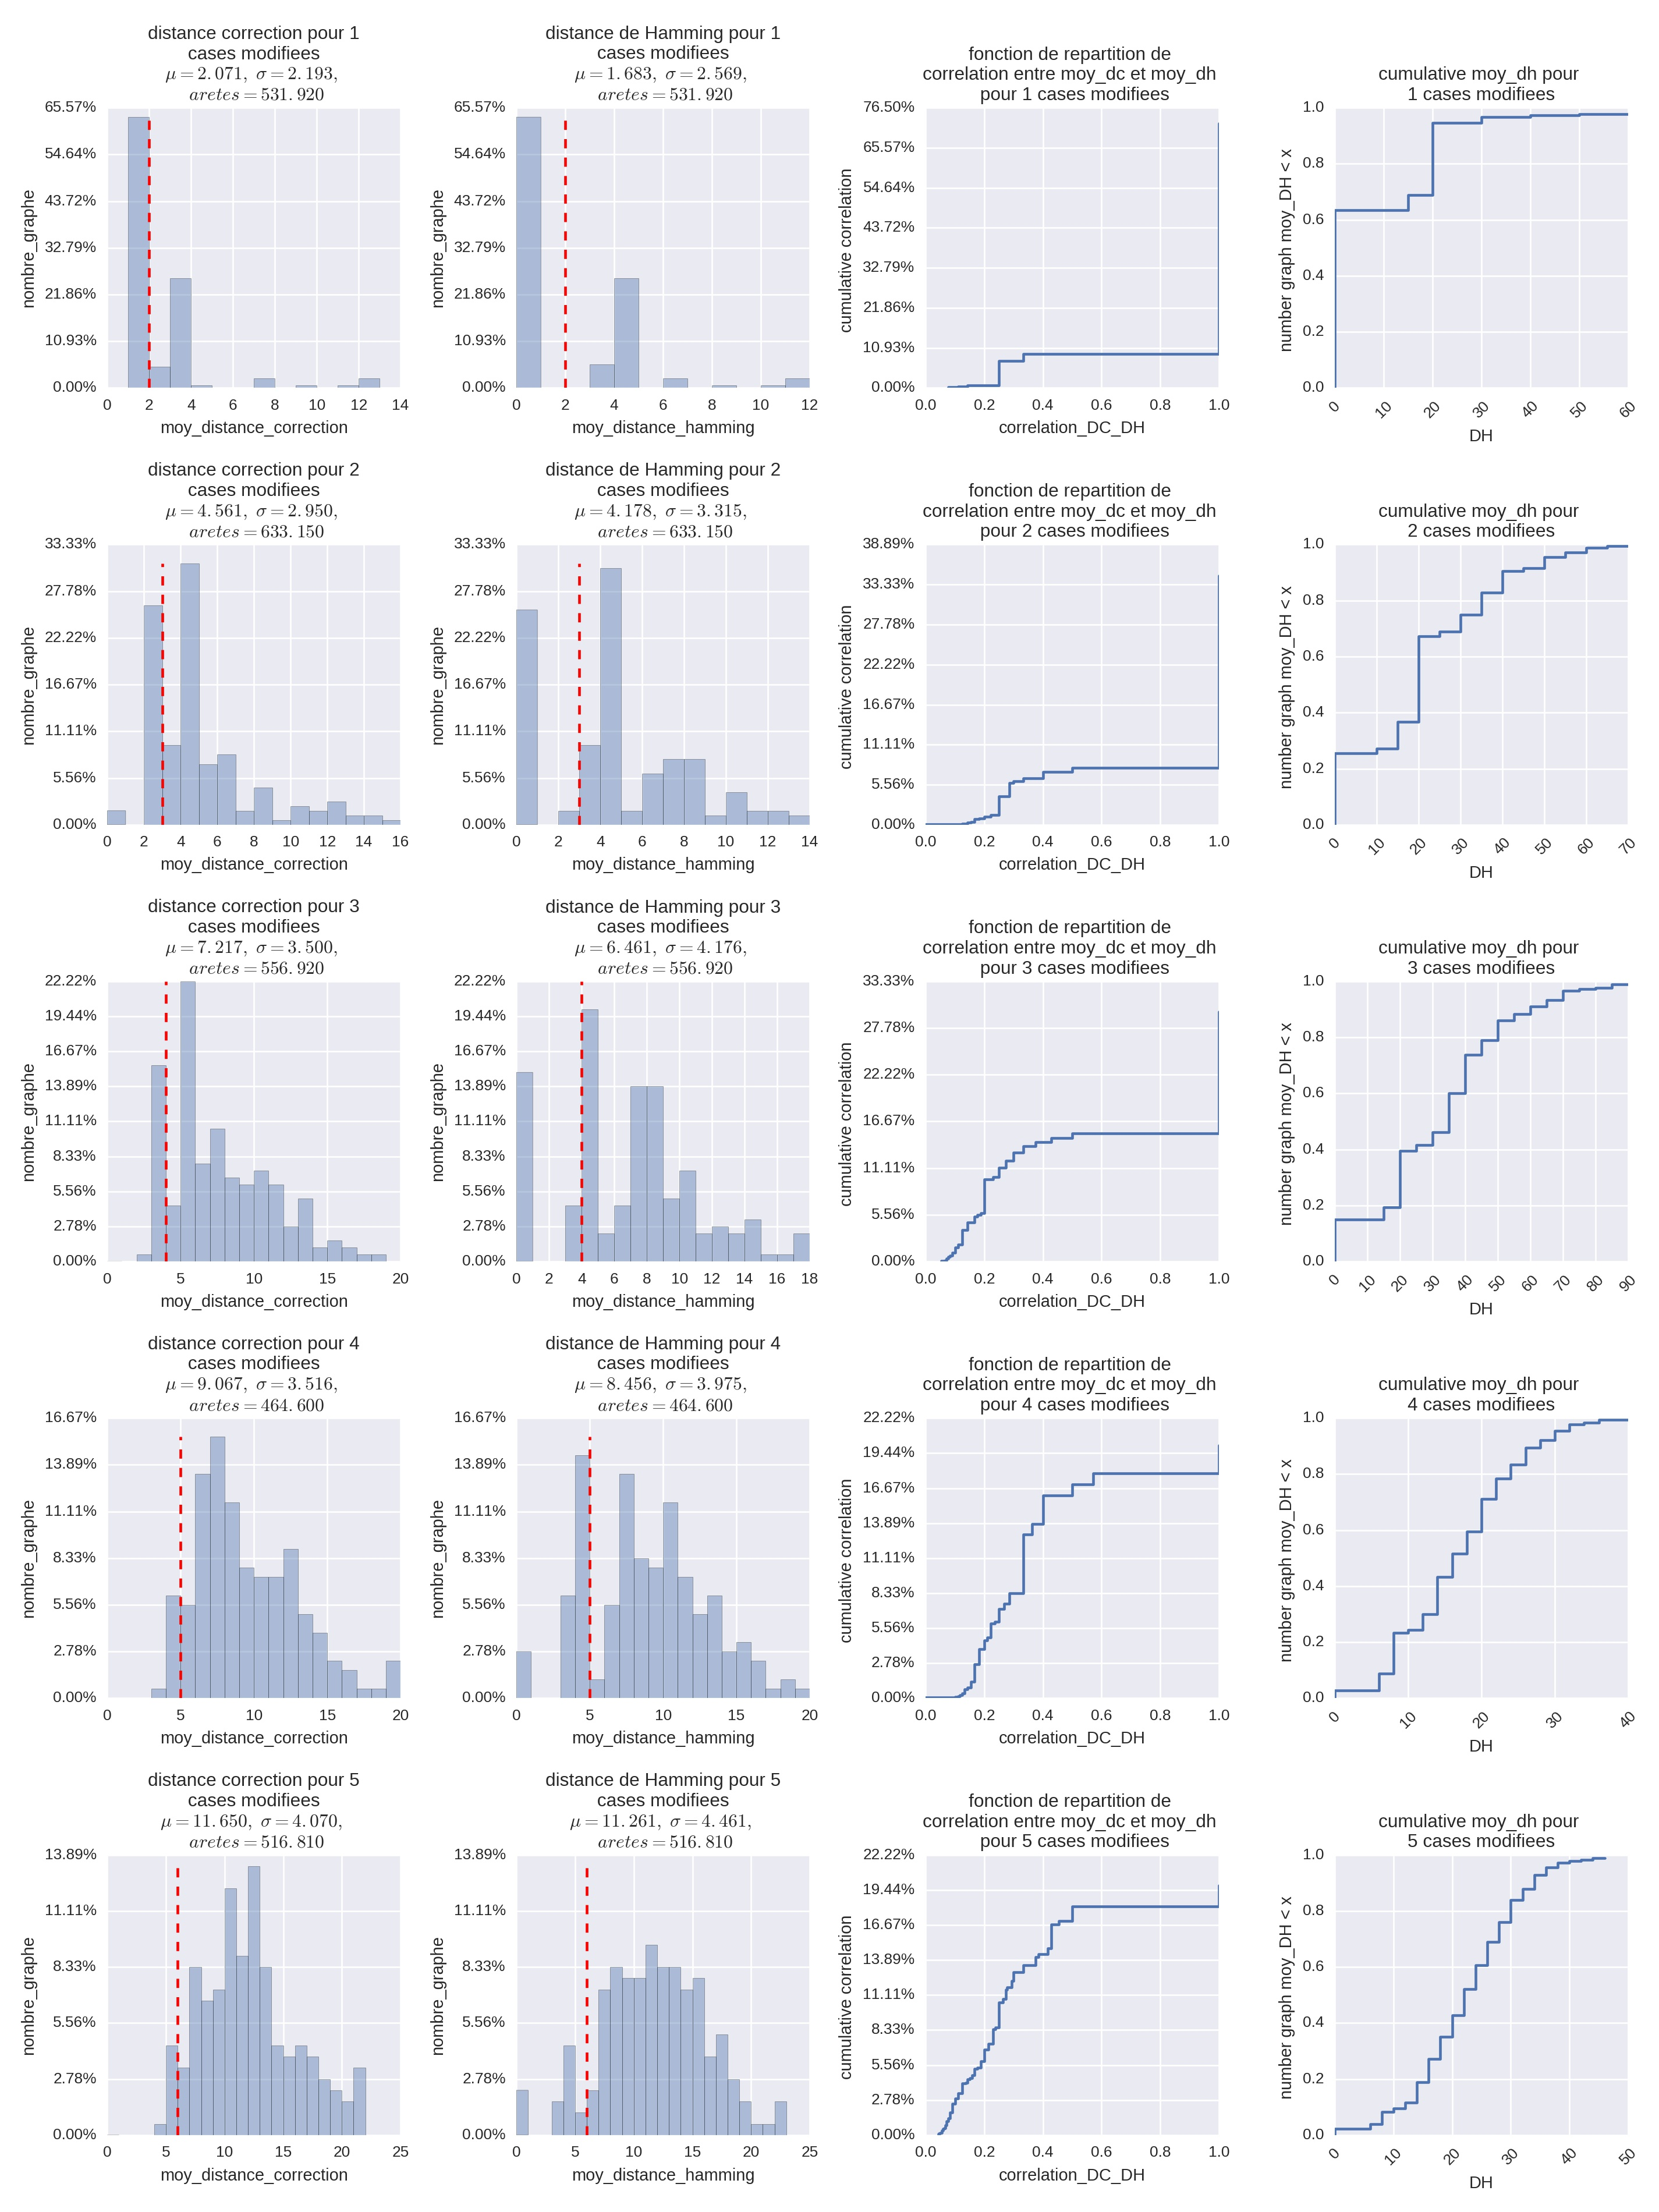
\includegraphics[width=550pt,height=580pt]{unitaire_aleatoire_sansRemise_distanceMoyenDLDH_k_1_2_3_4_5_p_05.jpeg}
\caption{ Approche de correction al\'eatoire sans remise \`a co\^ut unitaire pour $k =\{1,2,3,4,5\} $ cases modifi\'ees : La premi\`ere colonne repr\'esente la distribution des distances de correction $moy\_DC_{k,0.5}$. La seconde colonne est la distribution des distances de Hamming $moy\_DH_{k,0.5}$. La troisi\`eme colonne  est la fonction de repartition de la corr\'elation entre les distances de correction et de Hamming avec en abscisse la corr\'elation entre ces distances (correlation\_DC\_DH).  La quatri\`eme colonne est la fonction cumulative des distances de Hamming. La premi\`ere ligne est associ\'ee \`a $k=1$ case modifi\'ee, la seconde ligne \`a $k=2$ cases modifi\'ees, la troisi\`eme ligne \`a $5$ cases modifi\'ees et enfin la derni\`ere \`a $9$ cases modifi\'ees.}
\label{sansremise_unitaire_distanceMoyenDCDH_k_1_5_aleatoire_p_05} 
\end{figure}
\FloatBarrier

%{\large R\'esultats de la modification de $k \in \{6,7,8,9,\}$ cases avec $p=0.5$ }
\begin{figure}[htb!] 
\centering
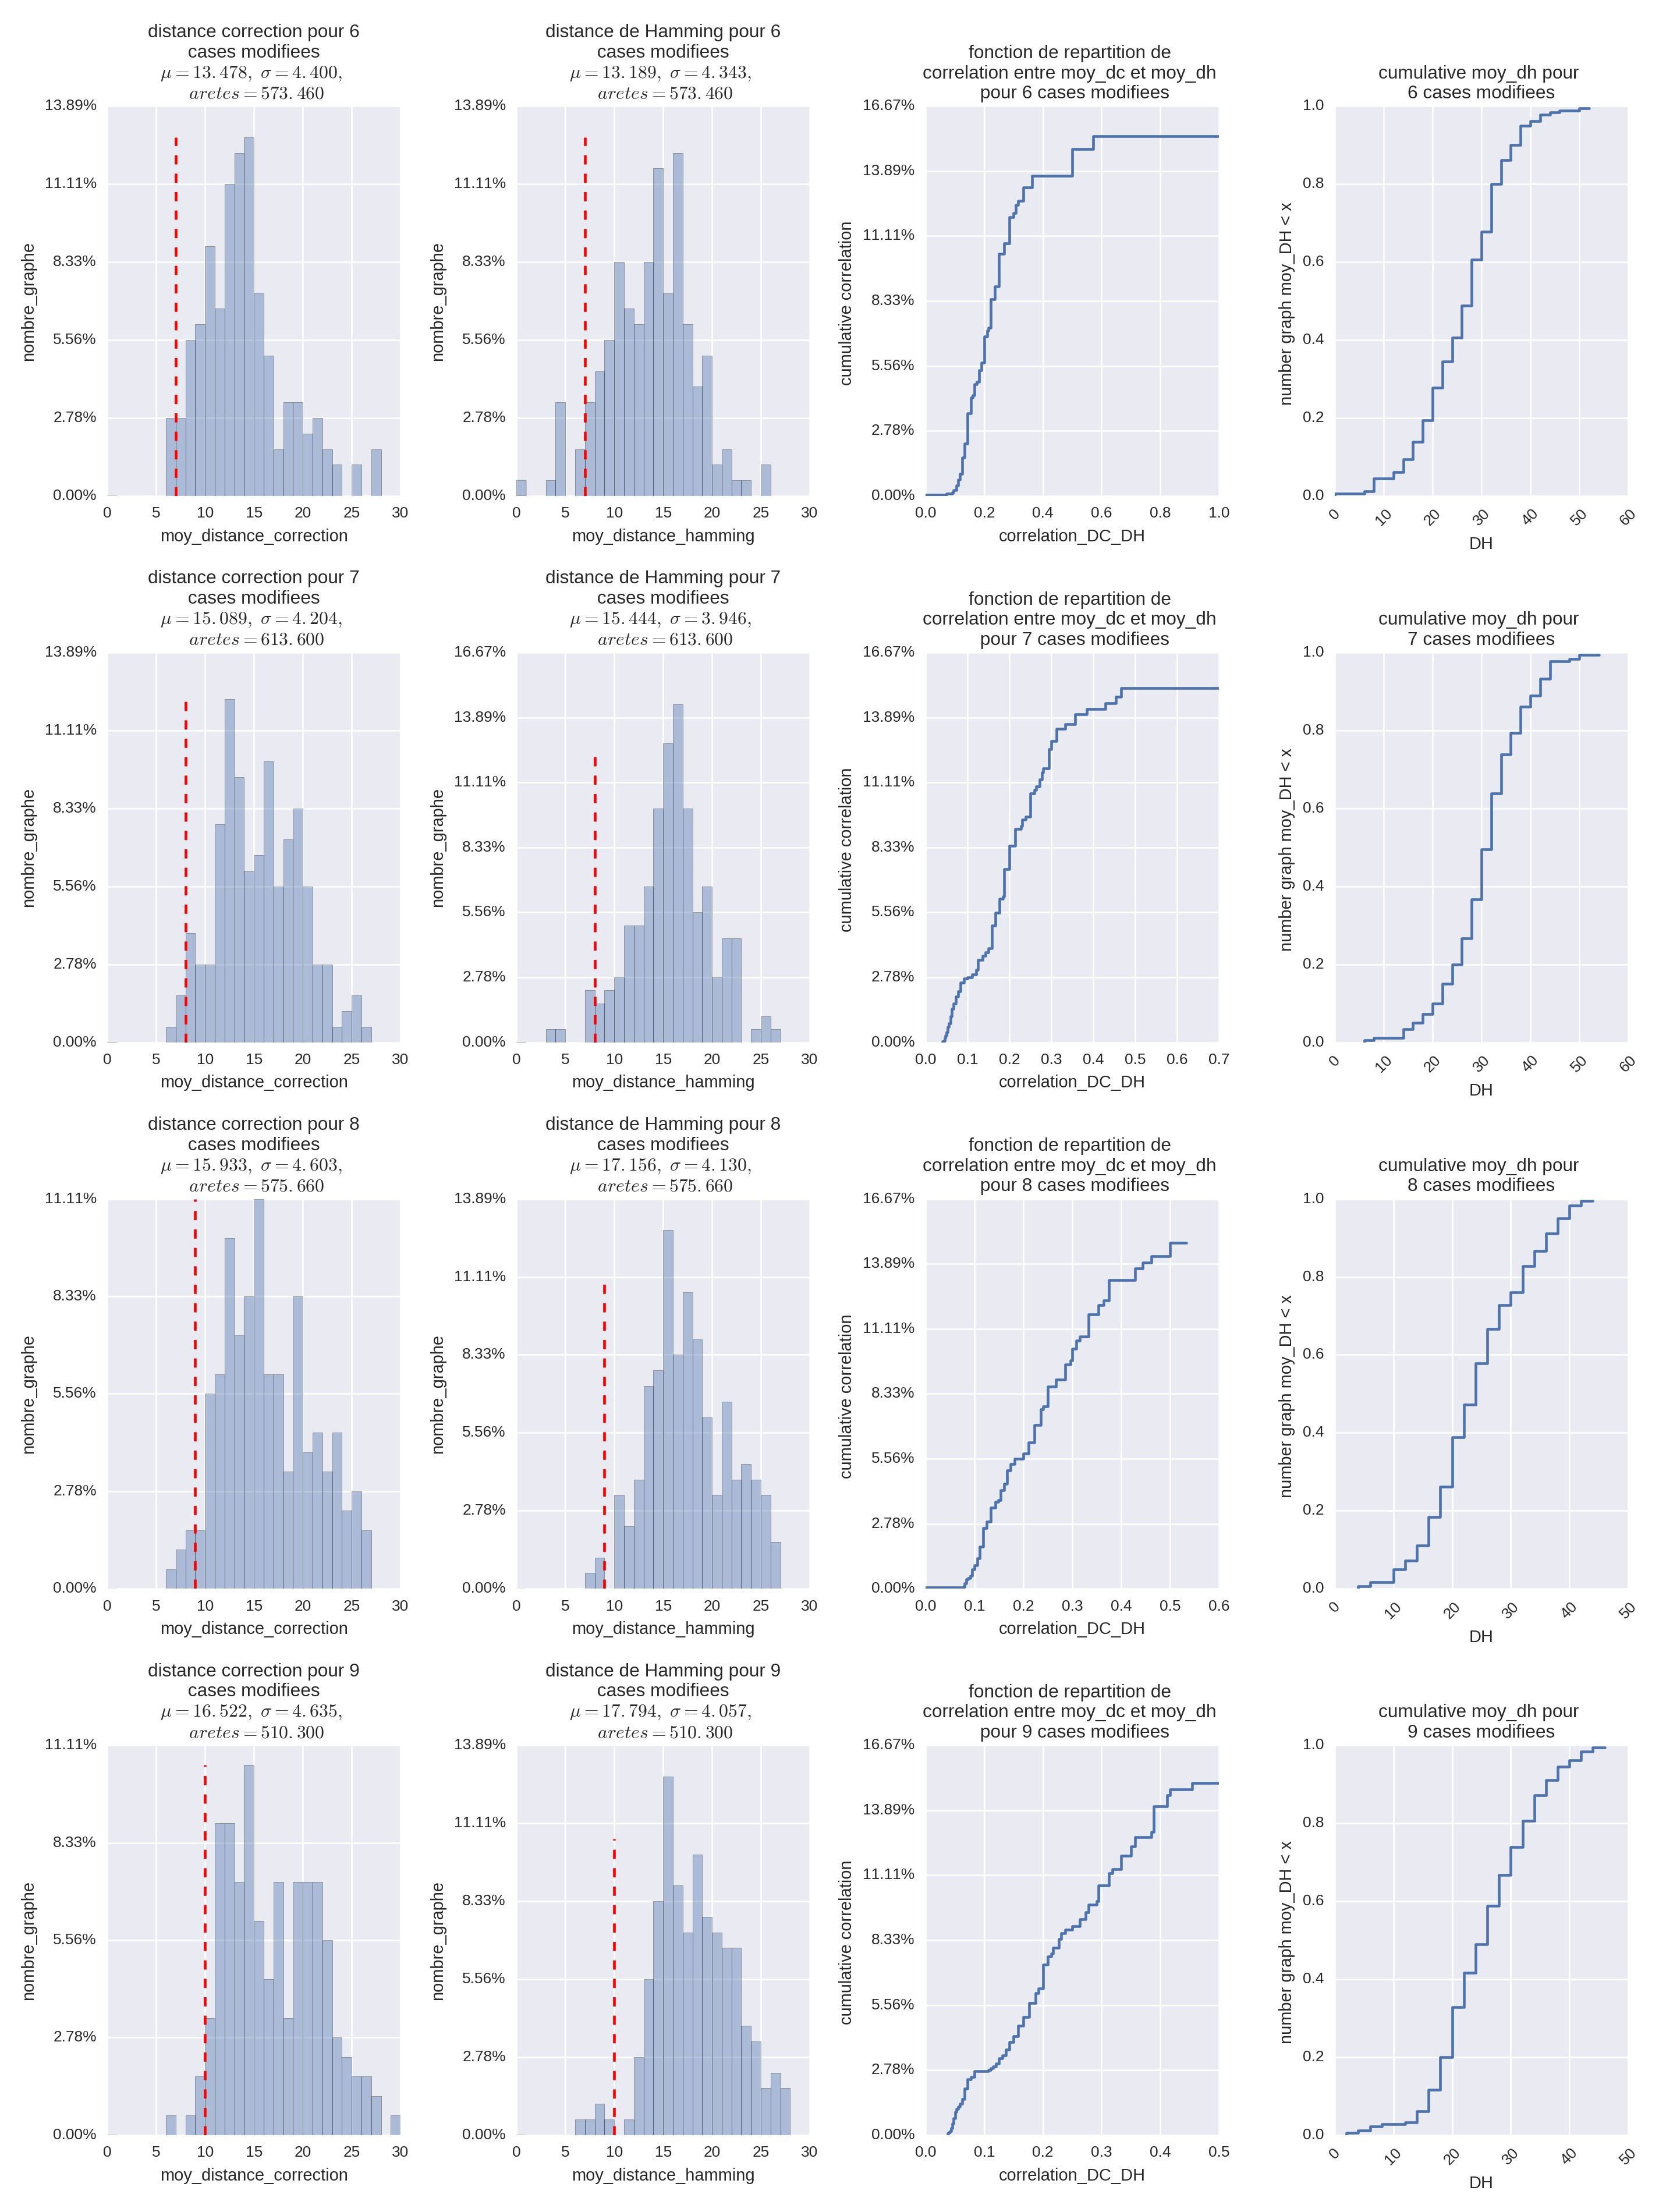
\includegraphics[width=550pt,height=580pt]{unitaire_aleatoire_sansRemise_distanceMoyenDLDH_k_6_7_8_9_p_05.jpeg}
\caption{ Approche de correction al\'eatoire sans remise \`a co\^ut unitaire pour $k =\{6,7,8,9\} $ cases modifi\'ees : La premi\`ere colonne repr\'esente la distribution des distances de correction $moy\_DC_{k,0.5}$. La seconde colonne est la distribution des distances de Hamming $moy\_DH_{k,0.5}$. La troisi\`eme colonne  est la fonction de repartition de la corr\'elation entre les distances de correction et de Hamming avec en abscisse la corr\'elation entre ces distances (correlation\_DL\_DH).  La quatri\`eme colonne est la fonction cumulative des distances de Hamming. La premi\`ere ligne est associ\'ee \`a $k=1$ case modifi\'ee, la seconde ligne \`a $k=2$ cases modifi\'ees, la troisi\`eme ligne \`a $5$ cases modifi\'ees et enfin la derni\`ere \`a $9$ cases modifi\'ees.}
\label{sansremise_unitaire_distanceMoyenDCDH_k_6_9_aleatoire_p_05} 
\end{figure}


\end{document}
